% Template for PLoS
%DIF LATEXDIFF DIFFERENCE FILE
%DIF DEL cbea.tex           Tue Nov 30 11:48:00 2021
%DIF ADD cbea_revised.tex   Wed Dec  1 19:09:41 2021
% Version 3.5 March 2018
%
% % % % % % % % % % % % % % % % % % % % % %
%
% -- IMPORTANT NOTE
%
% This template contains comments intended 
% to minimize problems and delays during our production 
% process. Please follow the template instructions
% whenever possible.
%
% % % % % % % % % % % % % % % % % % % % % % % 
%
% Once your paper is accepted for publication, 
% PLEASE REMOVE ALL TRACKED CHANGES in this file 
% and leave only the final text of your manuscript. 
% PLOS recommends the use of latexdiff to track changes during review, as this will help to maintain a clean tex file.
% Visit https://www.ctan.org/pkg/latexdiff?lang=en for info or contact us at latex@plos.org.
%
%
% There are no restrictions on package use within the LaTeX files except that 
% no packages listed in the template may be deleted.
%
% Please do not include colors or graphics in the text.
%
% The manuscript LaTeX source should be contained within a single file (do not use \input, \externaldocument, or similar commands).
%
% % % % % % % % % % % % % % % % % % % % % % %
%
% -- FIGURES AND TABLES
%
% Please include tables/figure captions directly after the paragraph where they are first cited in the text.
%
% DO NOT INCLUDE GRAPHICS IN YOUR MANUSCRIPT
% - Figures should be uploaded separately from your manuscript file. 
% - Figures generated using LaTeX should be extracted and removed from the PDF before submission. 
% - Figures containing multiple panels/subfigures must be combined into one image file before submission.
% For figure citations, please use "Fig" instead of "Figure".
% See http://journals.plos.org/plosone/s/figures for PLOS figure guidelines.
%
% Tables should be cell-based and may not contain:
% - spacing/line breaks within cells to alter layout or alignment
% - do not nest tabular environments (no tabular environments within tabular environments)
% - no graphics or colored text (cell background color/shading OK)
% See http://journals.plos.org/plosone/s/tables for table guidelines.
%
% For tables that exceed the width of the text column, use the adjustwidth environment as illustrated in the example table in text below.
%
% % % % % % % % % % % % % % % % % % % % % % % %
%
% -- EQUATIONS, MATH SYMBOLS, SUBSCRIPTS, AND SUPERSCRIPTS
%
% IMPORTANT
% Below are a few tips to help format your equations and other special characters according to our specifications. For more tips to help reduce the possibility of formatting errors during conversion, please see our LaTeX guidelines at http://journals.plos.org/plosone/s/latex
%
% For inline equations, please be sure to include all portions of an equation in the math environment.  For example, x$^2$ is incorrect; this should be formatted as $x^2$ (or $\mathrm{x}^2$ if the romanized font is desired).
%
% Do not include text that is not math in the math environment. For example, CO2 should be written as CO\textsubscript{2} instead of CO$_2$.
%
% Please add line breaks to long display equations when possible in order to fit size of the column. 
%
% For inline equations, please do not include punctuation (commas, etc) within the math environment unless this is part of the equation.
%
% When adding superscript or subscripts outside of brackets/braces, please group using {}.  For example, change "[U(D,E,\gamma)]^2" to "{[U(D,E,\gamma)]}^2". 
%
% Do not use \cal for caligraphic font.  Instead, use \mathcal{}
%
% % % % % % % % % % % % % % % % % % % % % % % % 
%
% Please contact latex@plos.org with any questions.
%
% % % % % % % % % % % % % % % % % % % % % % % %

\documentclass[10pt,letterpaper]{article}
\usepackage[top=0.85in,left=2.75in,footskip=0.75in]{geometry}

% amsmath and amssymb packages, useful for mathematical formulas and symbols
\usepackage{amsmath,amssymb}

% Use adjustwidth environment to exceed column width (see example table in text)
\usepackage{changepage}

% Use Unicode characters when possible
\usepackage[utf8x]{inputenc}

% textcomp package and marvosym package for additional characters
\usepackage{textcomp,marvosym}

% cite package, to clean up citations in the main text. Do not remove.
\usepackage{cite}

% Use nameref to cite supporting information files (see Supporting Information section for more info)
\usepackage{nameref,hyperref}

% line numbers
\usepackage[right]{lineno}

% ligatures disabled
\usepackage{microtype}
\DisableLigatures[f]{encoding = *, family = * }

% color can be used to apply background shading to table cells only
\usepackage[table]{xcolor}

% array package and thick rules for tables
\usepackage{array}

% create "+" rule type for thick vertical lines
\newcolumntype{+}{!{\vrule width 2pt}}

% create \thickcline for thick horizontal lines of variable length
\newlength\savedwidth
\newcommand\thickcline[1]{%
  \noalign{\global\savedwidth\arrayrulewidth\global\arrayrulewidth 2pt}%
  \cline{#1}%
  \noalign{\vskip\arrayrulewidth}%
  \noalign{\global\arrayrulewidth\savedwidth}%
}

% \thickhline command for thick horizontal lines that span the table
\newcommand\thickhline{\noalign{\global\savedwidth\arrayrulewidth\global\arrayrulewidth 2pt}%
\hline
\noalign{\global\arrayrulewidth\savedwidth}}


% Remove comment for double spacing
%\usepackage{setspace} 
%\doublespacing

% Text layout
\raggedright
\setlength{\parindent}{0.5cm}
\textwidth 5.25in 
\textheight 8.75in

% Bold the 'Figure #' in the caption and separate it from the title/caption with a period
% Captions will be left justified
\usepackage[aboveskip=1pt,labelfont=bf,labelsep=period,justification=raggedright,singlelinecheck=off]{caption}
\renewcommand{\figurename}{Fig}

% Use the PLoS provided BiBTeX style
\bibliographystyle{plos2015}

% Remove brackets from numbering in List of References
\makeatletter
\renewcommand{\@biblabel}[1]{\quad#1.}
\makeatother



% Header and Footer with logo
\usepackage{lastpage,fancyhdr,graphicx}
\usepackage{epstopdf}
%\pagestyle{myheadings}
\pagestyle{fancy}
\fancyhf{}
%\setlength{\headheight}{27.023pt}
%\lhead{\includegraphics[width=2.0in]{PLOS-submission.eps}}
\rfoot{\thepage/\pageref{LastPage}}
\renewcommand{\headrulewidth}{0pt}
\renewcommand{\footrule}{\hrule height 2pt \vspace{2mm}}
\fancyheadoffset[L]{2.25in}
\fancyfootoffset[L]{2.25in}
\lfoot{\today}

%% Include all macros below

\newcommand{\lorem}{{\bf LOREM}}
\newcommand{\ipsum}{{\bf IPSUM}}

%% END MACROS SECTION

% Adding packages 
\usepackage{bm}
\usepackage[parfill]{parskip}
\usepackage{float} %DIF > 
%DIF PREAMBLE EXTENSION ADDED BY LATEXDIFF
%DIF UNDERLINE PREAMBLE %DIF PREAMBLE
\RequirePackage[normalem]{ulem} %DIF PREAMBLE
\RequirePackage{color}\definecolor{RED}{rgb}{1,0,0}\definecolor{BLUE}{rgb}{0,0,1} %DIF PREAMBLE
\providecommand{\DIFaddtex}[1]{{\protect\color{blue}\uwave{#1}}} %DIF PREAMBLE
\providecommand{\DIFdeltex}[1]{{\protect\color{red}\sout{#1}}}                      %DIF PREAMBLE
%DIF SAFE PREAMBLE %DIF PREAMBLE
\providecommand{\DIFaddbegin}{} %DIF PREAMBLE
\providecommand{\DIFaddend}{} %DIF PREAMBLE
\providecommand{\DIFdelbegin}{} %DIF PREAMBLE
\providecommand{\DIFdelend}{} %DIF PREAMBLE
\providecommand{\DIFmodbegin}{} %DIF PREAMBLE
\providecommand{\DIFmodend}{} %DIF PREAMBLE
%DIF FLOATSAFE PREAMBLE %DIF PREAMBLE
\providecommand{\DIFaddFL}[1]{\DIFadd{#1}} %DIF PREAMBLE
\providecommand{\DIFdelFL}[1]{\DIFdel{#1}} %DIF PREAMBLE
\providecommand{\DIFaddbeginFL}{} %DIF PREAMBLE
\providecommand{\DIFaddendFL}{} %DIF PREAMBLE
\providecommand{\DIFdelbeginFL}{} %DIF PREAMBLE
\providecommand{\DIFdelendFL}{} %DIF PREAMBLE
%DIF HYPERREF PREAMBLE %DIF PREAMBLE
\providecommand{\DIFadd}[1]{\texorpdfstring{\DIFaddtex{#1}}{#1}} %DIF PREAMBLE
\providecommand{\DIFdel}[1]{\texorpdfstring{\DIFdeltex{#1}}{}} %DIF PREAMBLE
\newcommand{\DIFscaledelfig}{0.5}
%DIF HIGHLIGHTGRAPHICS PREAMBLE %DIF PREAMBLE
\RequirePackage{settobox} %DIF PREAMBLE
\RequirePackage{letltxmacro} %DIF PREAMBLE
\newsavebox{\DIFdelgraphicsbox} %DIF PREAMBLE
\newlength{\DIFdelgraphicswidth} %DIF PREAMBLE
\newlength{\DIFdelgraphicsheight} %DIF PREAMBLE
% store original definition of \includegraphics %DIF PREAMBLE
\LetLtxMacro{\DIFOincludegraphics}{\includegraphics} %DIF PREAMBLE
\newcommand{\DIFaddincludegraphics}[2][]{{\color{blue}\fbox{\DIFOincludegraphics[#1]{#2}}}} %DIF PREAMBLE
\newcommand{\DIFdelincludegraphics}[2][]{% %DIF PREAMBLE
\sbox{\DIFdelgraphicsbox}{\DIFOincludegraphics[#1]{#2}}% %DIF PREAMBLE
\settoboxwidth{\DIFdelgraphicswidth}{\DIFdelgraphicsbox} %DIF PREAMBLE
\settoboxtotalheight{\DIFdelgraphicsheight}{\DIFdelgraphicsbox} %DIF PREAMBLE
\scalebox{\DIFscaledelfig}{% %DIF PREAMBLE
\parbox[b]{\DIFdelgraphicswidth}{\usebox{\DIFdelgraphicsbox}\\[-\baselineskip] \rule{\DIFdelgraphicswidth}{0em}}\llap{\resizebox{\DIFdelgraphicswidth}{\DIFdelgraphicsheight}{% %DIF PREAMBLE
\setlength{\unitlength}{\DIFdelgraphicswidth}% %DIF PREAMBLE
\begin{picture}(1,1)% %DIF PREAMBLE
\thicklines\linethickness{2pt} %DIF PREAMBLE
{\color[rgb]{1,0,0}\put(0,0){\framebox(1,1){}}}% %DIF PREAMBLE
{\color[rgb]{1,0,0}\put(0,0){\line( 1,1){1}}}% %DIF PREAMBLE
{\color[rgb]{1,0,0}\put(0,1){\line(1,-1){1}}}% %DIF PREAMBLE
\end{picture}% %DIF PREAMBLE
}\hspace*{3pt}}} %DIF PREAMBLE
} %DIF PREAMBLE
\LetLtxMacro{\DIFOaddbegin}{\DIFaddbegin} %DIF PREAMBLE
\LetLtxMacro{\DIFOaddend}{\DIFaddend} %DIF PREAMBLE
\LetLtxMacro{\DIFOdelbegin}{\DIFdelbegin} %DIF PREAMBLE
\LetLtxMacro{\DIFOdelend}{\DIFdelend} %DIF PREAMBLE
\DeclareRobustCommand{\DIFaddbegin}{\DIFOaddbegin \let\includegraphics\DIFaddincludegraphics} %DIF PREAMBLE
\DeclareRobustCommand{\DIFaddend}{\DIFOaddend \let\includegraphics\DIFOincludegraphics} %DIF PREAMBLE
\DeclareRobustCommand{\DIFdelbegin}{\DIFOdelbegin \let\includegraphics\DIFdelincludegraphics} %DIF PREAMBLE
\DeclareRobustCommand{\DIFdelend}{\DIFOaddend \let\includegraphics\DIFOincludegraphics} %DIF PREAMBLE
\LetLtxMacro{\DIFOaddbeginFL}{\DIFaddbeginFL} %DIF PREAMBLE
\LetLtxMacro{\DIFOaddendFL}{\DIFaddendFL} %DIF PREAMBLE
\LetLtxMacro{\DIFOdelbeginFL}{\DIFdelbeginFL} %DIF PREAMBLE
\LetLtxMacro{\DIFOdelendFL}{\DIFdelendFL} %DIF PREAMBLE
\DeclareRobustCommand{\DIFaddbeginFL}{\DIFOaddbeginFL \let\includegraphics\DIFaddincludegraphics} %DIF PREAMBLE
\DeclareRobustCommand{\DIFaddendFL}{\DIFOaddendFL \let\includegraphics\DIFOincludegraphics} %DIF PREAMBLE
\DeclareRobustCommand{\DIFdelbeginFL}{\DIFOdelbeginFL \let\includegraphics\DIFdelincludegraphics} %DIF PREAMBLE
\DeclareRobustCommand{\DIFdelendFL}{\DIFOaddendFL \let\includegraphics\DIFOincludegraphics} %DIF PREAMBLE
%DIF LISTINGS PREAMBLE %DIF PREAMBLE
\RequirePackage{listings} %DIF PREAMBLE
\RequirePackage{color} %DIF PREAMBLE
\lstdefinelanguage{DIFcode}{ %DIF PREAMBLE
%DIF DIFCODE_UNDERLINE %DIF PREAMBLE
  moredelim=[il][\color{red}\sout]{\%DIF\ <\ }, %DIF PREAMBLE
  moredelim=[il][\color{blue}\uwave]{\%DIF\ >\ } %DIF PREAMBLE
} %DIF PREAMBLE
\lstdefinestyle{DIFverbatimstyle}{ %DIF PREAMBLE
	language=DIFcode, %DIF PREAMBLE
	basicstyle=\ttfamily, %DIF PREAMBLE
	columns=fullflexible, %DIF PREAMBLE
	keepspaces=true %DIF PREAMBLE
} %DIF PREAMBLE
\lstnewenvironment{DIFverbatim}{\lstset{style=DIFverbatimstyle}}{} %DIF PREAMBLE
\lstnewenvironment{DIFverbatim*}{\lstset{style=DIFverbatimstyle,showspaces=true}}{} %DIF PREAMBLE
%DIF END PREAMBLE EXTENSION ADDED BY LATEXDIFF

\begin{document}
\vspace*{0.2in}

% Title must be 250 characters or less.
\DIFdelbegin %DIFDELCMD < \begin{flushleft}
%DIFDELCMD < {\Large
%DIFDELCMD < \textbf\newline{cILR: Competitive isometric log-ratio for taxonomic enrichment analysis} % Please use "sentence case" for title and headings (capitalize only the first word in a title (or heading), the first word in a subtitle (or subheading), and any proper nouns).
%DIFDELCMD < }
%DIFDELCMD < %%%
\DIFdelend \DIFaddbegin \begin{flushleft}
{\Large
\textbf\newline{CBEA: Competitive balances for taxonomic enrichment analysis} % Please use "sentence case" for title and headings (capitalize only the first word in a title (or heading), the first word in a subtitle (or subheading), and any proper nouns).
}
\DIFaddend \newline
% Insert author names, affiliations and corresponding author email (do not include titles, positions, or degrees).
\\
Quang P. Nguyen\textsuperscript{1,2},
Anne G. Hoen\textsuperscript{1,2\ddag},
H. Robert Frost\textsuperscript{1*\ddag\dag},
\\
\bigskip
\textbf{1} Department of Biomedical Data Science, Geisel School of Medicine at Dartmouth College, Hanover, NH, USA
\\
\textbf{2} Department of Epidemiology, Geisel School of Medicine at Dartmouth College, Hanover, NH, USA
\\
\bigskip

% Insert additional author notes using the symbols described below. Insert symbol callouts after author names as necessary.
% 
% Remove or comment out the author notes below if they aren't used.
%
% Primary Equal Contribution Note
%\Yinyang These authors contributed equally to this work.

% Additional Equal Contribution Note
% Also use this double-dagger symbol for special authorship notes, such as senior authorship.
\ddag These authors jointly supervised this work.\\
\dag Corresponding author
% Current address notes
%\textcurrency Current Address: Dept/Program/Center, Institution Name, City, State, Country % change symbol to "\textcurrency a" if more than one current address note
% \textcurrency b Insert second current address 
% \textcurrency c Insert third current address

% Deceased author note
% \dag Deceased

% Group/Consortium Author Note
%\textpilcrow Membership list can be found in the Acknowledgments section.

% Use the asterisk to denote corresponding authorship and provide email address in note below.
* hildreth.r.frost@dartmouth.edu

\end{flushleft}
% Please keep the abstract below 300 words
\section*{Abstract}
Research in human associated microbiomes often involves the analysis of taxonomic count tables generated via high-throughput sequencing. It is difficult to apply statistical tools as the data is high-dimensional, sparse, and \DIFdelbegin \DIFdel{strictly }\DIFdelend compositional. An approachable way to alleviate high-dimensionality and sparsity is to aggregate variables into pre-defined sets. Set-based analysis is ubiquitous in the genomics literature, and has demonstrable impact in improving interpretability and power of downstream analysis. Unfortunately, there is a lack of sophisticated set-based analysis methods specific to microbiome taxonomic data, where current practice often employs abundance summation as a technique for aggregation. This approach prevents comparison across sets of different sizes, does not preserve inter-sample distances, and amplifies protocol bias. Here, we attempt to fill this gap with a new single sample taxon \DIFdelbegin \DIFdel{set enrichment method }\DIFdelend \DIFaddbegin \DIFadd{enrichment method with using a novel log-ratio formulation }\DIFaddend based on the \DIFdelbegin \DIFdel{isometric log ratio transformation and the }\DIFdelend competitive null hypothesis commonly used in the enrichment analysis literature. Our approach, titled competitive \DIFdelbegin \DIFdel{isometric log ratio (cILR}\DIFdelend \DIFaddbegin \DIFadd{balances for taxonomic enrichment analysis (CBEA}\DIFaddend ), generates sample-specific enrichment scores as the scaled log ratio of the subcomposition defined by taxa within a set and the subcomposition defined by its complement. We provide sample-level significance testing by estimating an empirical null distribution of our test statistic with valid p-values. Herein we demonstrate using both real data applications and simulations that \DIFdelbegin \DIFdel{cILR }\DIFdelend \DIFaddbegin \DIFadd{CBEA }\DIFaddend controls for type I error even under high sparsity and high inter-taxa correlation scenarios. Additionally, it provides informative scores that can be inputs to downstream \DIFdelbegin \DIFdel{differential abundance and }\DIFdelend \DIFaddbegin \DIFadd{analyses such as }\DIFaddend prediction tasks. 


% Please keep the Author Summary between 150 and 200 words
% Use first person. PLOS ONE authors please skip this step. 
% Author Summary not valid for PLOS ONE submissions.   
\section*{Author summary}
The study of human associated microbiomes relies on genomic surveys via high-throughput sequencing. However, microbiome taxonomic data is sparse and high dimensional which prevents the application of standard statistical techniques. One approach to address this problem is to perform analyses at the level of taxon sets. Set-based analysis has a long history in the genomics literature, with demonstrable impact in improving both power and interpretability. Unfortunately, there is not a lot of research in developing new set-based tools for microbiome taxonomic data specifically, given that compared to other 'omics data types microbiome taxonomic data is \DIFdelbegin \DIFdel{strictly }\DIFdelend compositional. We developed a new tool to generate taxon set enrichment scores at the sample level \DIFdelbegin \DIFdel{by combining the isometric }\DIFdelend \DIFaddbegin \DIFadd{through a novel }\DIFaddend log-ratio \DIFdelbegin \DIFdel{and }\DIFdelend \DIFaddbegin \DIFadd{formulation based on }\DIFaddend the competitive null hypothesis. Our scores can be used for statistical inference, and as inputs to other downstream analyses such as \DIFdelbegin \DIFdel{differential abundance and }\DIFdelend prediction models. We demonstrate the performance of our method against competing approaches across both real data analyses and simulation studies. 

\linenumbers

% Use "Eq" instead of "Equation" for equation citations.
\section*{Introduction}
The microbiome is the collection of microorganisms (bacteria, protozoa, archaea, fungi, and viruses) which co-exist with their host. Previous research has shown that changes in the composition of the human gut microbiome are associated with important health outcomes such as inflammatory bowel disease \cite{proctor2019}, type II diabetes \DIFdelbegin \DIFdel{\mbox{%DIFAUXCMD
\cite{sharma2019}}\hspace{0pt}%DIFAUXCMD
}\DIFdelend \DIFaddbegin \DIFadd{\mbox{%DIFAUXCMD
\cite{sharma2019a}}\hspace{0pt}%DIFAUXCMD
}\DIFaddend , and obesity \cite{aoun2020}. To understand the central role of the microbiome in human health, researchers have relied on high-throughput sequencing methods, either by targeting a specific representative gene (i.e. amplicon sequencing) or by profiling all the genomic content of the sample (i.e. whole-genome shotgun sequencing) \cite{cho2012}. Raw sequencing data is then processed through a variety of bioinformatic pipelines \cite{callahan2016, truong2015}, yielding various data products, one of which are taxonomic tables which can be used to study associations between members of the microbiome and an exposure or outcome of interest. 

However, there exists unique challenges in the analysis of these taxonomic count tables \DIFdelbegin \DIFdel{\mbox{%DIFAUXCMD
\cite{li2019,li2015}}\hspace{0pt}%DIFAUXCMD
. First, like other sequencing-based datasets, microbiome count data is often high dimensional, where the number of detected taxa far exceeds the number of samples usually present. For predictive tasks, microbiome-specific penalized regression approaches have been developed to address this issue \mbox{%DIFAUXCMD
\cite{shi2016}}\hspace{0pt}%DIFAUXCMD
, allowing for simultaneous model fitting and variable selection. For differential abundance tasks, researchers often utilize multiple hypothesis correction methods \mbox{%DIFAUXCMD
\cite{sankaran2014,benjamini1995} }\hspace{0pt}%DIFAUXCMD
or omnibus tests \mbox{%DIFAUXCMD
\cite{chen2018} }\hspace{0pt}%DIFAUXCMD
to address hypothesis testing burden. 
}%DIFDELCMD < 

%DIFDELCMD < %%%
\DIFdel{Second, the number of reads obtained is constrained by the sequencing instrument at an arbitrary limit, and is inconsistent across samples, resulting in a variable number of total read counts per sample. Many normalization methods \mbox{%DIFAUXCMD
\cite{weiss2017} }\hspace{0pt}%DIFAUXCMD
have been proposed to address these issues, including cross-applying methods from the gene expression literature \mbox{%DIFAUXCMD
\cite{mcmurdie2014}}\hspace{0pt}%DIFAUXCMD
. However, these methods rely on assumptions specific to the original bulk RNA-seq data sets such as the presence of housekeeping genes with consistent expression levels \mbox{%DIFAUXCMD
\cite{love2014}}\hspace{0pt}%DIFAUXCMD
, which might not be not true in the context of microbiome relative abundance data \mbox{%DIFAUXCMD
\cite{quinn2019,quinn2018b}}\hspace{0pt}%DIFAUXCMD
. As such, microbiome taxonomic data is strictly compositional \mbox{%DIFAUXCMD
\cite{gloor2017}}\hspace{0pt}%DIFAUXCMD
, which means that the abundance of any taxa can only be interpreted relative to another. Consequently, log-ratio transformations from the compositional data literature are often utilized \mbox{%DIFAUXCMD
\cite{aitchison1999}}\hspace{0pt}%DIFAUXCMD
. 
}%DIFDELCMD < 

%DIFDELCMD < %%%
\DIFdel{Third, the data are highly zero-inflated, where there is a high number of both structural zeros (truly missing due to biological reasons) and sampling zeroes (due to limits of detection of the sequencing experiment). Researchers often dealt with these issues by imputing zero cells with a pseudocount \mbox{%DIFAUXCMD
\cite{kurtz2015}}\hspace{0pt}%DIFAUXCMD
, or applying zero-inflated models \mbox{%DIFAUXCMD
\cite{chen2018, kaul2017}}\hspace{0pt}%DIFAUXCMD
. Newer methods developed recently have focused on understanding the different types of zeros in the data, providing more sophisticated heuristics around when pseudocounts can be utilized \mbox{%DIFAUXCMD
\cite{kaul2017a}}\hspace{0pt}%DIFAUXCMD
.   
}%DIFDELCMD < 

%DIFDELCMD < %%%
\DIFdelend \DIFaddbegin \DIFadd{\mbox{%DIFAUXCMD
\cite{li2019a,li2015}}\hspace{0pt}%DIFAUXCMD
. The data is sparse, high-dimensional, and likely compositional \mbox{%DIFAUXCMD
\cite{gloor2017, li2019a, li2015}}\hspace{0pt}%DIFAUXCMD
. }\DIFaddend Even though the \DIFdelbegin \DIFdel{aforementioned }\DIFdelend \DIFaddbegin \DIFadd{these }\DIFaddend problems are challenging, a very approachable \DIFdelbegin \DIFdel{method to address some of them is through }\DIFdelend \DIFaddbegin \DIFadd{solution is to to use }\DIFaddend set-based analysis \DIFaddbegin \DIFadd{methods}\DIFaddend , also termed gene set testing in the genomics literature \cite{khatri2012, goeman2007}. Aggregated \DIFdelbegin \DIFdel{sets are less sparsethan their constituent elements}\DIFdelend \DIFaddbegin \DIFadd{variables can be less sparse}\DIFaddend , and testing on a smaller number of \DIFdelbegin \DIFdel{variables reduces the multiple testing burden, thereby increasing }\DIFdelend \DIFaddbegin \DIFadd{features can reduce the multiple-testing burden. As such, gene set testing methods have been shown to increase }\DIFaddend power and reproducibility \DIFdelbegin \DIFdel{. Through }\DIFdelend \DIFaddbegin \DIFadd{of genomic analyses. Furthermore, through }\DIFaddend the usage of functionally informative sets defined apriori based on historical experiments (for example MSigDB \cite{subramanian2005}, and Gene Ontology \cite{ashburner2000}), gene set analyses also allows for more \DIFaddbegin \DIFadd{biologically }\DIFaddend informative interpretations. 
\DIFaddbegin 

\DIFaddend There exists a diverse set of \DIFdelbegin \DIFdel{available methods developed to perform such analyses. More traditional }\DIFdelend \DIFaddbegin \DIFadd{methods already developed in this field. Traditional }\DIFaddend set testing methods utilize the hypergeometric \DIFdelbegin \DIFdel{test }\DIFdelend \DIFaddbegin \DIFadd{distribution }\DIFaddend to test for the overrepresentation of \DIFdelbegin \DIFdel{significant p-values for a set of interest }\DIFdelend \DIFaddbegin \DIFadd{a gene set using a candidate list of genes screened based on a marginal model }\DIFaddend \cite{goeman2007}. Unfortunately, these approaches are sensitive to the differential expression test \DIFdelbegin \DIFdel{and their generated p-values. The most widely used gene-set analysis method, GSEA \mbox{%DIFAUXCMD
\cite{subramanian2005}}\hspace{0pt}%DIFAUXCMD
, instead uses a random-walk-like statistic through a ranking of genes based on a measure of association or effect size. Both of these methods generate enrichment scores and significance testing }\DIFdelend \DIFaddbegin \DIFadd{as well as the chosen threshold where genes can be part of the candidate list. Aggregate score methods, which are generally more preferred \mbox{%DIFAUXCMD
\cite{irizarry2009}}\hspace{0pt}%DIFAUXCMD
, instead assigns a score for each gene set based on gene-specific statistics such as z-scores or fold change. Of these approaches, methods such as GSEA \mbox{%DIFAUXCMD
\cite{subramanian2005} }\hspace{0pt}%DIFAUXCMD
performs a test for each gene set }\DIFaddend at the population level, \DIFdelbegin \DIFdel{incorporating information from }\DIFdelend \DIFaddbegin \DIFadd{summarizing information across }\DIFaddend all samples. Conversely, methods such as GSVA \cite{hanzelmann2013} and VAM \DIFdelbegin \DIFdel{\mbox{%DIFAUXCMD
\cite{frost2020a}}\hspace{0pt}%DIFAUXCMD
}\DIFdelend \DIFaddbegin \DIFadd{\mbox{%DIFAUXCMD
\cite{frost2020}}\hspace{0pt}%DIFAUXCMD
}\DIFaddend , generate enrichment scores at the sample level and are more akin to a transformation. \DIFdelbegin \DIFdel{This strategy }\DIFdelend \DIFaddbegin \DIFadd{In addition to being able to screen for enriched sets per sample, this strategy also }\DIFaddend allows for the flexible incorporation of different \DIFdelbegin \DIFdel{statistical techniques downstream }\DIFdelend \DIFaddbegin \DIFadd{downstream analyses}\DIFaddend , such as \DIFaddbegin \DIFadd{fitting }\DIFaddend prediction models, \DIFdelbegin \DIFdel{as well as for visualization purposes in ordination plots}\DIFdelend \DIFaddbegin \DIFadd{or performing dimension reduction}\DIFaddend .  

%DIF > First, like other sequencing-based datasets, microbiome count data is often high dimensional, where the number of detected taxa far exceeds the number of samples usually present. For predictive tasks, microbiome-specific penalized regression approaches have been developed to address this issue \cite{shi2016a}, allowing for simultaneous model fitting and variable selection. For differential abundance tasks, researchers often utilize multiple hypothesis correction methods \cite{sankaran2014,benjamini1995} or omnibus tests \cite{chen2018c} to address hypothesis testing burden. 
\DIFaddbegin 

%DIF > Second, the total number of reads varies across samples due to limitations of the sequencing instrument \cite{quinn2018}. 

%DIF > Third, the data are highly sparse, where there is a high number of both structural zeros (truly missing due to biological reasons) and sampling zeroes (due to limits of detection of the sequencing experiment). Researchers often dealt with these issues by imputing zero cells with a pseudocount \cite{kurtz2015a}, or applying zero-inflated models \cite{chen2018c, kaul2017}. Newer methods developed recently have focused on understanding the different types of zeros in the data, providing more sophisticated heuristics around when pseudocounts can be utilized \cite{kaul2017a}.   

\DIFaddend In microbiome research, even though no explicit enrichment analysis is performed, \DIFdelbegin \DIFdel{standard practice }\DIFdelend \DIFaddbegin \DIFadd{researchers }\DIFaddend often involves aggregating taxa to higher Linnean classification levels such as genus, family, or phylum\DIFdelbegin \DIFdel{by simple summation of abundances \mbox{%DIFAUXCMD
\cite{mclaren2019}}\hspace{0pt}%DIFAUXCMD
. Even though this allows for a reduction in the number of overall taxa (from thousands to only hundreds), there still exist three disadvantages: first, inter-sample distances are not preserved before and after aggregation \mbox{%DIFAUXCMD
\cite{egozcue2005}}\hspace{0pt}%DIFAUXCMD
, second, it doesn't allow for enrichment testing and comparison across sets of different sizes, and third, it increases bias when taxa within the set have different efficiencies in how they are measured through sequencing \mbox{%DIFAUXCMD
\cite{mclaren2019}}\hspace{0pt}%DIFAUXCMD
. As such, there is a need for microbiome researchers to adopt more robust sample-level set enrichment methods. Unfortunately, limited work has been }\DIFdelend \DIFaddbegin \DIFadd{. However, despite this interest, there is limited research }\DIFaddend done to extend existing \DIFdelbegin \DIFdel{methods to be more specific to }\DIFdelend \DIFaddbegin \DIFadd{set-based methods to }\DIFaddend microbiome relative abundance data. Some software suites, such as \emph{MicrobiomeAnalyst}, do offer tools to perform enrichment testing with curated taxon sets \cite{chong2020}. However, the approach used in \emph{MicrobiomeAnalyst} is a form of overrepresentation analysis at the population level and therefore similarly sensitive to the differential abundance approach used \DIFdelbegin \DIFdel{. 
}\DIFdelend \DIFaddbegin \DIFadd{and p-value threshold. One of the primary challenges for adapting gene set analysis to the microbiome context is the compositional nature of the data. Sequencing technologies constrain the total number of reads, and samples are expected to have the same number of reads instead of DNA content \mbox{%DIFAUXCMD
\cite{quinn2019, quinn2018}}\hspace{0pt}%DIFAUXCMD
. However, different samples still yield arbitrarily different total read counts \mbox{%DIFAUXCMD
\cite{morton2019, gloor2017}}\hspace{0pt}%DIFAUXCMD
, suggesting the use of normalization methods to allow for proper comparison of feature abundances across samples. However, microbiome data sets do not follow certain assumptions that enable the cross-application of methods from similar fields (such as RNA-seq) \mbox{%DIFAUXCMD
\cite{quinn2019, quinn2018}}\hspace{0pt}%DIFAUXCMD
. For example, DESeq2's }\emph{\DIFadd{estimateSizeFactors}} \DIFadd{\mbox{%DIFAUXCMD
\cite{love2014} }\hspace{0pt}%DIFAUXCMD
assumes that the majority of genes acts as housekeeping genes with constant expression levels across samples. As such, practitioners often rely on total sum normalization to transform count data into relative proportions that sum to one \mbox{%DIFAUXCMD
\cite{weiss2017}}\hspace{0pt}%DIFAUXCMD
. Empirical studies have supported this decision, showing increased performance of analysis tasks under this normalization schema \mbox{%DIFAUXCMD
\cite{mcknight2019}}\hspace{0pt}%DIFAUXCMD
. Since this approach imposes a sum constraint on the data, post normalization microbiome data sets are compositional \mbox{%DIFAUXCMD
\cite{gloor2017}}\hspace{0pt}%DIFAUXCMD
, which means that the abundance of any taxa can only be interpreted relative to another. Under this scenario, log-ratio based approaches from the compositional data analysis (CoDA) literature \mbox{%DIFAUXCMD
\cite{aitchison1999} }\hspace{0pt}%DIFAUXCMD
are motivated to address this issue. 
}\DIFaddend 

\DIFaddbegin \DIFadd{Standard practice for aggregating variables in microbiome research uses element-wise summations \mbox{%DIFAUXCMD
\cite{mclaren2019}}\hspace{0pt}%DIFAUXCMD
. Unfortunately, there are disadvantages to using this approach (referred to as amalgamations in the CoDA literature). First, inter-sample Aitchison distances computed on original parts are not preserved after amalgamation \mbox{%DIFAUXCMD
\cite{egozcue2005}}\hspace{0pt}%DIFAUXCMD
. This means that cluster analyses might show different results depending on the level of amalgamation and differs from the those computed from original variables. Second, amalgamations do not allow for comparison between sets of different sizes within the same experimental condition since larger sets will have larger means and variances. Third, considering that each taxa has specific measurement biases \mbox{%DIFAUXCMD
\cite{mclaren2019}}\hspace{0pt}%DIFAUXCMD
, an amalgamation based approach would make the bias of the amalgamated variable dependent on the relative abundance of the its constituents. In other words, if taxon $1$ has abundance $A_1$ and bias $B_1$, while taxon $2$ has abundance $A_2$ and bias $B_2$, then the bias of the aggregate variable (for example, a genera) is $(A_1B_1 + A_2B_2)/(A_1 + A_2)$ (see Appendix 1. from McLaren et al. \mbox{%DIFAUXCMD
\cite{mclaren2019}}\hspace{0pt}%DIFAUXCMD
). This means that bias invariant approaches (such as analyses of ratios) would no longer be invariant when applied to amalgamated variables as bias now varies across samples. The alternative would be to multiply the proportions rather than to sum them \mbox{%DIFAUXCMD
\cite{egozcue2005}}\hspace{0pt}%DIFAUXCMD
. 
}

\DIFaddend Here, we present a \DIFdelbegin \DIFdel{novel method that }\DIFdelend \DIFaddbegin \DIFadd{taxon-set testing method for microbiome relative abundance data that addresses the aforementioned issues. Our approach }\DIFaddend generates enrichment scores at the sample level similar to GSVA \cite{hanzelmann2013} and VAM \DIFdelbegin \DIFdel{\mbox{%DIFAUXCMD
\cite{frost2020a}}\hspace{0pt}%DIFAUXCMD
}\DIFdelend \DIFaddbegin \DIFadd{\mbox{%DIFAUXCMD
\cite{frost2020}}\hspace{0pt}%DIFAUXCMD
}\DIFaddend . We leverage the concept of the $Q_1$ competitive hypothesis presented in Tian et al. \cite{tian2005} \DIFdelbegin \DIFdel{, which tests the null that the value of variables within a specific set is equal to the value of measured variables not in the set . The competitive null hypothesis is particularly useful in compositional data analysis, as it naturally assesses enrichment as a ratio between two sets of variables. We incorporated this insight with the isometric log-ratio transformation \mbox{%DIFAUXCMD
\cite{egozcue2003}}\hspace{0pt}%DIFAUXCMD
, which allows for a multiplicative aggregation method that addresses the downsides of the naive summation-based method presented above \mbox{%DIFAUXCMD
\cite{mclaren2019, silverman2017}}\hspace{0pt}%DIFAUXCMD
. The resulting method, titled competitive isometric log-ratio (cILR), is therefore unsupervised and can generate sample-specific enrichment scores with a }\DIFdelend \DIFaddbegin \DIFadd{to formulate the enrichment of a set as the compositional balance \mbox{%DIFAUXCMD
\cite{rivera-pinto} }\hspace{0pt}%DIFAUXCMD
of taxa within the set and remainder taxa using multiplication as the method of aggregating proportions \mbox{%DIFAUXCMD
\cite{egozcue2005}}\hspace{0pt}%DIFAUXCMD
. This }\DIFaddend well-defined null hypothesis \DIFdelbegin \DIFdel{that allows for significance testing . These scores can then act as inputs to differential abundance and predictive modeling tasks downstream}\DIFdelend \DIFaddbegin \DIFadd{allows us to perform significance testing with interpretable results through estimating the empirical distribution of our statistic under the null that can also account for variance inflation due to inter-taxa correlation \mbox{%DIFAUXCMD
\cite{wu2012}}\hspace{0pt}%DIFAUXCMD
}\DIFaddend . 

In the following sections, we \DIFdelbegin \DIFdel{provide the formulation of cILR and discuss some }\DIFdelend \DIFaddbegin \DIFadd{present our approach titled competitive balances for taxonomic erichment analysis (CBEA). First, we presented the step-by-step formulation of CBEA and discuss its }\DIFaddend statistical properties. \DIFdelbegin \DIFdel{We illustrate significance testing at the sample level using cILR and evaluate type I error and power under different simulation scenarios and real data applications. We assess the informativeness of cILR generated scores, and evaluate how it performs as part of downstream analyses, specifically predictive models and differential abundance analysis. We compare the performance of cILR in these respective tasks againststandard microbiome taxonomic data analysis practices, }\DIFdelend \DIFaddbegin \DIFadd{Second, we detailed our evaluation strategy using both real data and parametric simulations, and the methods we're comparing against. Third, we presented results on enrichment testing using CBEA for single samples }\DIFaddend as well as \DIFdelbegin \DIFdel{the existing GSVA \mbox{%DIFAUXCMD
\cite{hanzelmann2013} }\hspace{0pt}%DIFAUXCMD
and ssGSEA \mbox{%DIFAUXCMD
\cite{barbie2009}}\hspace{0pt}%DIFAUXCMD
, which are single sample methods. }\DIFdelend \DIFaddbegin \DIFadd{at the population level. Fourth, we showed the performance of CBEA in downstream disease prediction. Finally, we discussed our results and the limitations of our method. }\DIFaddend An R package implementation of \DIFdelbegin \DIFdel{this approach }\DIFdelend \DIFaddbegin \DIFadd{CBEA }\DIFaddend can be found on \DIFdelbegin \DIFdel{Github (}\DIFdelend \DIFaddbegin \DIFadd{GitHub (}\DIFaddend \href{www.github.com/qpmnguyen/teaR}{qpmnguyen/\DIFdelbegin \DIFdel{teaR}\DIFdelend \DIFaddbegin \DIFadd{CBEA}\DIFaddend }).

\section*{Materials and Methods} \label{methods}
\subsection*{Competitive \DIFdelbegin \DIFdel{Isometric Log-ratio }\DIFdelend \DIFaddbegin \DIFadd{balances for taxonomic enrichment analysis }\DIFaddend (\DIFdelbegin \DIFdel{cILR}\DIFdelend \DIFaddbegin \DIFadd{CBEA}\DIFaddend )}
The \DIFdelbegin \DIFdel{cILR }\DIFdelend \DIFaddbegin \DIFadd{CBEA }\DIFaddend method generates sample-specific enrichment scores for microbial sets using the isometric log-ratio transformation \cite{egozcue2003}. Details on the computational implementation of \DIFdelbegin \DIFdel{cILR }\DIFdelend \DIFaddbegin \DIFadd{CBEA }\DIFaddend can be found in the supplemental materials. The \DIFdelbegin \DIFdel{cILR }\DIFdelend \DIFaddbegin \DIFadd{CBEA }\DIFaddend method takes two inputs:  
\begin{itemize}
    \item $\mathbf{X}$: $n$ by $p$ matrix of positive counts for $p$ taxa and $n$ samples measured through either targeted sequencing (such as of the 16S rRNA gene) or whole genome shotgun sequencing. Usually $\mathbf{X}$ is generated from standard taxonomic profiling pipelines such as DADA2 \cite{callahan2016} for 16S rRNA sequencing, or MetaPhlAn2 \cite{truong2015} for whole genome shotgun sequencing. 
    \item $\mathbf{A}$: $p$ by $m$ indicator matrix annotating the membership of each taxon $p$ to $m$ sets of interest. These sets can be Linnean taxonomic classifications annotated using databases such as SILVA \cite{quast2013}, or those based on more functionally driven categories such as tropism or ecosystem roles ($A_{i,j} = 1$ indicates that microbe $i$ belongs to set $j$). 
\end{itemize}
The \DIFdelbegin \DIFdel{cILR }\DIFdelend \DIFaddbegin \DIFadd{CBEA }\DIFaddend method generates one output:  
\begin{itemize} 
    \item $\mathbf{E}$: $n$ by $m$ matrix indicating the enrichment score of $m$ pre-defined sets identified in $\mathbf{A}$ across $n$ samples. 
\end{itemize}
The procedure is as follows:  
\begin{enumerate}
    \item \textbf{Compute the \DIFdelbegin \DIFdel{cILR }\DIFdelend \DIFaddbegin \DIFadd{CBEA }\DIFaddend statistic}: Let $\mathbf{M}$ be a $n$ by $m$ matrix of \DIFdelbegin \DIFdel{cILR }\DIFdelend \DIFaddbegin \DIFadd{CBEA }\DIFaddend scores. Let $\mathbf{M}_{i,k}$ be \DIFdelbegin \DIFdel{cILR }\DIFdelend \DIFaddbegin \DIFadd{CBEA }\DIFaddend scores for set $k$ of sample $i$:   
    \begin{equation}\label{main_eq}
        \mathbf{M}_{i,k} = \sqrt{\frac{\sum_k A_{ik}(p - \sum_k A_{ik})}{p}} \ln \left( \frac{g(\mathbf{X}_{i,j}|\mathbf{A}_{j,k} = 1)}{g(\mathbf{X}_{i,j}|\mathbf{A}_{j,k} \neq 1))} \right)
    \end{equation}
    where $g(.)$ is the geometric mean. This represents the ratio of the geometric mean of the relative abundance of taxa assigned to set $k$ and remainder taxa. 
    \item \textbf{Estimate the empirical null distribution} Enrichment scores represent the test statistic for the $Q_1$ null hypothesis $H_o$ that relative abundances in $\mathbf{X}$ of members of set $k$ are not enriched compared to those not in set $k$. Since the distribution of \DIFdelbegin \DIFdel{cILR }\DIFdelend \DIFaddbegin \DIFadd{CBEA }\DIFaddend under the null vary depending on data characteristics (Fig~\ref{fig:1}), an empirical null distribution will be estimated from data.
    \begin{itemize}
        \item \textbf{Compute the \DIFdelbegin \DIFdel{cILR }\DIFdelend \DIFaddbegin \DIFadd{CBEA }\DIFaddend statistic on permuted and un-permuted $\mathbf{X}$}.  Let $\mathbf{X}_{perm}$ be the column permuted relative abundance matrix, and $\mathbf{M}_{perm}$ be the corresponding \DIFdelbegin \DIFdel{cILR }\DIFdelend \DIFaddbegin \DIFadd{CBEA }\DIFaddend scores generated from $\mathbf{X}_{perm}$. Similarly, we have $\mathbf{M}_{unperm}$ be \DIFdelbegin \DIFdel{cILR }\DIFdelend \DIFaddbegin \DIFadd{CBEA }\DIFaddend scores generated from $\mathbf{X}$.
        \item \textbf{Estimate correlation-adjusted empirical distribution for each set}. For each set, a fit a parametric distribution to both $\mathbf{M}_{perm}$ and $\mathbf{M}_{unperm}$. The location measure estimated from $\mathbf{M}_{perm}$ and the spread measure estimated from $\mathbf{M}_{unperm}$ will be combined as the correlation-adjusted empirical null distribution $\mathbf{P}_{emp}$ for each set. Two available options are the normal distribution and the mixture normal distribution. For the normal distribution, parameters were estimated using the method of maximum likelihood implemented in the \emph{fitdistr} package \cite{delignette-muller2015}. For the mixture normal distribution, parameters were estimated using an expectation-maximization algorithm implemented in the \emph{mixtools} package \cite{benaglia2009}. 
    \end{itemize}
    \item \textbf{Calculate finalized \DIFdelbegin \DIFdel{cILR }\DIFdelend \DIFaddbegin \DIFadd{CBEA }\DIFaddend scores with respect to the empirical null}. Enrichment scores $\mathbf{E}_{i,k}$ are calculated as the cumulative distribution function (CDF) values or z-scores with respect to $\mathbf{P}_{emp}$ distribution. P-values can be calculated by subtracting $\mathbf{E}$ from 1. 
\end{enumerate}

\subsection*{Properties of \DIFdelbegin \DIFdel{cILR}\DIFdelend \DIFaddbegin \DIFadd{CBEA}\DIFaddend }
\subsubsection*{\DIFdelbegin \DIFdel{cILR }\DIFdelend \DIFaddbegin \DIFadd{CBEA }\DIFaddend and \DIFdelbegin \DIFdel{the Isometric Log Ratio Transformation}\DIFdelend \DIFaddbegin \DIFadd{balances of groups of parts}\DIFaddend }
The \DIFdelbegin \DIFdel{cILR }\DIFdelend \DIFaddbegin \DIFadd{CBEA }\DIFaddend statistic is a special instance of the isometric log-ratio transformation (ILR) \cite{egozcue2003}. The standard ILR is a transformation method to address the negative correlation bias inherent in compositional data by providing an isometry between the $D$-dimensional simplex $\mathbb{S}^D$ and coordinates in the $D-1$ real space $\mathbb{R}^{D-1}$ \cite{egozcue2003,washburne2017}. This is accomplished by projecting the composition onto a chosen orthonormal basis in $\mathbb{R}$, which can be defined by a sequential binary partition (SBP) of the variables (e.g. a rooted phylogenetic tree). The ILR transformed variables are the coordinates of nodes within an SBP tree of the variables. Without loss of generalizability, in a given SBP with node $i$ splitting variables between sets $R$ and $S$, we have the ILR coordinate $x^{*}_{i}$ as: 
\begin{equation}\label{ilr_standard}
    x^{*}_i = \sqrt{\frac{rs}{r+s}} \log\left(\frac{g(X_{j|j \in R})}{g(X_{j|j \in S})}\right)
\end{equation}
where $r$ and $s$ are the cardinalities of sets $R$ and $S$ respectively, $g(z)$ is the geometric mean, and $X_{j}$ are values of the original predictors with indexes defined by membership in $R$ and $S$. The ILR confer many important benefits. First, ILR coordinates exist in real space, whereby common statistical methods can be used. Second, ILR aggregated variables preserve inter-sample distances before and after aggregation \cite{egozcue2005}. Third, ILR variables are not constrained to sum to 0 as that of the centered log-ratio transformation, resulting in a covariance matrix that is not singular \cite{egozcue2003}. 

The usage of the ILR statistic is not uncommon in the microbiome literature. They are usually termed ``compositional balances", and have been leveraged in many recent approaches in variable transformation \cite{washburne2017,silverman2017,morton2017}. The \DIFdelbegin \DIFdel{cILR }\DIFdelend \DIFaddbegin \DIFadd{CBEA }\DIFaddend formulation in Eq~\eqref{main_eq} is a special case of Eq~\eqref{ilr_standard} defined on a node that splits the taxa into two disjoint sets, one representing the set of interest, the other representing the remaining taxa. As such, the \DIFdelbegin \DIFdel{cILR }\DIFdelend \DIFaddbegin \DIFadd{CBEA }\DIFaddend transformation inherits the properties of the ILR as a log-ratio method applicable to compositional data sets. However, unlike the ILR and its variants \cite{silverman2017, morton2017, washburne2017}, the axes defined by each \DIFdelbegin \DIFdel{cILR }\DIFdelend \DIFaddbegin \DIFadd{CBEA }\DIFaddend set are not orthogonal (since the balances are mutually exclusive between sets and do not belong in the same SBP). Hence, a correlation can exist between \DIFdelbegin \DIFdel{cILR }\DIFdelend \DIFaddbegin \DIFadd{CBEA }\DIFaddend aggregated variables.  

\subsubsection*{\DIFdelbegin \DIFdel{Statistical Properties of cILR}\DIFdelend \DIFaddbegin \DIFadd{Estimating the null distribution}\DIFaddend }
We can perform significance testing on the \DIFdelbegin \DIFdel{cILR }\DIFdelend \DIFaddbegin \DIFadd{CBEA }\DIFaddend statistic which corresponds to the null hypothesis that the center of the subcomposition defined by the set is equal to the center of the subcomposition defined by the complement of the set. This is equivalent to the $Q_1$ competitive null hypothesis in the gene set testing literature \cite{tian2005} where the enrichment of a gene set is defined with respect to genes outside the set. 

We can apply prior usage of the ILR statistic in hypothesis testing to \DIFdelbegin \DIFdel{cILR }\DIFdelend \DIFaddbegin \DIFadd{CBEA }\DIFaddend by assuming that the null distribution of \DIFdelbegin \DIFdel{cILR }\DIFdelend \DIFaddbegin \DIFadd{CBEA }\DIFaddend follows a standard normal distribution \cite{egozcue2005}. However, when applying \DIFdelbegin \DIFdel{cILR }\DIFdelend \DIFaddbegin \DIFadd{CBEA }\DIFaddend for hypothesis testing at the sample level, it is expected that the researcher would be testing a large number of hypotheses. Under the assumption that the number of truly significant hypotheses is low, Efron \cite{efron2004} showed that estimating the null distribution of the test statistic (termed the empirical null distribution) is much more preferable than using the theoretical null due to unobserved confounding effects inherently part of observational studies. As such, to perform significance testing using \DIFdelbegin \DIFdel{cILR}\DIFdelend \DIFaddbegin \DIFadd{CBEA}\DIFaddend , we also estimated the null distribution from observed raw \DIFdelbegin \DIFdel{cILR }\DIFdelend \DIFaddbegin \DIFadd{CBEA }\DIFaddend variables. 

This assumption is also supported by preliminary simulation studies (detailed below). In panel A of Fig~\ref{fig:1}, we simulated microbiome taxonomic count data under the global null across different data features and compute raw \DIFdelbegin \DIFdel{cILR }\DIFdelend \DIFaddbegin \DIFadd{CBEA }\DIFaddend scores and compute kurtosis and skewness. It can be seen that the characteristics of the null change depending on sparsity and inter-taxa correlation. Sparsity seems to drive the distribution to be more positively skewed while inter-taxa correlation encourages platykurtic (negative kurtosis). The effect is most dramatic under both high inter-taxa correlation and sparsity. This heterogeneity further supports the decision to estimate an empirical null distribution, similar to Efron \cite{efron2004}. 

\begin{figure} [!h]
    \centering
    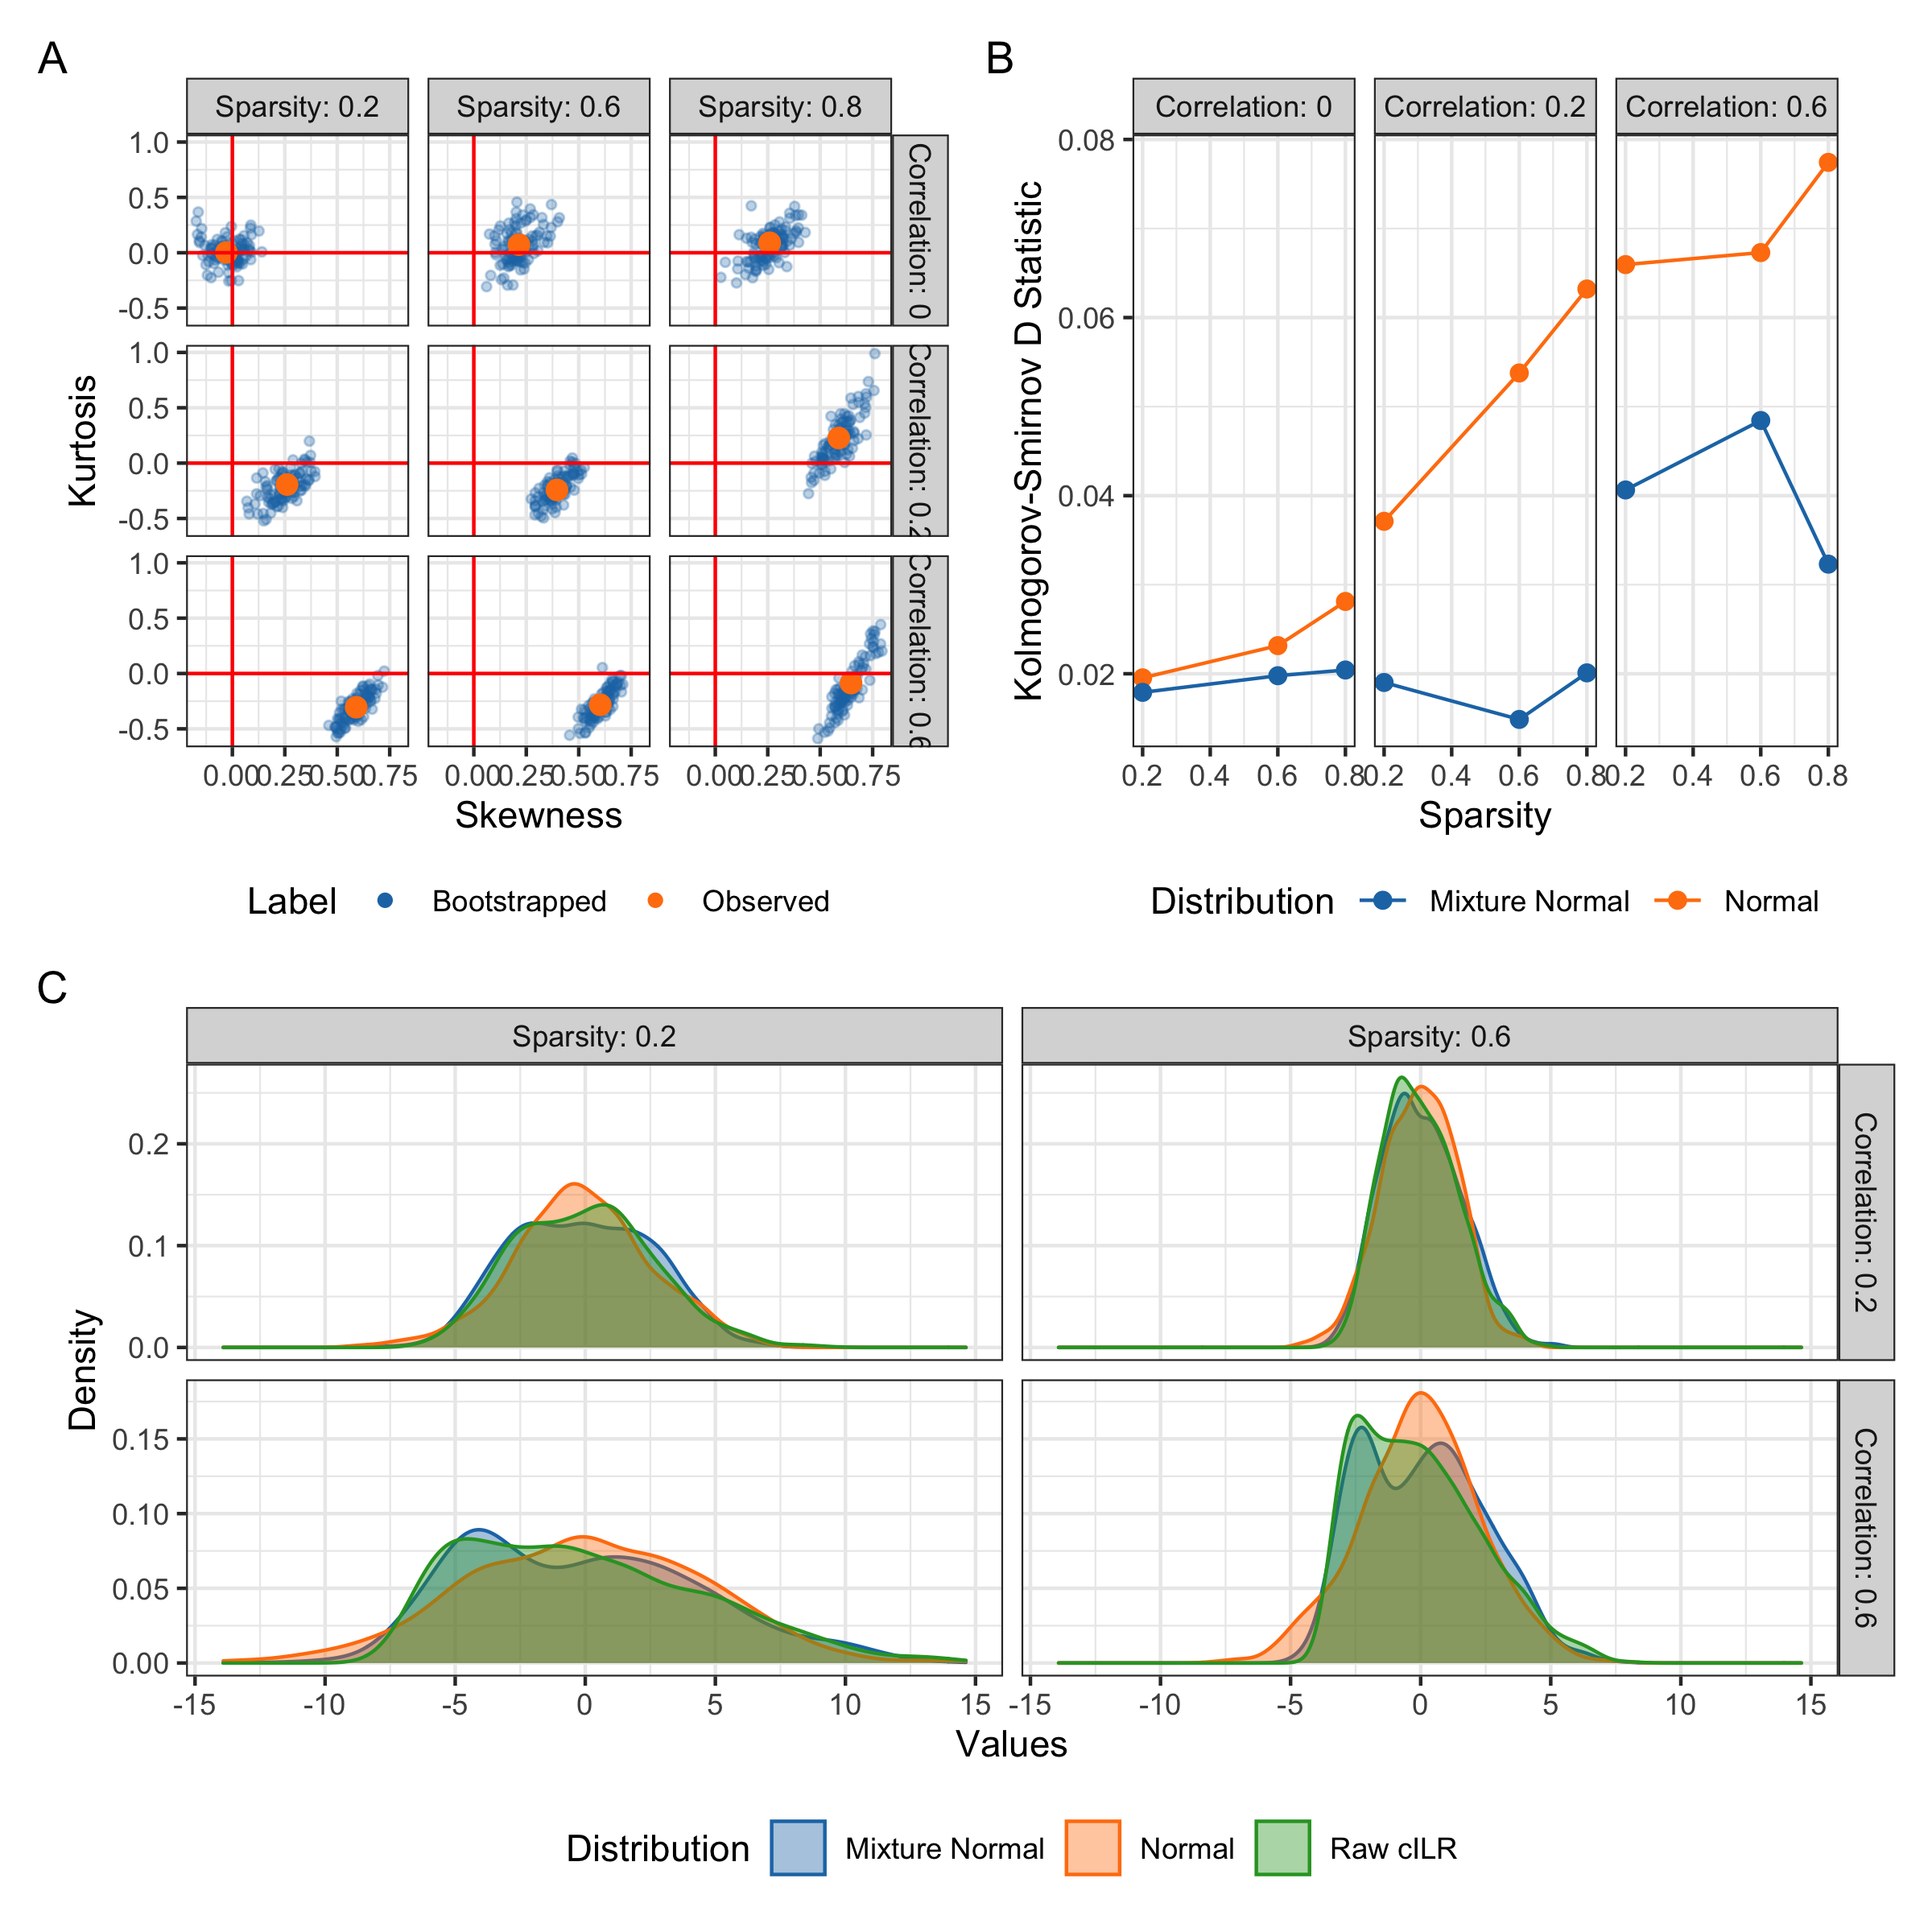
\includegraphics[width=\linewidth]{figures/kurtosis_skewness_gof.png}
    \caption{{\bf Properties of the null distribution of \DIFdelbeginFL \DIFdelFL{cILR }\DIFdelendFL \DIFaddbeginFL \DIFaddFL{CBEA }\DIFaddendFL under the global null simulations}. Panel \textbf{(B)} presents kurtosis and skewness of \DIFdelbeginFL \DIFdelFL{cILR }\DIFdelendFL \DIFaddbeginFL \DIFaddFL{CBEA }\DIFaddendFL scores while panel \textbf{(A)} presents the goodness of fit (as Kolmogorov-Smirnov D statistic) for mixture normal and normal distributions. Panel \textbf{(C)} is a density plot of the shape of the null distribution. Results indicated the necessity of estimating an empirical null and demonstrating that the mixture distribution was the better fit compared to the basic normal.}
    \label{fig:1}
\end{figure}

Additionally, the degree of kurtosis and skewness also suggests that the normal distribution itself might not be a good approximation of the null. To address this issue, we also evaluated a mixture distribution of two normal components. Panel B of Fig~\ref{fig:1} demonstrates the goodness of fit of the mixture normal and the normal distribution using Kolmogorov-Smirnov (KS) test statistic computed on fitted normal and mixture normal distribution when fitted on \DIFdelbegin \DIFdel{cILR }\DIFdelend \DIFaddbegin \DIFadd{CBEA }\DIFaddend scores in simulation scenarios under the global null. We can see that the mixture normal distribution is a better fit (lower KS scores) than the normal distribution across both sparsity and correlation settings. 

We performed our empirical null estimation by fitting our distribution of choice and computing relevant parameters on raw \DIFdelbegin \DIFdel{cILR }\DIFdelend \DIFaddbegin \DIFadd{CBEA }\DIFaddend scores on taxa-permuted data (equivalent to gene permutation in the gene expression literature). As such, the null distribution is characterized by scores computed on sets of equal size with randomly drawn taxa. However, null distribution based on taxa-permutation is sensitive to inter-taxa correlations within the set \cite{wu2012}. Since the permutation procedure does not preserve correlation structures, estimating parameters from empirical scores on permuted data will underestimate the variance inflation due to correlation. We account for this by combining the mean estimate from permuted data with the variance estimate from unpermuted data, where the inter-taxa correlation structure remains undisturbed. However, this procedure assumes that the variance of \DIFdelbegin \DIFdel{cILR }\DIFdelend \DIFaddbegin \DIFadd{CBEA }\DIFaddend is equal under both the null and alternate hypotheses. 

\subsection*{Evaluation}
All code and data sets used for evaluation of this method is publicly available and can be found on GitHub (\DIFdelbegin \href{\DIFdel{www.github.com/qpmnguyen/cILR\_analysis}}%DIFAUXCMD
%DIFDELCMD < {%%%
\DIFdelend \DIFaddbegin \href{\DIFadd{www.github.com/qpmnguyen/CBEA\_analysis}}{\DIFaddend qpmnguyen/\DIFdelbegin \DIFdel{cILR}\DIFdelend \DIFaddbegin \DIFadd{CBEA}\DIFaddend \_analysis}). 

\subsubsection*{Parametric Simulations}  
To address the performance of \DIFdelbegin \DIFdel{cILR }\DIFdelend \DIFaddbegin \DIFadd{CBEA }\DIFaddend for different modeling tasks, we simulated microbiome count data under the assumption that it follows a zero-inflated negative binomial distribution, which is a good fit for real microbiome relative abundance data \cite{calgaro2020}. Suppose $X_{ij}$ are observed counts for a sample $i$ and taxon $j$, then we have the following probability model
\begin{equation}
    \mathbf{X}_{ij} =
      \begin{cases}
        0 & \text{with probability $p_j$}\\
        \mathbf{NB}(\mu_j, \phi_j) & \text{with probability $1 - p_j$}\\
      \end{cases}       
\end{equation}

where $\mu_j$ and $\phi_j$ are mean and dispersion parameters, respectively. To incorporate a flexible correlation structure into our simulation model, we utilized the NorTA (Normal to Anything) method \cite{cario1997}. Given an $n$ by $p$ matrix of values $\mathbf{U}$ sampled from multivariate normal distribution with correlation matrix $\mathbf{\rho}$, we can generate target microbiome count vector $\mathbf{X_{.j}}$ for taxa $j$ following the marginal distribution $\mathbf{NB}$ characterized by the negative binomial cumulative distribution function $\mathbb{F_{\mathbf{NB}}}$:
\begin{equation}
    \mathbf{X}_{.j} = \mathbb{F_{\mathbf{NB}}}^{-1}(\Phi_{U_i})
\end{equation}
In this instance, for each taxon $j$, we set elements in $\mathbf{U}_{.j}$ to be zero with probability $p_j$ and applied $\mathbf{NB}^{-1}(\mu_j, \phi_j)$ on non-zero elements to generate our final count matrix $\mathbf{X}$. To ensure that our simulations match closely to real data, we fitted negative binomial distribution using a maximum likelihood approach (with the \emph{fitdistrplus} package in R \cite{delignette-muller2015}) to non-zero counts for each taxon from 16S rRNA profiling of stool samples from the Human Microbiome Project (HMP). We take the median values of the estimated mean and dispersion parameters as the baseline of our simulations. For simplicity, we assumed that inter-taxa correlation follows an exchangeable structure

\noindent \textbf{Single Sample Enrichment}: To assess type I error rate and power for enrichment significance testing at the sample level, we simulated data based on the schema above, and assessed enrichment for one focal set. Type I error was obtained under the global null as the number of samples where the null hypothesis was rejected at $\alpha = 0.05$ over the total number of samples (which represents the total number of hypotheses tested). Power was obtained using the same formulation as type I error rate but under the global alternate. We treated type I error and power as estimates of binomial proportions and utilized the Agresti-Couli \cite{agresti1998} formulation to calculate 95\% confidence intervals. Across both analyses, we varied sparsity levels ($p = 0.2, 0.4, 0.6$) and inter-taxa correlation within the set ($\rho = 0, 0.2, 0.5$). For type I error analysis, we also varied the size of the set (50, 100, 150). For power analyses, set size was kept constant at 100 but different effect sizes (fold change of 1.5, 2, and 3). All sample sizes were set at 10,000. 

For classifiability, we evaluated the scores against the true labels per sample (indicating the sample has a set with inflated counts) using the area under the receiving operator curve (AUROC/AUC). This is a strategy used in Frost \cite{frost2020a} which evaluates the informativeness of scores by assessing the relative ranking of samples (i.e. whether samples with inflated counts are highly ranked using estimated scores).  DeLong 95\% confidence intervals for AUC \cite{delong1988} were obtained for each estimate. Simulation settings for classification performance were identical to power analyses as detailed in the previous paragraph. 

\noindent \textbf{Differential Abundance Analysis}: To assess type I error rate and power for differential abundance testing task, we simulated data based on the schema above, and assessed differential abundance of 50 sets with 100 taxa per set across 20 replicates per simulation condition. Type I error is calculated as the number of differentially abundant sets over the total number of sets for each simulation under the global null. Power is defined similarly, but instead under the global alternate hypothesis. Estimates and confidence intervals for type I error and power are calculated as cross-replicate mean and standard error. A set is differentially abundant when all taxa within a set are differentially abundant with the same effect size. Across both analyses, we varied sparsity levels ($p = 0.2, 0.4, 0.6$), and inter-taxa correlation within the set ($\rho = 0, 0.2, 0.5$). Half of the sets are differentially abundant across case/control status with varying effect sizes (fold change of 1.5, 2, and 3). Due to the compositional nature of microbiome taxonomic data, simple inflation of raw counts would cause an artificial decrease in the abundance of the remaining un-inflated sets. As such, we applied a compensation procedure as described in Hawinkel et al. \cite{hawinkel2019} to ensure the validity of simulation results. All sample sizes were set at 2,000.    

\noindent \textbf{Prediction}: To assess predictive performance, we generated predictors based on the simulation schema presented above and evaluated prediction for both binary and continuous outcomes using a standard random forest model \cite{breiman2001}. For binary outcomes, we use AUC similar to the classification analyses above. For continuous outcomes, we used root mean squared error (RMSE). All predictive model fitting was performed using \emph{tidymodels} \cite{kuhn2020} suite of packages. Across both learning tasks, we varied sparsity ($p = 0.2, 0.4, 0.6$), and inter-taxa correlation ($\rho = 0, 0.2, 0.5$). Continuous outcomes $Y_{cont}$ were generated as linear combinations of taxa counts.  
\begin{equation}
    Y_{cont} = f(\mathbf{X}) + \mathbf{\epsilon}
\end{equation}
where $\mathbf{\epsilon} \sim N(0, \sigma_{\epsilon}^2)$ and $f(\mathbf{X}) = \beta_0 + \mathbf{X}\mathbf{\beta}$. For each simulation, we set $\beta_0$ to be $\frac{6}{\sqrt{10}}$ similar to \cite{xiao2018}. The degree of model saturation (the number of non zero $\mathbf{\beta}$ values) were varied between 0.1 and 0.5, and signal to noise ratio (SNR = $\frac{\sigma(f(\mathbf{X}))}{\sigma_{\epsilon}}$) was varied between 1.5, 2, and 3. 

For binary outcomes, we generate $Y_{binary}$ as Bernoulli draws with probability $p_{binary}$, where 
\begin{equation}
    p_{binary} = \frac{1}{1 + \exp(f(\mathbf{X}) + \mathbf{\epsilon})}
\end{equation}
To ensure a balance of classes, we applied the strategy described in Dong et al. \cite{dong2020} where the associated $\beta$ values are evenly split between positive and negative associations. All data sets generated from prediction tasks have 2,000 samples with 5,000 taxa over 50 sets with a size of 100 taxa per set.  

\subsubsection*{Real Datasets}

In addition to simulation analyses, we also evaluated our method using real data sets based on both 16S rRNA gene sequencing and whole-genome sequencing. All data sets are obtained from either the \emph{curatedMetagenomicData} \cite{pasolli2017} and \emph{HMP16SData} \cite{schiffer2019} R packages (2020-10-02 snapshot), or downloaded from the Qiita platform \cite{gonzalez2018}.  

\noindent \textbf{Single Sample Enrichment}: To assess the false discovery rate and true discovery rate of \DIFdelbegin \DIFdel{cILR }\DIFdelend \DIFaddbegin \DIFadd{CBEA }\DIFaddend in sample-level enrichment testing, we utilized the 16S rRNA gene sequencing of the oral microbiome at the gingival subsite from the Human Microbiome Project \cite{consortium2012, proctor2019}. We utilized this data set following the approach outlined in Calagaro et al. \cite{calgaro2020}. This data set is approximately labeled, where aerobic microbes are enriched in the supragingival subsite where the biofilm is exposed to the open air, while conversely anaerobic microbes thrive in the subgingival site \cite{thurnheer2016}. Here, we assessed the enrichment of aerobic microbes across all samples, we considered the false positive rate as the number of samples from the subgingival site with significant enrichment, and the true positive rate as the number of supragingival samples with significant enrichment. Microbial tropism annotation at the genus level was from Beghini et al. \cite{beghini2019} and was downloaded directly from the GitHub repository associated with Calagaro et al. \cite{matteocalgaro2020}. 

\noindent \textbf{Differential Abundance Analsysis}: To assess type I error using \DIFdelbegin \DIFdel{cILR }\DIFdelend \DIFaddbegin \DIFadd{CBEA }\DIFaddend scores in differential abundance analysis, we utilized the 16S rRNA gene sequencing of stool samples from the Human Microbiome Project \cite{consortium2012, proctor2019}. Here, we randomly assign samples a label of case or control, and repeated this process 500 times, assessing all candidate methods at each iteration. Type I error is then the number of taxa identified as differentially abundant across all tested taxa. For the true positive rate, we used the same gingival data set as described above. However, instead of testing for aerobic microbes as a group, the true positive rate is the number of aerobic/anaerobic genera identified as differentially abundant across all aerobic or anaerobic genera. 

\noindent \textbf{Disease Prediction}: To assess predictive power, we utilized the whole genome sequencing of stool samples of inflammatory bowel disease (IBD) patients from the MetaHIT consortium \cite{nielsen2014}. This data set contains 396 samples from a cohort of European adults, where 195 adults were classified as having IBD (which includes patients diagnosed with either ulcerative colitis or Crohn's disease). Additionally, we also utilized a similar data set from Gevers et al. \cite{gevers2014} which also profiles the gut microbiome of IBD patients and controls but using 16S rRNA gene sequencing. This data set contains 16S rRNA gene sequencing samples from a cohort of pediatric patients (ages $<$ 17) from the RISK cohort enrolled in the United States and Canada. Of the 671 samples obtained, 500 samples belong to patients with IBD. 

\subsubsection*{Comparison Methods}

\noindent \textbf{Single sample enrichment}: For type I error and power analyses, we compared the \DIFdelbegin \DIFdel{cILR }\DIFdelend \DIFaddbegin \DIFadd{CBEA }\DIFaddend method with a naive Wilcoxon rank sum test. We added a pseudocount of 1 to all values. This is a non-parametric difference in means test, where we compared the abundance of taxa of a pre-defined set and its complement within a single sample. For classification performance, we compared \DIFdelbegin \DIFdel{cILR }\DIFdelend \DIFaddbegin \DIFadd{CBEA }\DIFaddend methods against GSVA \cite{hanzelmann2013}, ssGSEA \cite{barbie2009}, and the W-statistic from the Wilcoxon rank sum test. All three approaches were applied directly on count data (after pseudocount). For GSVA, the Poisson kernel was used. 

\noindent \textbf{Differential Abundance}: Since \DIFdelbegin \DIFdel{cILR }\DIFdelend \DIFaddbegin \DIFadd{CBEA }\DIFaddend are sample-level enrichment scores, we performed differential abundance by using a Wilcoxon Rank Sum test and Welch's t-test across case/control status on \DIFdelbegin \DIFdel{cILR }\DIFdelend \DIFaddbegin \DIFadd{CBEA }\DIFaddend generated scores. We added a pseudocount of 1 to all values. For comparison, we chose representative state-of-the-art methods in differential abundance analysis, namely DESeq2 \cite{love2014,mcmurdie2014} and corncob \cite{martin2020}. For DESeq2, we performed a likelihood ratio test against an intercept only reduced model with dispersion estimated with local fit. For corncob, we also performed a likelihood ratio test against an intercept only reduced model without bootstrapping. 

\noindent \textbf{Disease Prediction}: We fit random forest on \DIFdelbegin \DIFdel{cILR }\DIFdelend \DIFaddbegin \DIFadd{CBEA }\DIFaddend scores, as well as ssGSEA \cite{hanzelmann2013} and GSVA \cite{barbie2009} similar to single sample enrichment section. We added a pseudocount of 1 to all values. Additionally, we also compared performance using \DIFdelbegin \DIFdel{cILR }\DIFdelend \DIFaddbegin \DIFadd{CBEA }\DIFaddend against a standard analysis plan where the centered log-ratio transformation (CLR) was applied to count-aggregated sets as inputs to a machine learning model. 

\section*{Results}
In this section, we present the performance of our proposed method for three applicable microbiome analysis tasks: sample level enrichment, differential abundance, and disease prediction. We obtained these results from both parametric simulations and examples from real data.  

\subsection*{Enrichment testing at the sample level}
\DIFdelbegin \DIFdel{cILR }\DIFdelend \DIFaddbegin \DIFadd{CBEA }\DIFaddend provides significance testing for enrichment at the sample level using the null distribution estimation procedure described in \nameref{methods}. Here, we present empirical results for this application of \DIFdelbegin \DIFdel{cILR }\DIFdelend \DIFaddbegin \DIFadd{CBEA }\DIFaddend assessing type I error, power, and classification capacity. 

\subsubsection*{Simulation studies}
Panel A and B in Fig~\ref{fig:2} demonstrate type I error and power respectively across different simulation conditions. We benchmarked the results of the \DIFdelbegin \DIFdel{cILR }\DIFdelend \DIFaddbegin \DIFadd{CBEA }\DIFaddend method against a naive Wilcoxon rank sum test performed at the sample level, comparing the mean count difference between taxa in the set its complement. All methods demonstrate good type I error control at $\alpha = 0.05$ under zero correlation across all simulation conditions. However, under both medium ($\rho = 0.2$) and high ($\rho = 0.5$) correlation settings, both the Wilcoxon test and unadjusted \DIFdelbegin \DIFdel{cILR }\DIFdelend \DIFaddbegin \DIFadd{CBEA }\DIFaddend variants show high levels of inflated type I error, where Wilcoxon test performed the worst. On the other hand, adjusted \DIFdelbegin \DIFdel{cILR }\DIFdelend \DIFaddbegin \DIFadd{CBEA }\DIFaddend methods (under both distributions) control for type I error at the appropriate $\alpha$ level even at high correlations. 

\begin{figure}[!h]
    \centering
    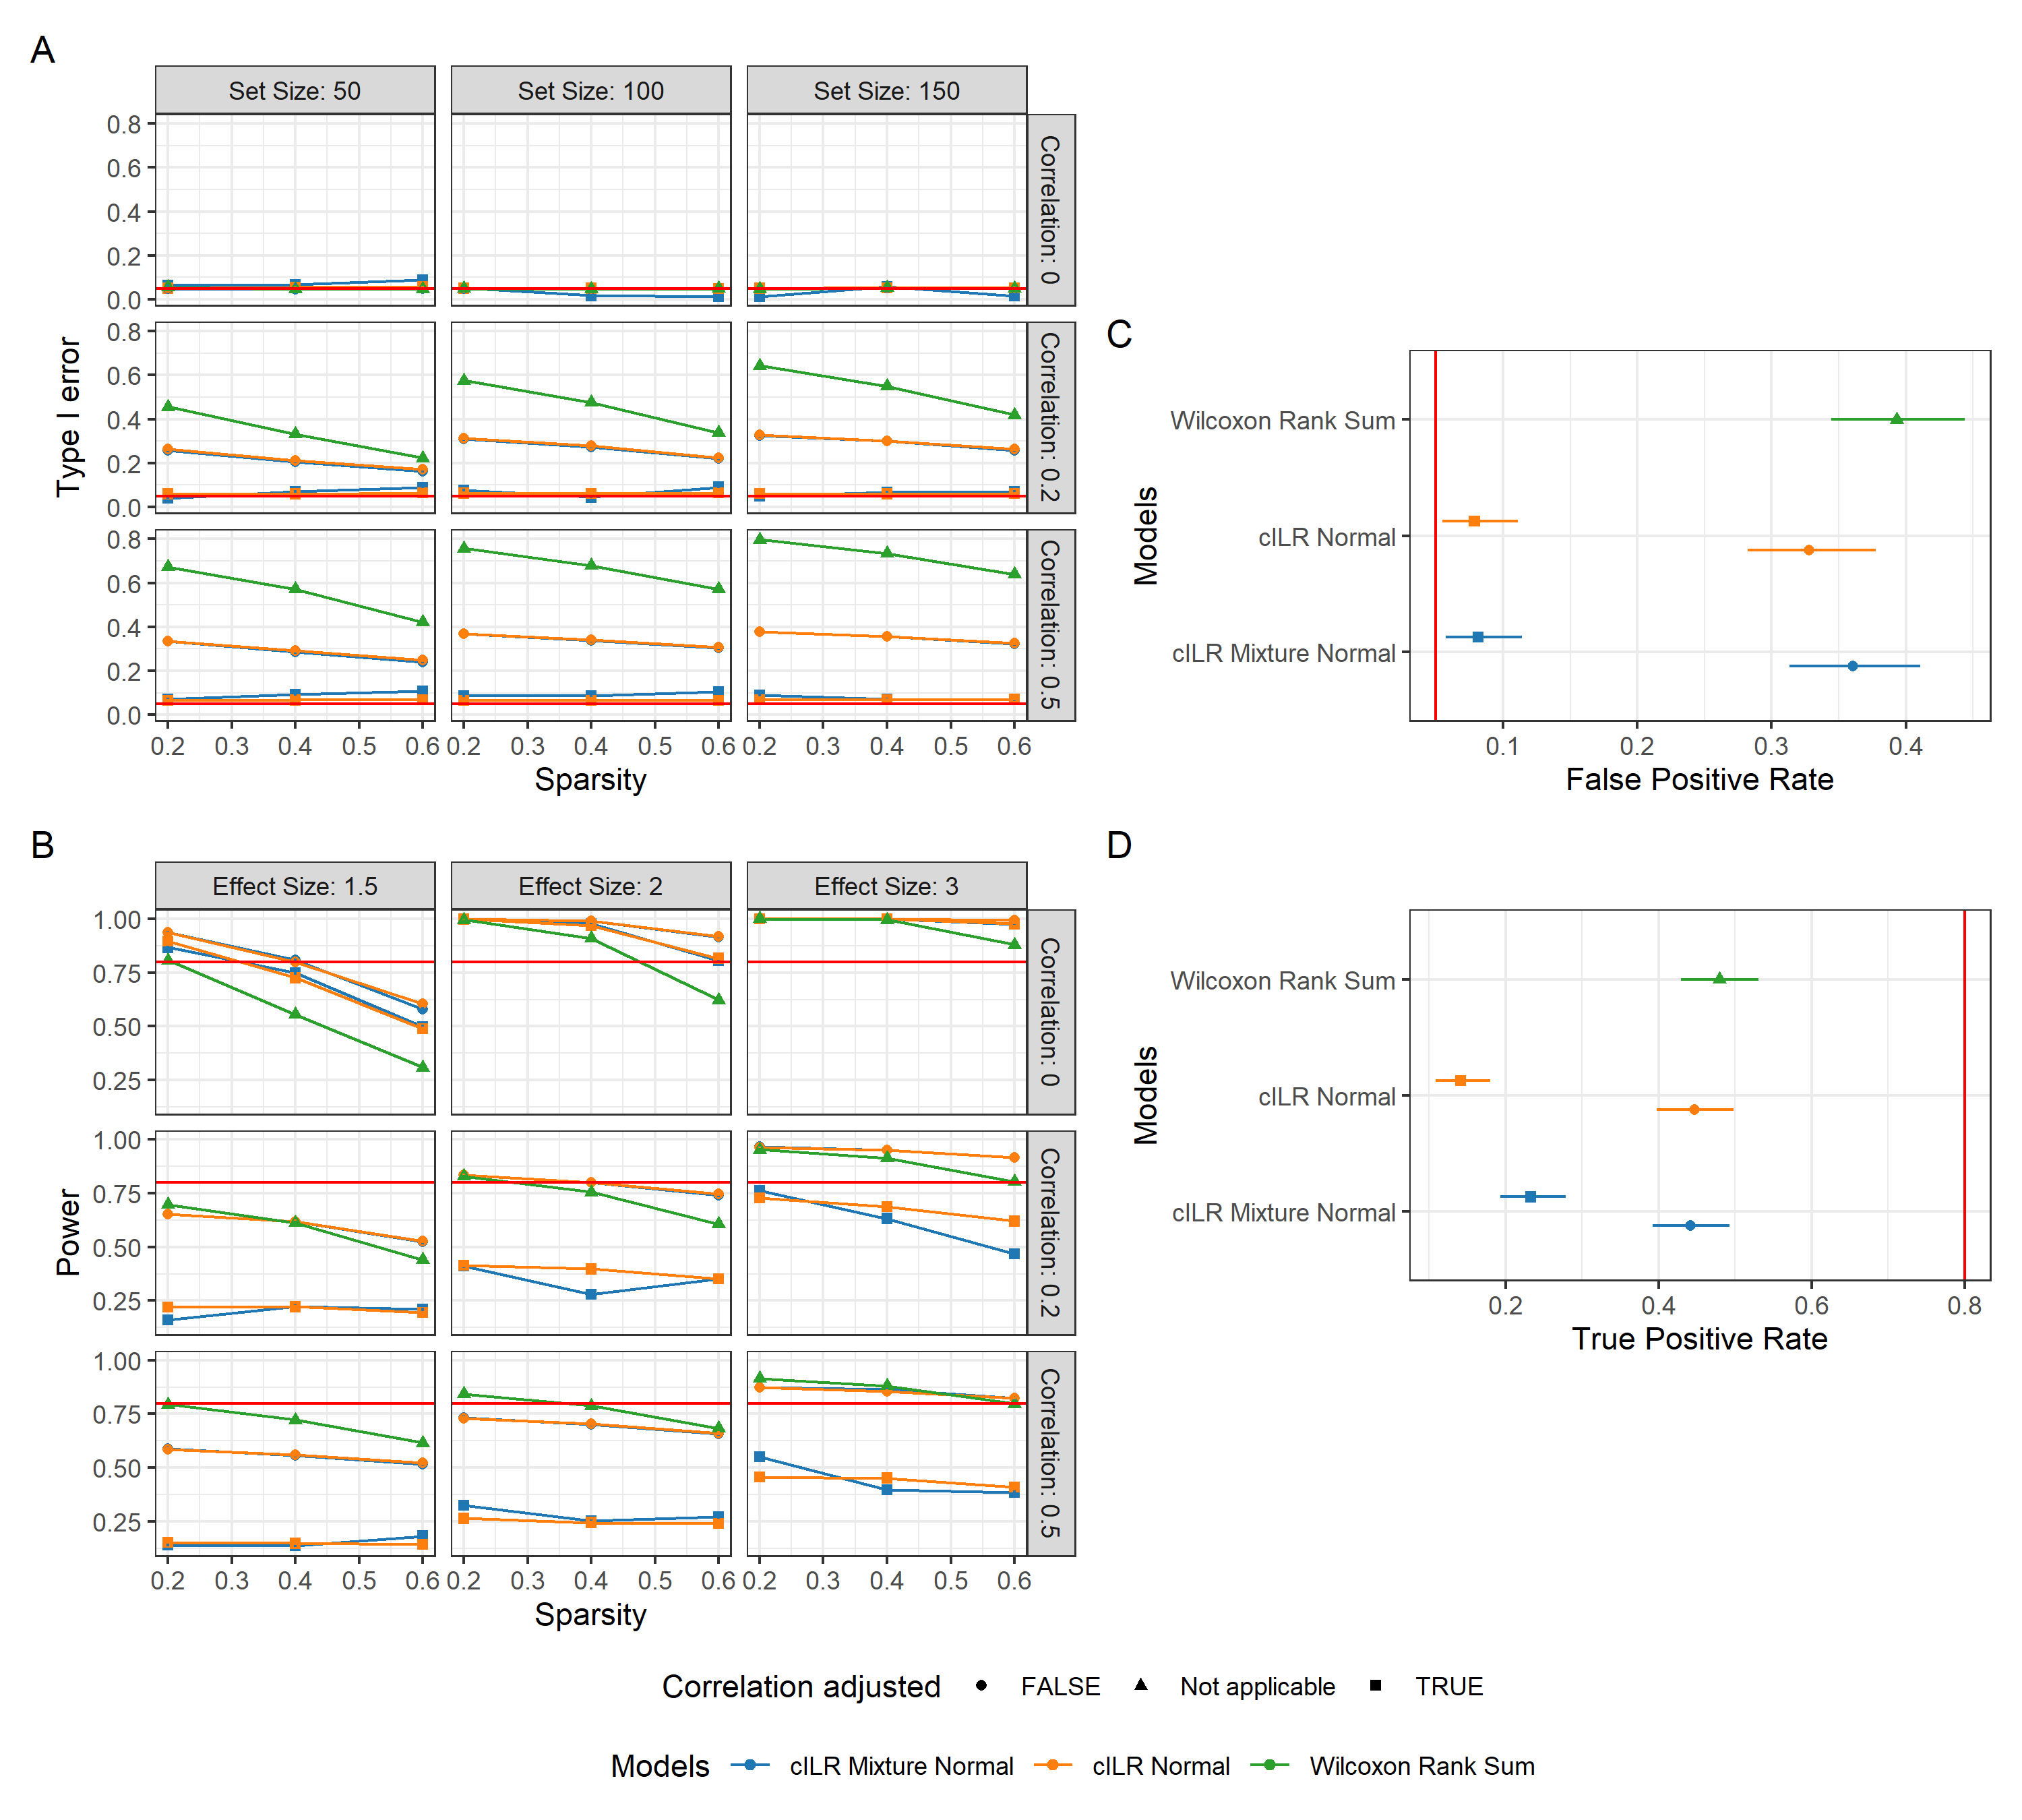
\includegraphics[width=\textwidth]{figures/sim_data_ss_hypo.png}
    \caption{Sample-level inference with \DIFdelbeginFL \DIFdelFL{cILR }\DIFdelendFL \DIFaddbeginFL \DIFaddFL{CBEA }\DIFaddendFL under parametric simulations (\textbf{(A)} and \textbf{B}), and real data analysis (\textbf{(C)} and \textbf{(D)}). In simulation analyses, panel \textbf{(A)} shows type I error rate, and panel \textbf{(B)} shows power for single sample enrichment test for a specified set and was compared against a Wilcoxon rank sum test at $\alpha$ of 0.05. In real data analysis, panel \textbf{(C)} shows the false-positive rate, and panel \textbf{(D)} shows the true positive rate. For this analysis, 16S rRNA data from the oral microbiome of the gingival site was used. The set of aerobic microbes was tested for enrichment in all samples and was identified as correctly enriched if a significant $p$-value was obtained in supragingival samples. Confidence bounds were obtained using Agresti-Couli \cite{agresti1998} approach. Adjusted \DIFdelbeginFL \DIFdelFL{cILR }\DIFdelendFL \DIFaddbeginFL \DIFaddFL{CBEA }\DIFaddendFL demonstrated control of type I error at the appropriate $\alpha$ level while remaining methods (not included in subsequent power analyses) showed an inflated type I error rate. However, this resulted in lower power for adjusted \DIFdelbeginFL \DIFdelFL{cILR }\DIFdelendFL \DIFaddbeginFL \DIFaddFL{CBEA }\DIFaddendFL methods.}
    \label{fig:2}
\end{figure}

However, the trade-off for good type I error control is demonstrably lower power, as shown in Fig~\ref{fig:2}B. In situations where there is no inter-taxa correlation, \DIFdelbegin \DIFdel{cILR }\DIFdelend \DIFaddbegin \DIFadd{CBEA }\DIFaddend still outperforms the wilcoxon rank sum test, however adjusted versions of \DIFdelbegin \DIFdel{cILR }\DIFdelend \DIFaddbegin \DIFadd{CBEA }\DIFaddend did not perform as well as un-adjusted ones. However, in higher correlation scenarios, the difference in power is much more dramatic. At the highest effect size (fold change of 3) and correlation ($\rho = 0.5$), adjusted \DIFdelbegin \DIFdel{cILR }\DIFdelend \DIFaddbegin \DIFadd{CBEA }\DIFaddend was only performing at 50\% power, while unadjusted \DIFdelbegin \DIFdel{cILR }\DIFdelend \DIFaddbegin \DIFadd{CBEA }\DIFaddend and wilcoxon rank sum test were able to reach 80\%. These results indicate that both sparsity and inter-taxa correlation impacts power, with correlation having a much more dramatic impact especially for adjusted versions of \DIFdelbegin \DIFdel{cILR}\DIFdelend \DIFaddbegin \DIFadd{CBEA}\DIFaddend . Most importantly, \DIFdelbegin \DIFdel{cILR }\DIFdelend \DIFaddbegin \DIFadd{CBEA }\DIFaddend demonstrate higher power in all scenarios where type I error is properly controlled.    

To further assess the utility of \DIFdelbegin \DIFdel{cILR }\DIFdelend \DIFaddbegin \DIFadd{CBEA }\DIFaddend in classifying samples with enriched sets, we generated AUC scores for different \DIFdelbegin \DIFdel{cILR }\DIFdelend \DIFaddbegin \DIFadd{CBEA }\DIFaddend scores using true labels of whether a sample has an inflated set. This analysis, therefore, assessed the relative ranking of samples using \DIFdelbegin \DIFdel{cILR }\DIFdelend \DIFaddbegin \DIFadd{CBEA }\DIFaddend scores whereby high scores should correspond to samples that are known to be inflated. Fig~\ref{fig:3} presents this result. We compared different variants of \DIFdelbegin \DIFdel{cILR }\DIFdelend \DIFaddbegin \DIFadd{CBEA }\DIFaddend against competing methods in the gene set testing space (GSVA \cite{hanzelmann2013} and ssGSEA \cite{barbie2009}), as well as the $W$ test statistic from the Wilcoxon rank sum test. Across both simulations (Fig~\ref{fig:3}A) and real-data applications (Fig~\ref{fig:3}B), \DIFdelbegin \DIFdel{cILR }\DIFdelend \DIFaddbegin \DIFadd{CBEA }\DIFaddend scores perform marginally better especially in low effect size situations but did not stand out in most other scenarios. In simulation studies, classification performance was good (around AUC of 0.8) even at high correlation settings, only requiring medium effect sizes (fold change of 2). Notably, the W-statistic provided the least information for classifying samples with inflated taxa.

\subsubsection*{Real data evaluations}  
These observations were replicated when assessed on the semi-labeled gingival data set from the Human Microbiome Project as described in \nameref{methods}. Here, we tested the enrichment of aerobic microbes for each sample using approaches similar to our parametric simulations. As expected in Fig~\ref{fig:2}C, the proportion of falsely rejected hypotheses was high in the naive Wilcoxon test and unadjusted \DIFdelbegin \DIFdel{cILR }\DIFdelend \DIFaddbegin \DIFadd{CBEA }\DIFaddend methods. Conversely, adjusted \DIFdelbegin \DIFdel{cILR }\DIFdelend \DIFaddbegin \DIFadd{CBEA }\DIFaddend controls for false positives adequately at the correct $\alpha$ level of 0.05. Power analysis (Fig~\ref{fig:2}D) showed similar patterns, where unadjusted \DIFdelbegin \DIFdel{cILR }\DIFdelend \DIFaddbegin \DIFadd{CBEA }\DIFaddend methods and the Wilcoxon test have a higher proportion of null hypotheses correctly rejected, however, these results are not useful to a practitioner as the number of falsely rejected hypotheses are also equally high.  

\begin{figure}[!h]
    \centering
    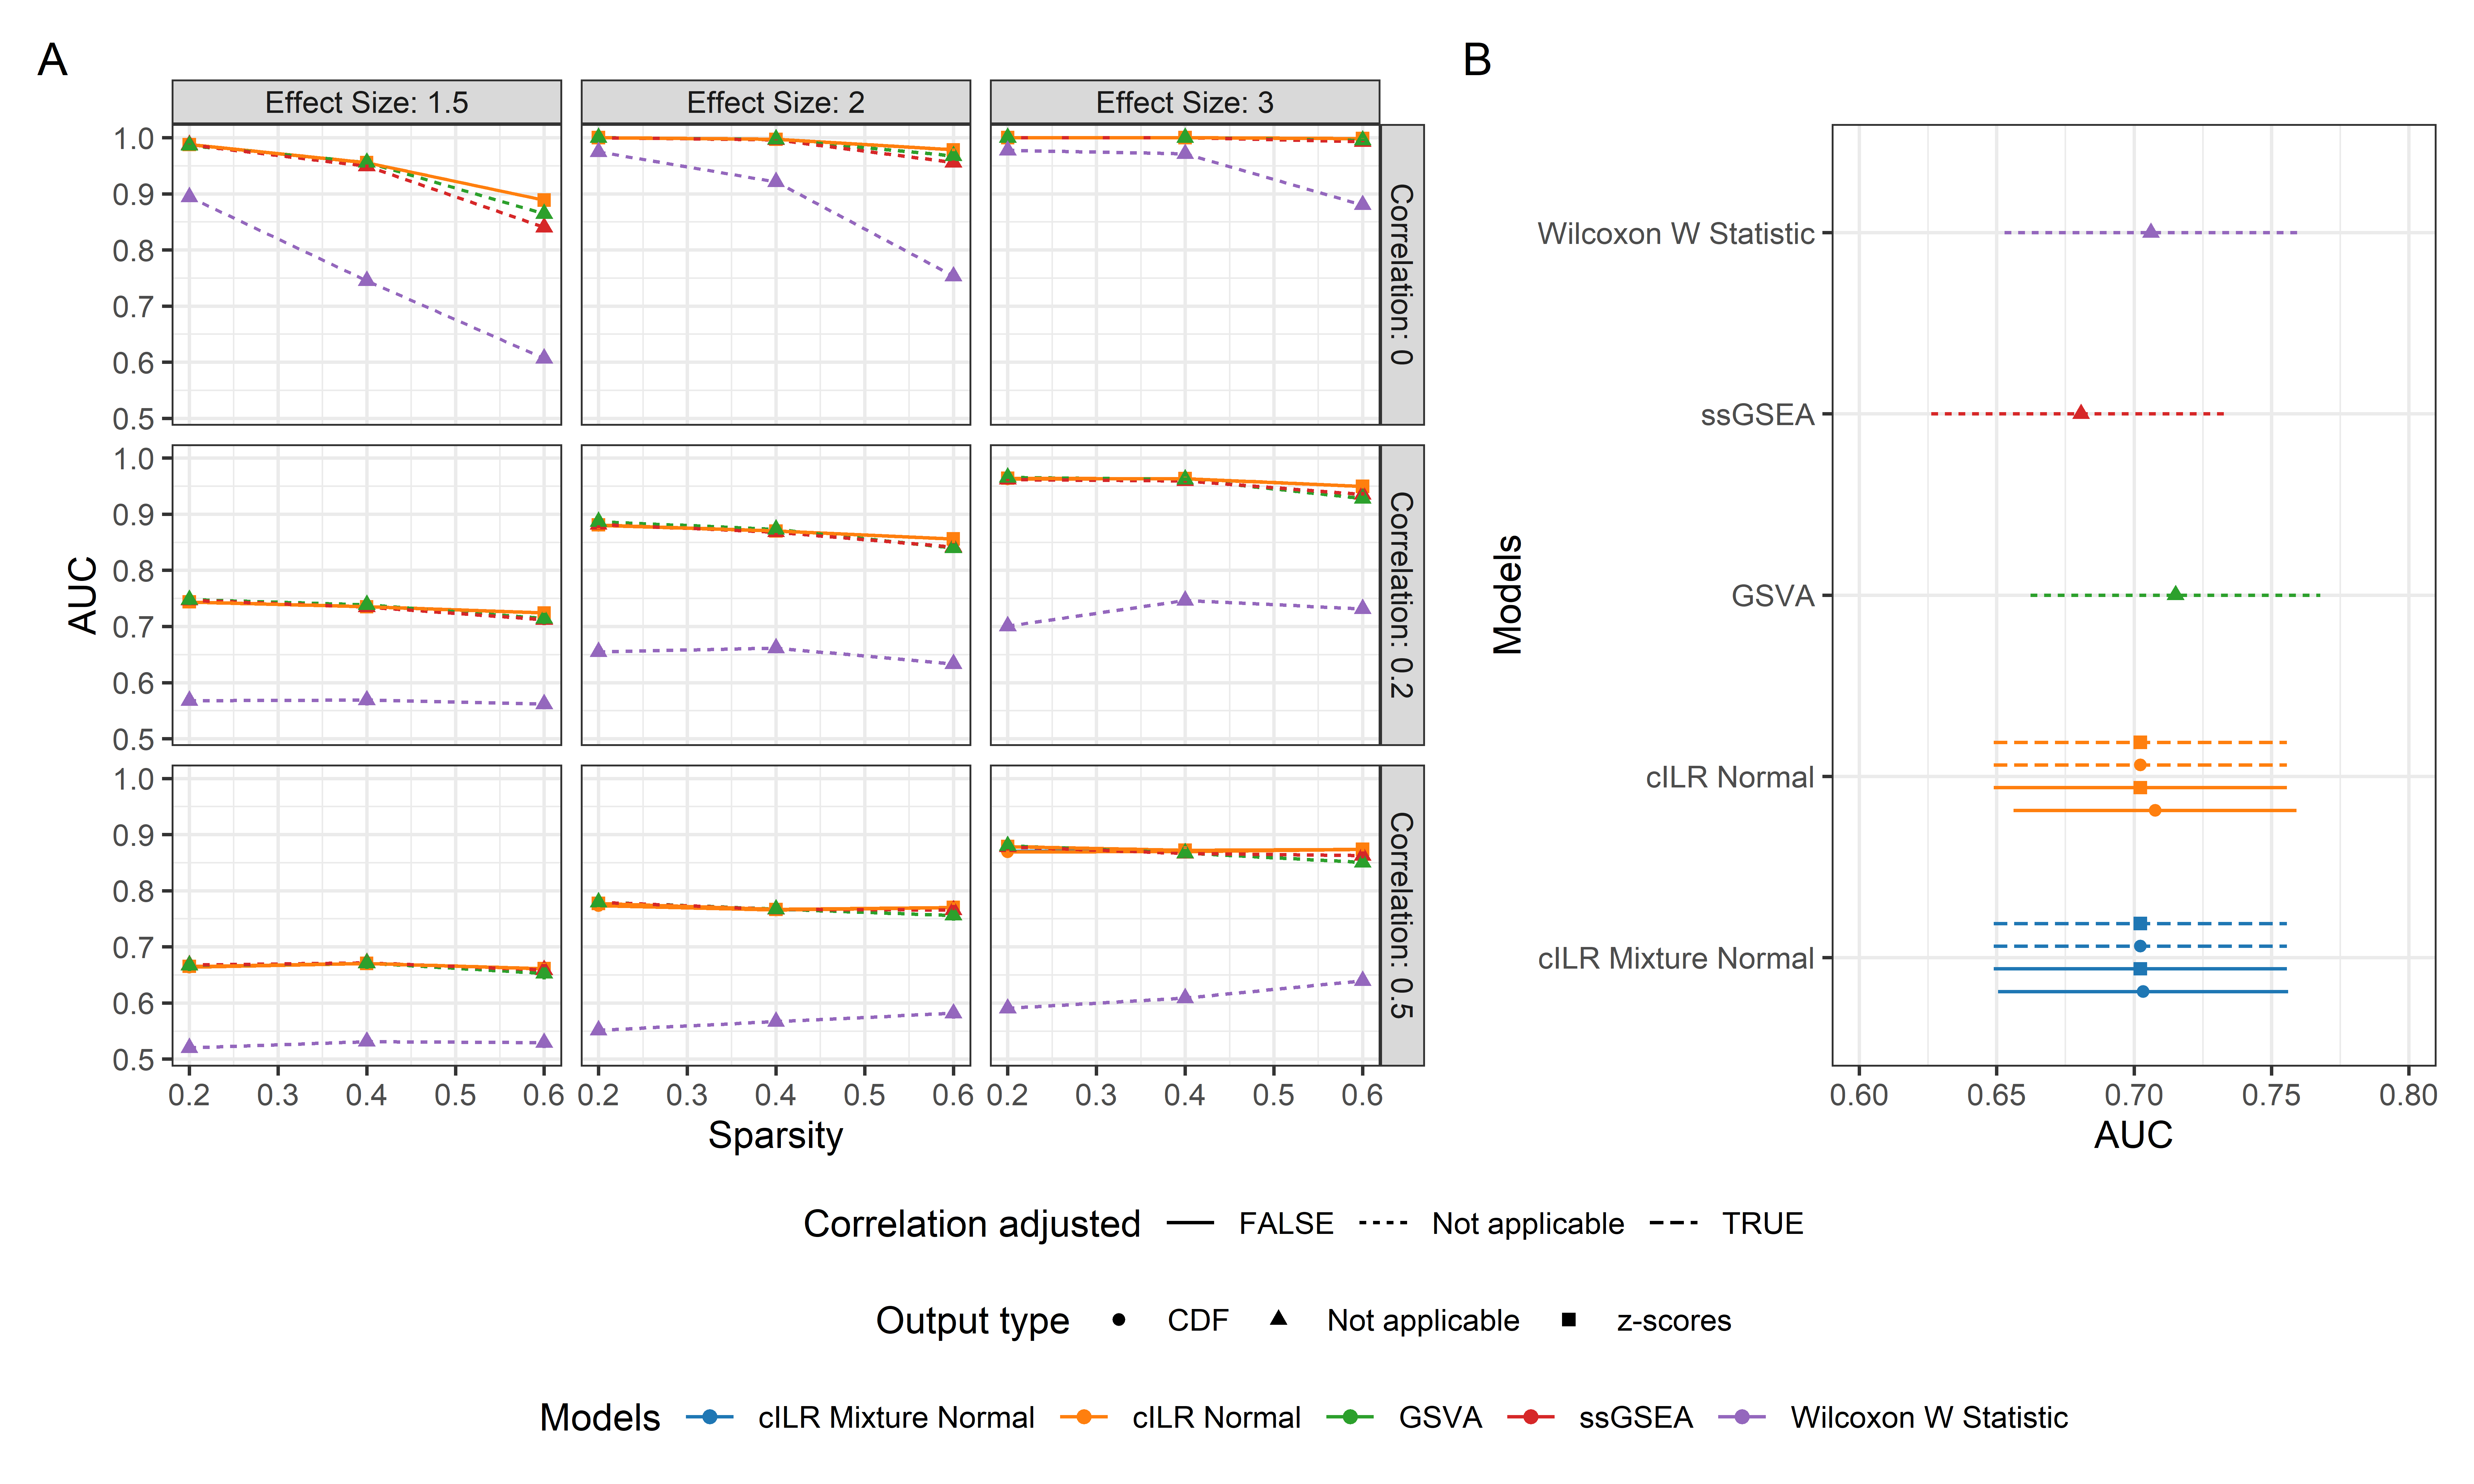
\includegraphics[width = \textwidth]{figures/sim_data_ss_auc.png}
    \caption{Classification performance via AUC of \DIFdelbeginFL \DIFdelFL{cILR}\DIFdelendFL \DIFaddbeginFL \DIFaddFL{CBEA}\DIFaddendFL , ssGSEA, GSVA, and Wilcoxon $U$ statistic on simulated data \textbf{(A)} the gingival data set from the Human Microbiome Project  \textbf{(B)} as detailed in \nameref{methods}. Performance scores measure whether scores can highly rank samples that are known to have inflated abundance. In the gingival data set presented in panel \textbf{(B)}, samples from the supragingival site are assumed to have an inflated abundance of aerobic microbes. Error bars are the 95\% DeLong confidence intervals for AUC \cite{delong1988}} 
    \label{fig:3}
\end{figure}

\subsection*{Differential abundance analysis}
\DIFdelbegin \DIFdel{cILR }\DIFdelend \DIFaddbegin \DIFadd{CBEA }\DIFaddend generates sample-specific scores representing the degree of enrichment of a pre-defined set. As such, we want to assess the ability to use these scores for differential abundance analysis in combination with a standard difference of means statistical test (Welch's t-test and Wilcoxon rank sum test). We compared the performance of this approach with \DIFdelbegin \DIFdel{cILR }\DIFdelend \DIFaddbegin \DIFadd{CBEA }\DIFaddend and two commonly used methods for differential abundance testing in the microbiome literature: DESeq2 \cite{love2014} and corncob \cite{martin2020}.   

\subsubsection*{Simulation studies}
\begin{figure}[!h]
    \centering
    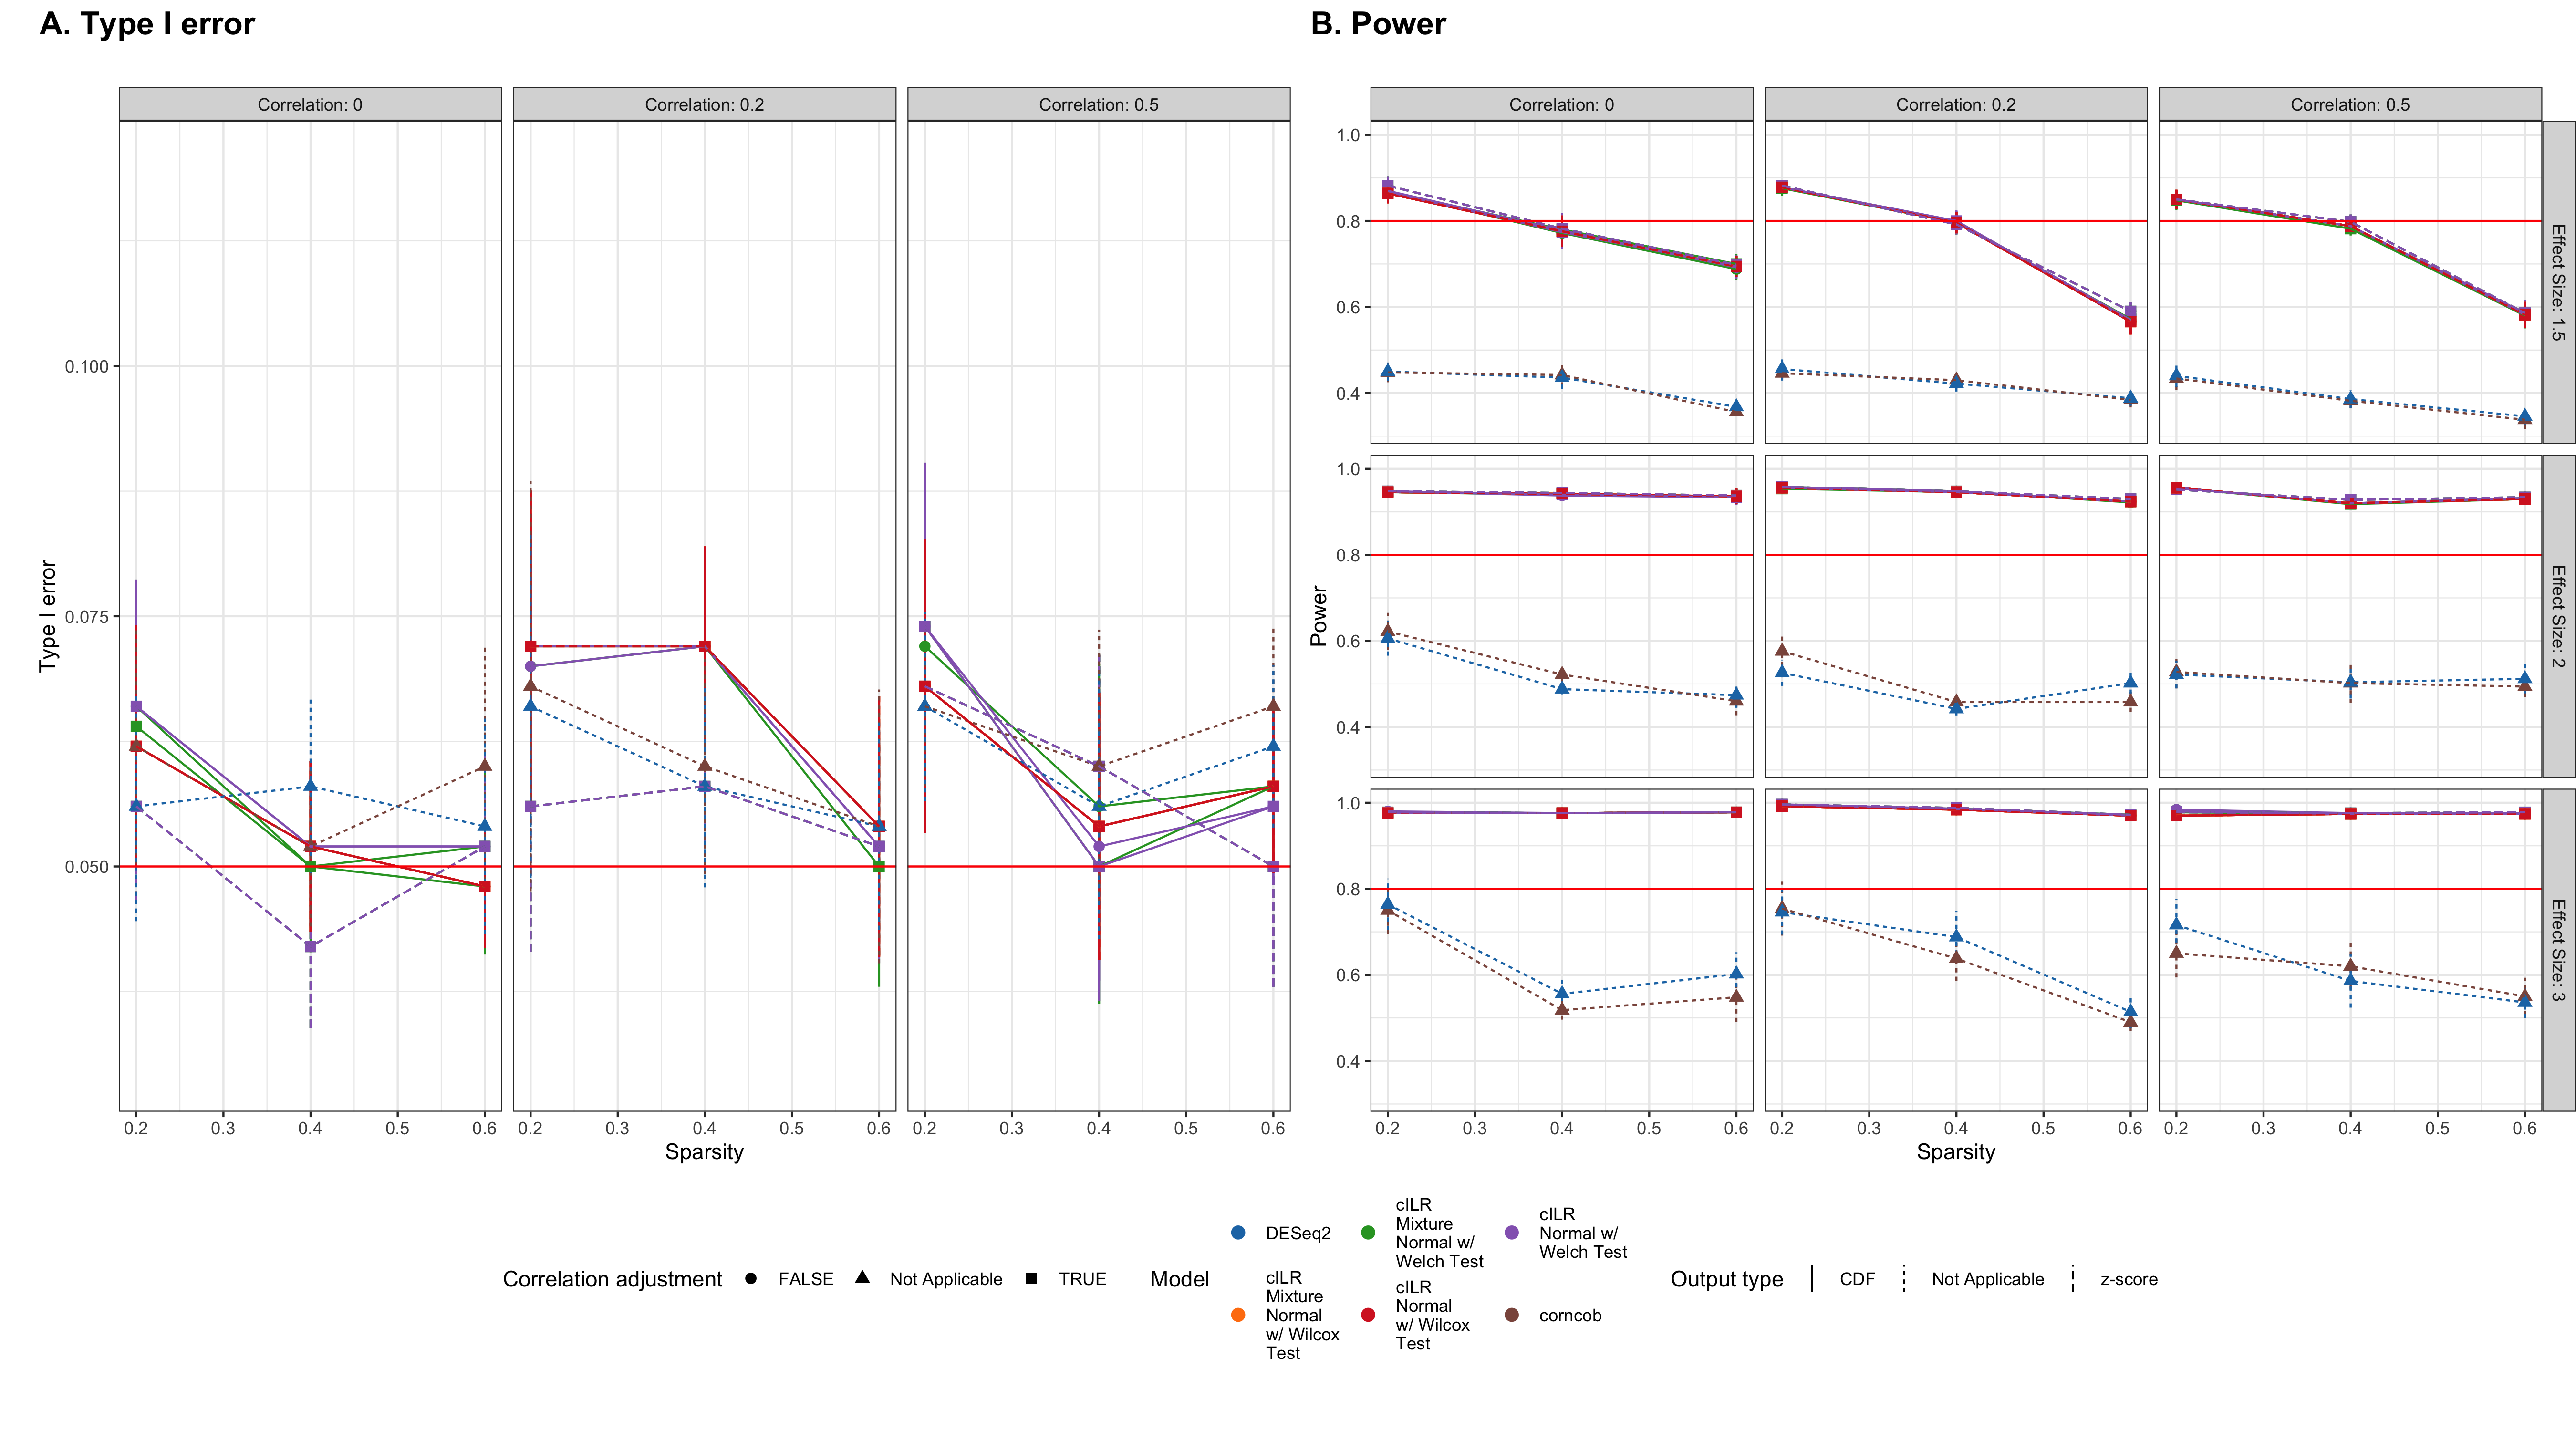
\includegraphics[width = \textwidth]{figures/sim_diff_ab_comb.png}
    \caption{Type I error rate \textbf{(A)} and power \textbf{(B)} for differential abundance test across different parametric simulation scenarios. For \DIFdelbeginFL \DIFdelFL{cILR }\DIFdelendFL \DIFaddbeginFL \DIFaddFL{CBEA }\DIFaddendFL methods, differential abundance analysis was performed using a difference in means test (either Wilcoxon rank-sum test or Welch's t-test) across case/control status using single sample scores generated by \DIFdelbeginFL \DIFdelFL{cILR }\DIFdelendFL \DIFaddbeginFL \DIFaddFL{CBEA }\DIFaddendFL (across different output types and distributional assumptions). \DIFdelbeginFL \DIFdelFL{cILR }\DIFdelendFL \DIFaddbeginFL \DIFaddFL{CBEA }\DIFaddendFL associated methods demonstrated similar type I error to conventional differential abundance analysis methods but with more power to detect differences even at small effect sizes.} 
    \label{fig:4}
\end{figure}

Fig.~\ref{fig:4} present results for simulation studies for both type I error (panel A) and power (panel B) evaluations. All methods control for type I error well across both sparsity and correlation levels, where the estimated rate was consistently around the 0.05 pre-defined threshold. Results were similar across all evaluated methods, although in some instances, for example in medium correlation setting ($\rho = 0.2$), the unadjusted \DIFdelbegin \DIFdel{cILR }\DIFdelend \DIFaddbegin \DIFadd{CBEA }\DIFaddend resulted in higher type I error, regardless of difference in means test and distribution of choice. 

The difference between the methods is more noticeable when evaluating power. All \DIFdelbegin \DIFdel{cILR }\DIFdelend \DIFaddbegin \DIFadd{CBEA }\DIFaddend associated variants showed much higher power even when the effect size is limited (fold change is 1.5), and there is a noticeable gap in performance between \DIFdelbegin \DIFdel{cILR }\DIFdelend \DIFaddbegin \DIFadd{CBEA }\DIFaddend and both DESeq2 and corncob. Surprisingly, this effect is consistent across correlation levels and sparsity, even though we expectedly see performance in power drop as a function of sparsity especially in low effect size settings.  

\subsubsection*{Real data evaluations}
In addition to simulation studies, we also evaluated performance of the methods on real 16S rRNA gene sequencing data set from HMP (Fig~\ref{fig:5}). For type I error evaluations, we use stool samples and randomly assign them with case/control status and calculated type I error as the proportion of genera identified as significantly different. For true positive rate evaluations, we use the gingival data set as detailed in the previous section, and calculated the true positive rate as the proportion of genera labeled as either anaerobic or aerobic that were found to be significant.   

We observed both corncob and DESeq2 had significantly inflated type I error rate while all variations of \DIFdelbegin \DIFdel{cILR }\DIFdelend \DIFaddbegin \DIFadd{CBEA }\DIFaddend were controlling for type I error at the defined $\alpha$ threshold of 0.05. This is surprising given the consistency of preserving type I error for both corncob and DESeq2 in all simulation evaluations. 

In true positive experiments with data from the gingival site, estimated rates were more similar across the different methods. As expected, using the Wilcoxon rank sum test resulted in lower true positive rate compared to remaining methods, but the difference was not noticable. This is also surprising given that in simulation studies, both corncob and DESeq2 showed markedly lower power across all effect sizes.  

\begin{figure}[!h]
    \centering
    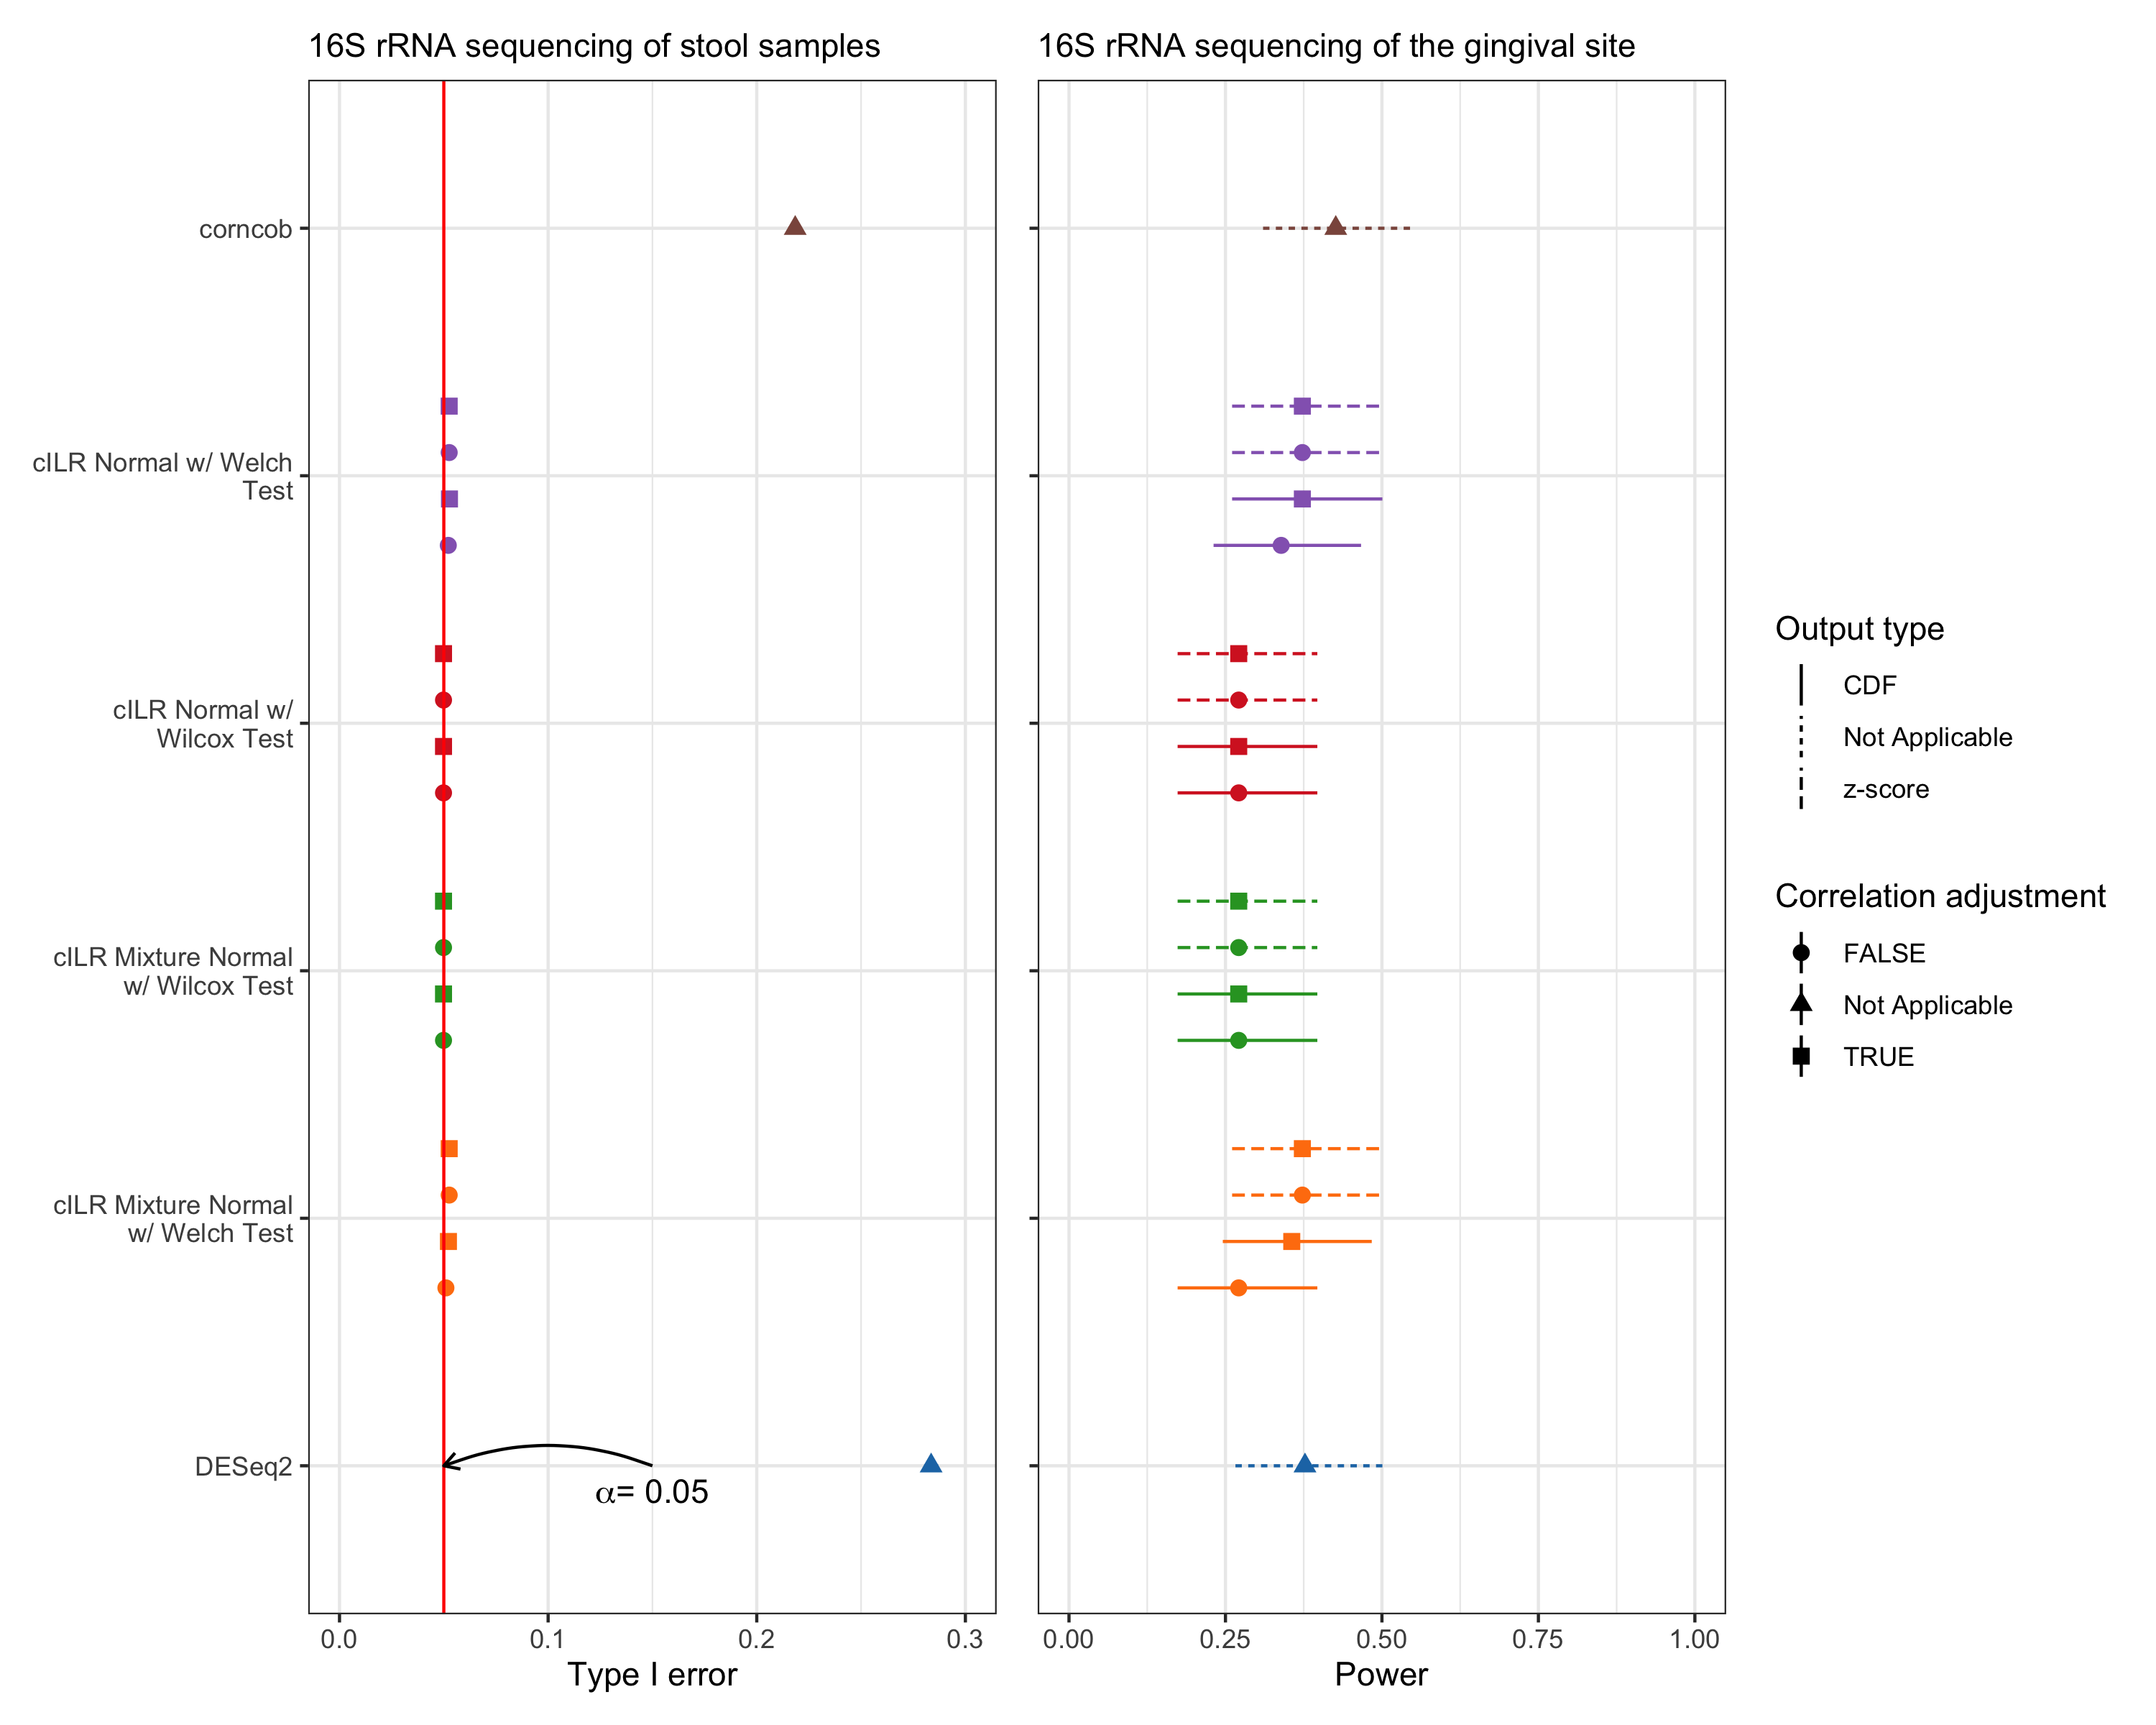
\includegraphics[width = \textwidth]{figures/data_diff_ab.png}
    \caption{Differential abundance analysis using corncob, DESeq2 and \DIFdelbeginFL \DIFdelFL{cILR }\DIFdelendFL \DIFaddbeginFL \DIFaddFL{CBEA }\DIFaddendFL with either Wilcoxon rank sum test or Welch's t-test. Panel \textbf{(A)} shows type I error results as the proportion of significant genera after 500 iterations where case/control status was assigned randomly to each sample. Panel \textbf{(B)} shows true positive rate results as the proportion of significant genera who are either obligate anaerobes or aerobes. Both evaluations use 16S rRNA gene sequencing data from HMP. Type I error evaluation used stool samples while the true positive rate evaluation used samples from the gingival site. Results showed that \DIFdelbeginFL \DIFdelFL{cILR }\DIFdelendFL \DIFaddbeginFL \DIFaddFL{CBEA }\DIFaddendFL associated methods were able to keep type I error rate at approximately 0.05 while still demonstrating similar power as both corncob and DESeq2} 
    \label{fig:5}
\end{figure}

\subsection*{Disease Prediction}   
Since \DIFdelbegin \DIFdel{cILR }\DIFdelend \DIFaddbegin \DIFadd{CBEA }\DIFaddend can generate informative scores that can discriminate between samples with inflated counts for a set (Fig~\ref{fig:2}), we want to assess whether they can also act as useful inputs to predictive models. In this section we assessed the predictive performance of a naive random forest model \cite{breiman2001} with different single sample enrichment scoring methods as inputs (evaluating \DIFdelbegin \DIFdel{cILR}\DIFdelend \DIFaddbegin \DIFadd{CBEA}\DIFaddend , ssGSEA, and GSVA). Additionally, we also compared predictive performance of using these scores against the a standard approach of using the centered log ratio transformation (CLR) on taxon sets aggregated via abundance summations.     
\subsubsection*{Simulation studies}
Fig~\ref{fig:6} shows results for simulation studies as detailed in the \nameref{methods} section. Panel A presents results for a regression learning task with a continuous outcome while panel B presents results for a classification task with a binary outcome. As expected, performance across all assessed methods increased with a higher signal-to-noise ratio. Both CLR and \DIFdelbegin \DIFdel{cILR }\DIFdelend \DIFaddbegin \DIFadd{CBEA }\DIFaddend approaches outperformed both GSVA and ssGSEA across all simulation conditions and learning tasks. This is because both GSVA and ssGSEA are more sensitive to the degree of inter-taxa correlation and sparsity, while \DIFdelbegin \DIFdel{cILR }\DIFdelend \DIFaddbegin \DIFadd{CBEA }\DIFaddend and CLR did not experience a similar level of impact. As such, performance gap widens with increasing correlation and sparsity. Interestingly, this difference in performance is not as pronounced under high levels of effect saturation (across both learning tasks), suggesting that when there is a high number of sets contributing to an effect, model choice might not be as important.   

In this analysis, \DIFdelbegin \DIFdel{cILR }\DIFdelend \DIFaddbegin \DIFadd{CBEA }\DIFaddend unfortunately did not outperform the CLR approach, which is standard practice within the microbiome literature \cite{gloor2017}. This difference in performance is more notable in regression learning tasks compared to classification, and at lower levels of effect saturation. However, the degree of separation between the two approaches is not as dramatic as between GSVA/ssGSEA and \DIFdelbegin \DIFdel{cILR}\DIFdelend \DIFaddbegin \DIFadd{CBEA}\DIFaddend /CLR. Moreover, the performance gap decreases with increasing effect signal-to-noise ratio and sparsity. Additionally, we did not observe any performance difference between the different variations of \DIFdelbegin \DIFdel{cILR}\DIFdelend \DIFaddbegin \DIFadd{CBEA}\DIFaddend . 

\begin{figure}[!h]
    \centering
    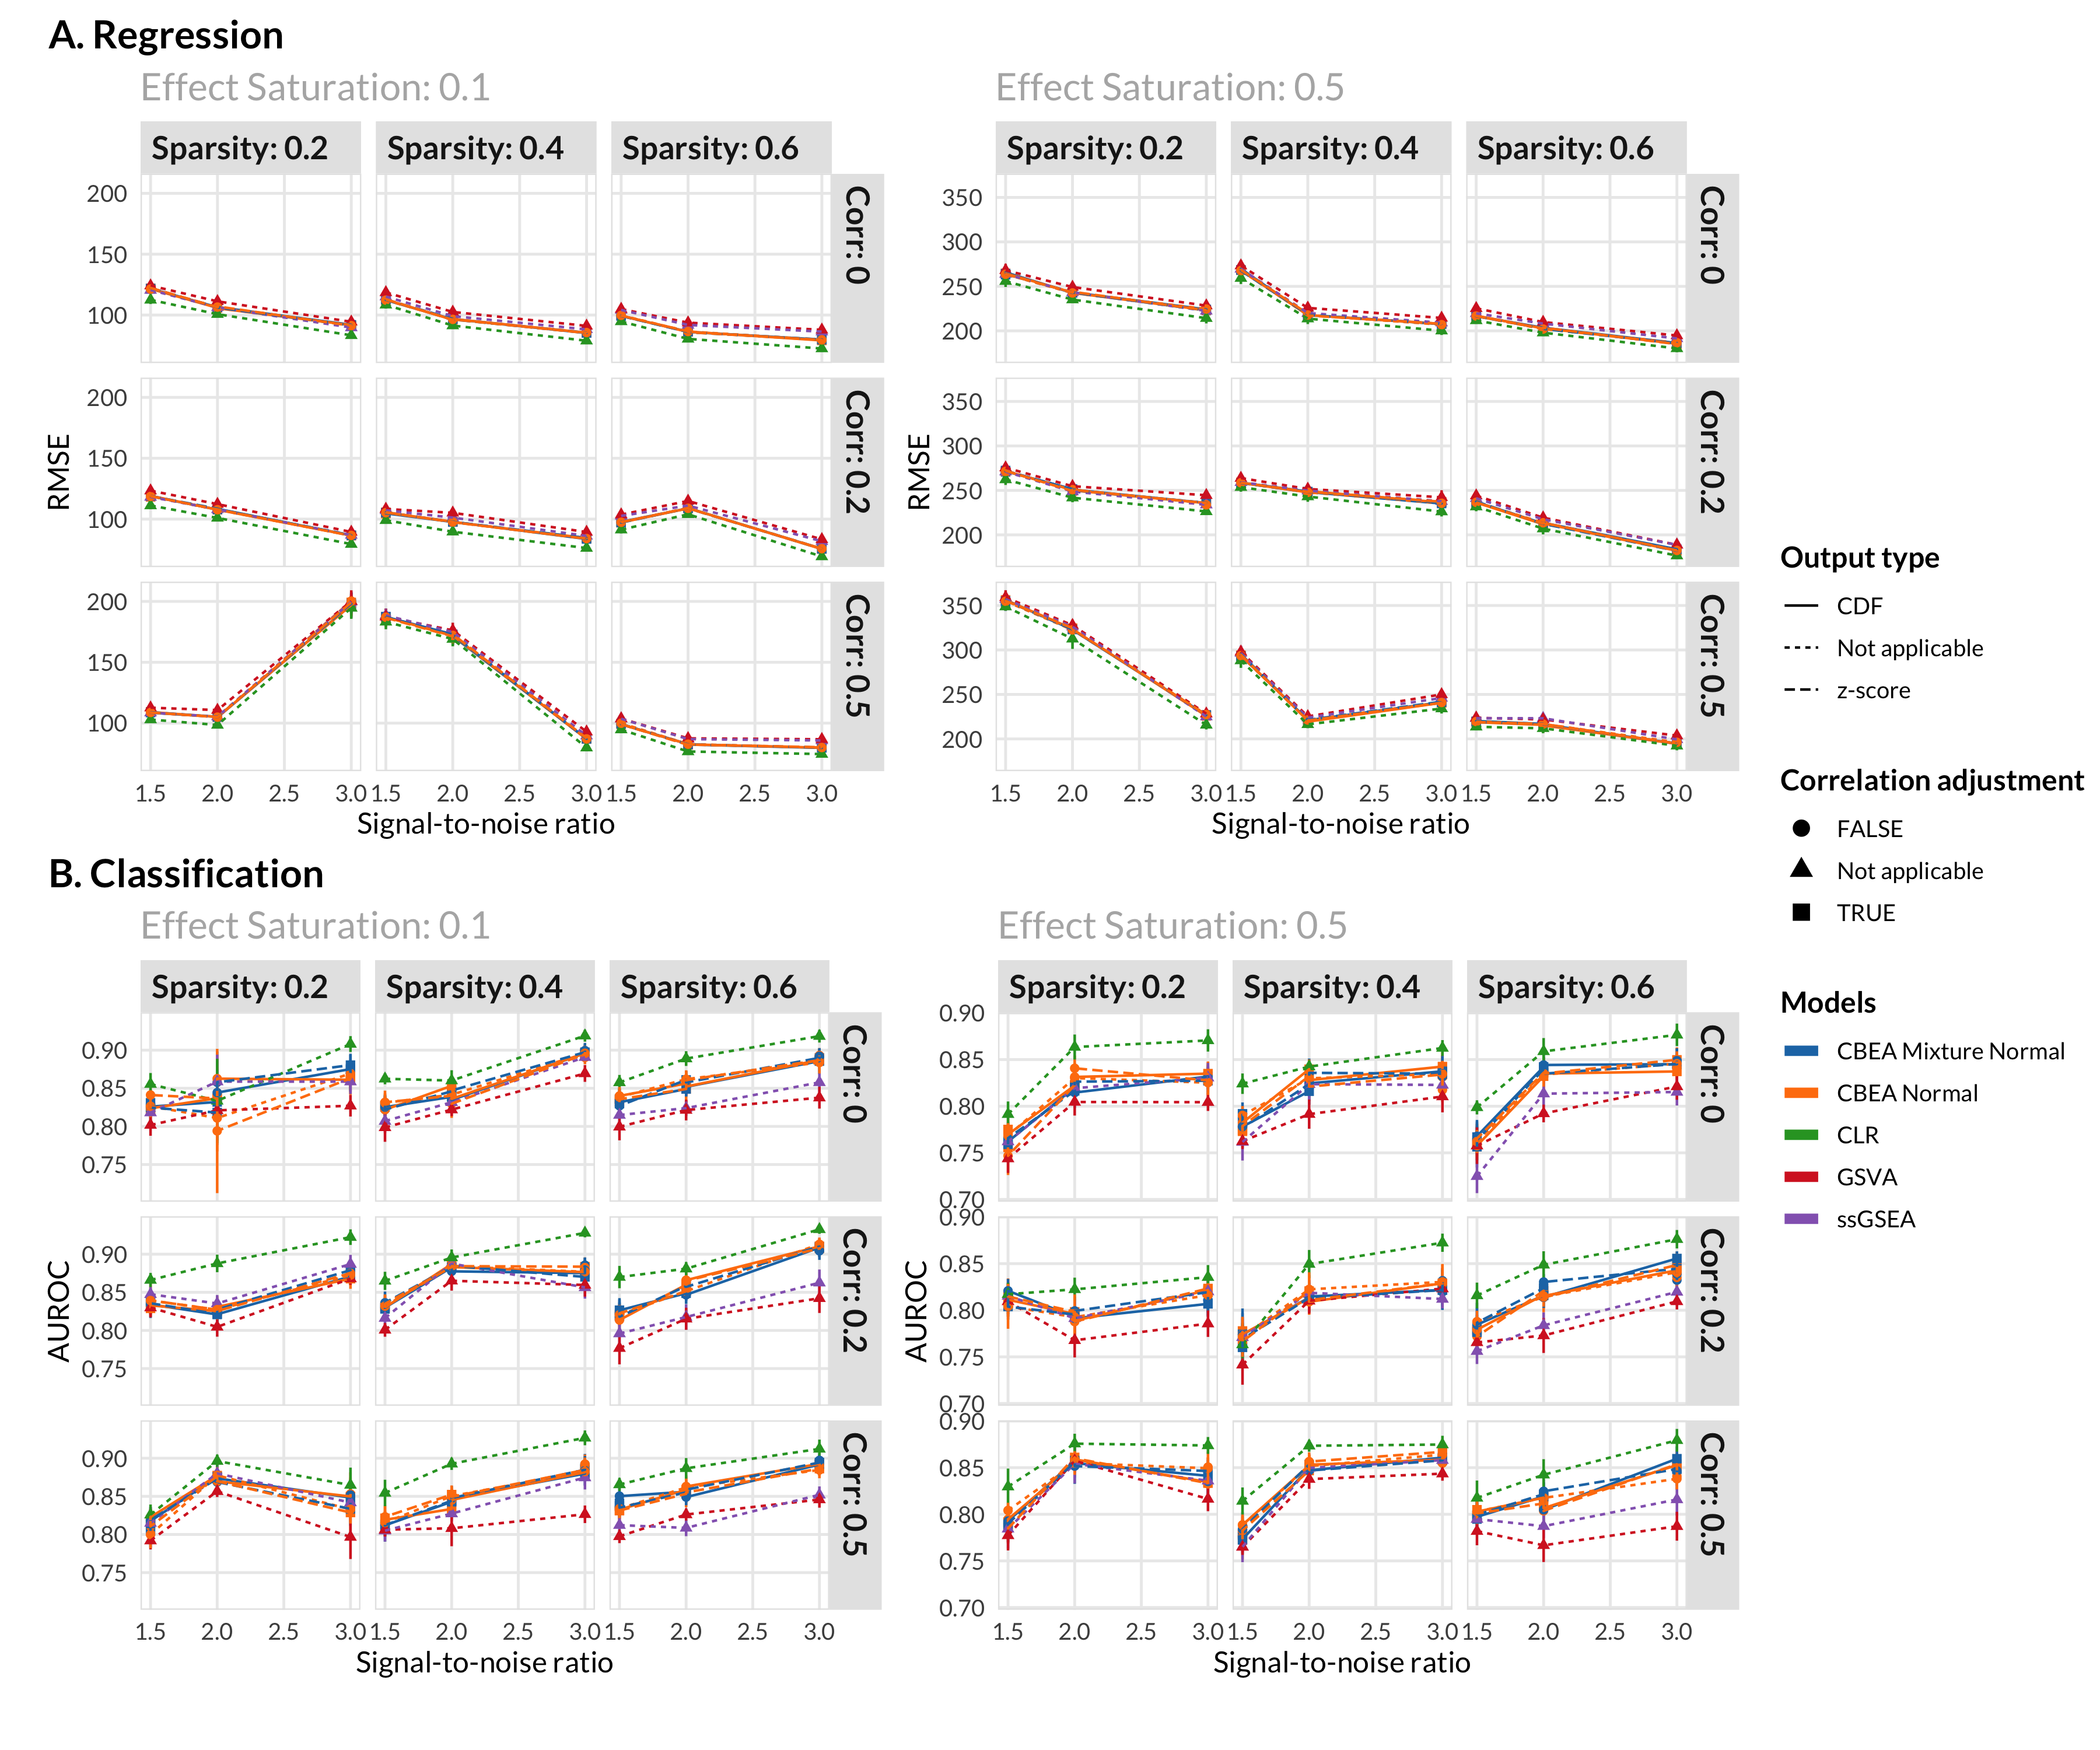
\includegraphics[width = \linewidth]{figures/sim_pred_combined.png}
    \caption{Predictive performance of a naive random forest model trained on \DIFdelbeginFL \DIFdelFL{cILR}\DIFdelendFL \DIFaddbeginFL \DIFaddFL{CBEA}\DIFaddendFL , ssGSEA, GSVA generated scores as well as the standard CLR approach on simulated across different levels of data sparsity, inter-taxa correlation, effect saturation, and signal-to-noise ratio. Panel \textbf{(A)} presents performance on a regression task using predictive R-squared as the evaluation measure. Panel \textbf{(B)} presents performance on a classification task with AUC as the evaluation measure. \DIFdelbeginFL \DIFdelFL{cILR }\DIFdelendFL \DIFaddbeginFL \DIFaddFL{CBEA }\DIFaddendFL approaches outperformed GSVA and ssGSEA across all simulation conditions but not the CLR approach.}
    \label{fig:6}
\end{figure}


%\begin{figure}[!ht]
%    \centering
%    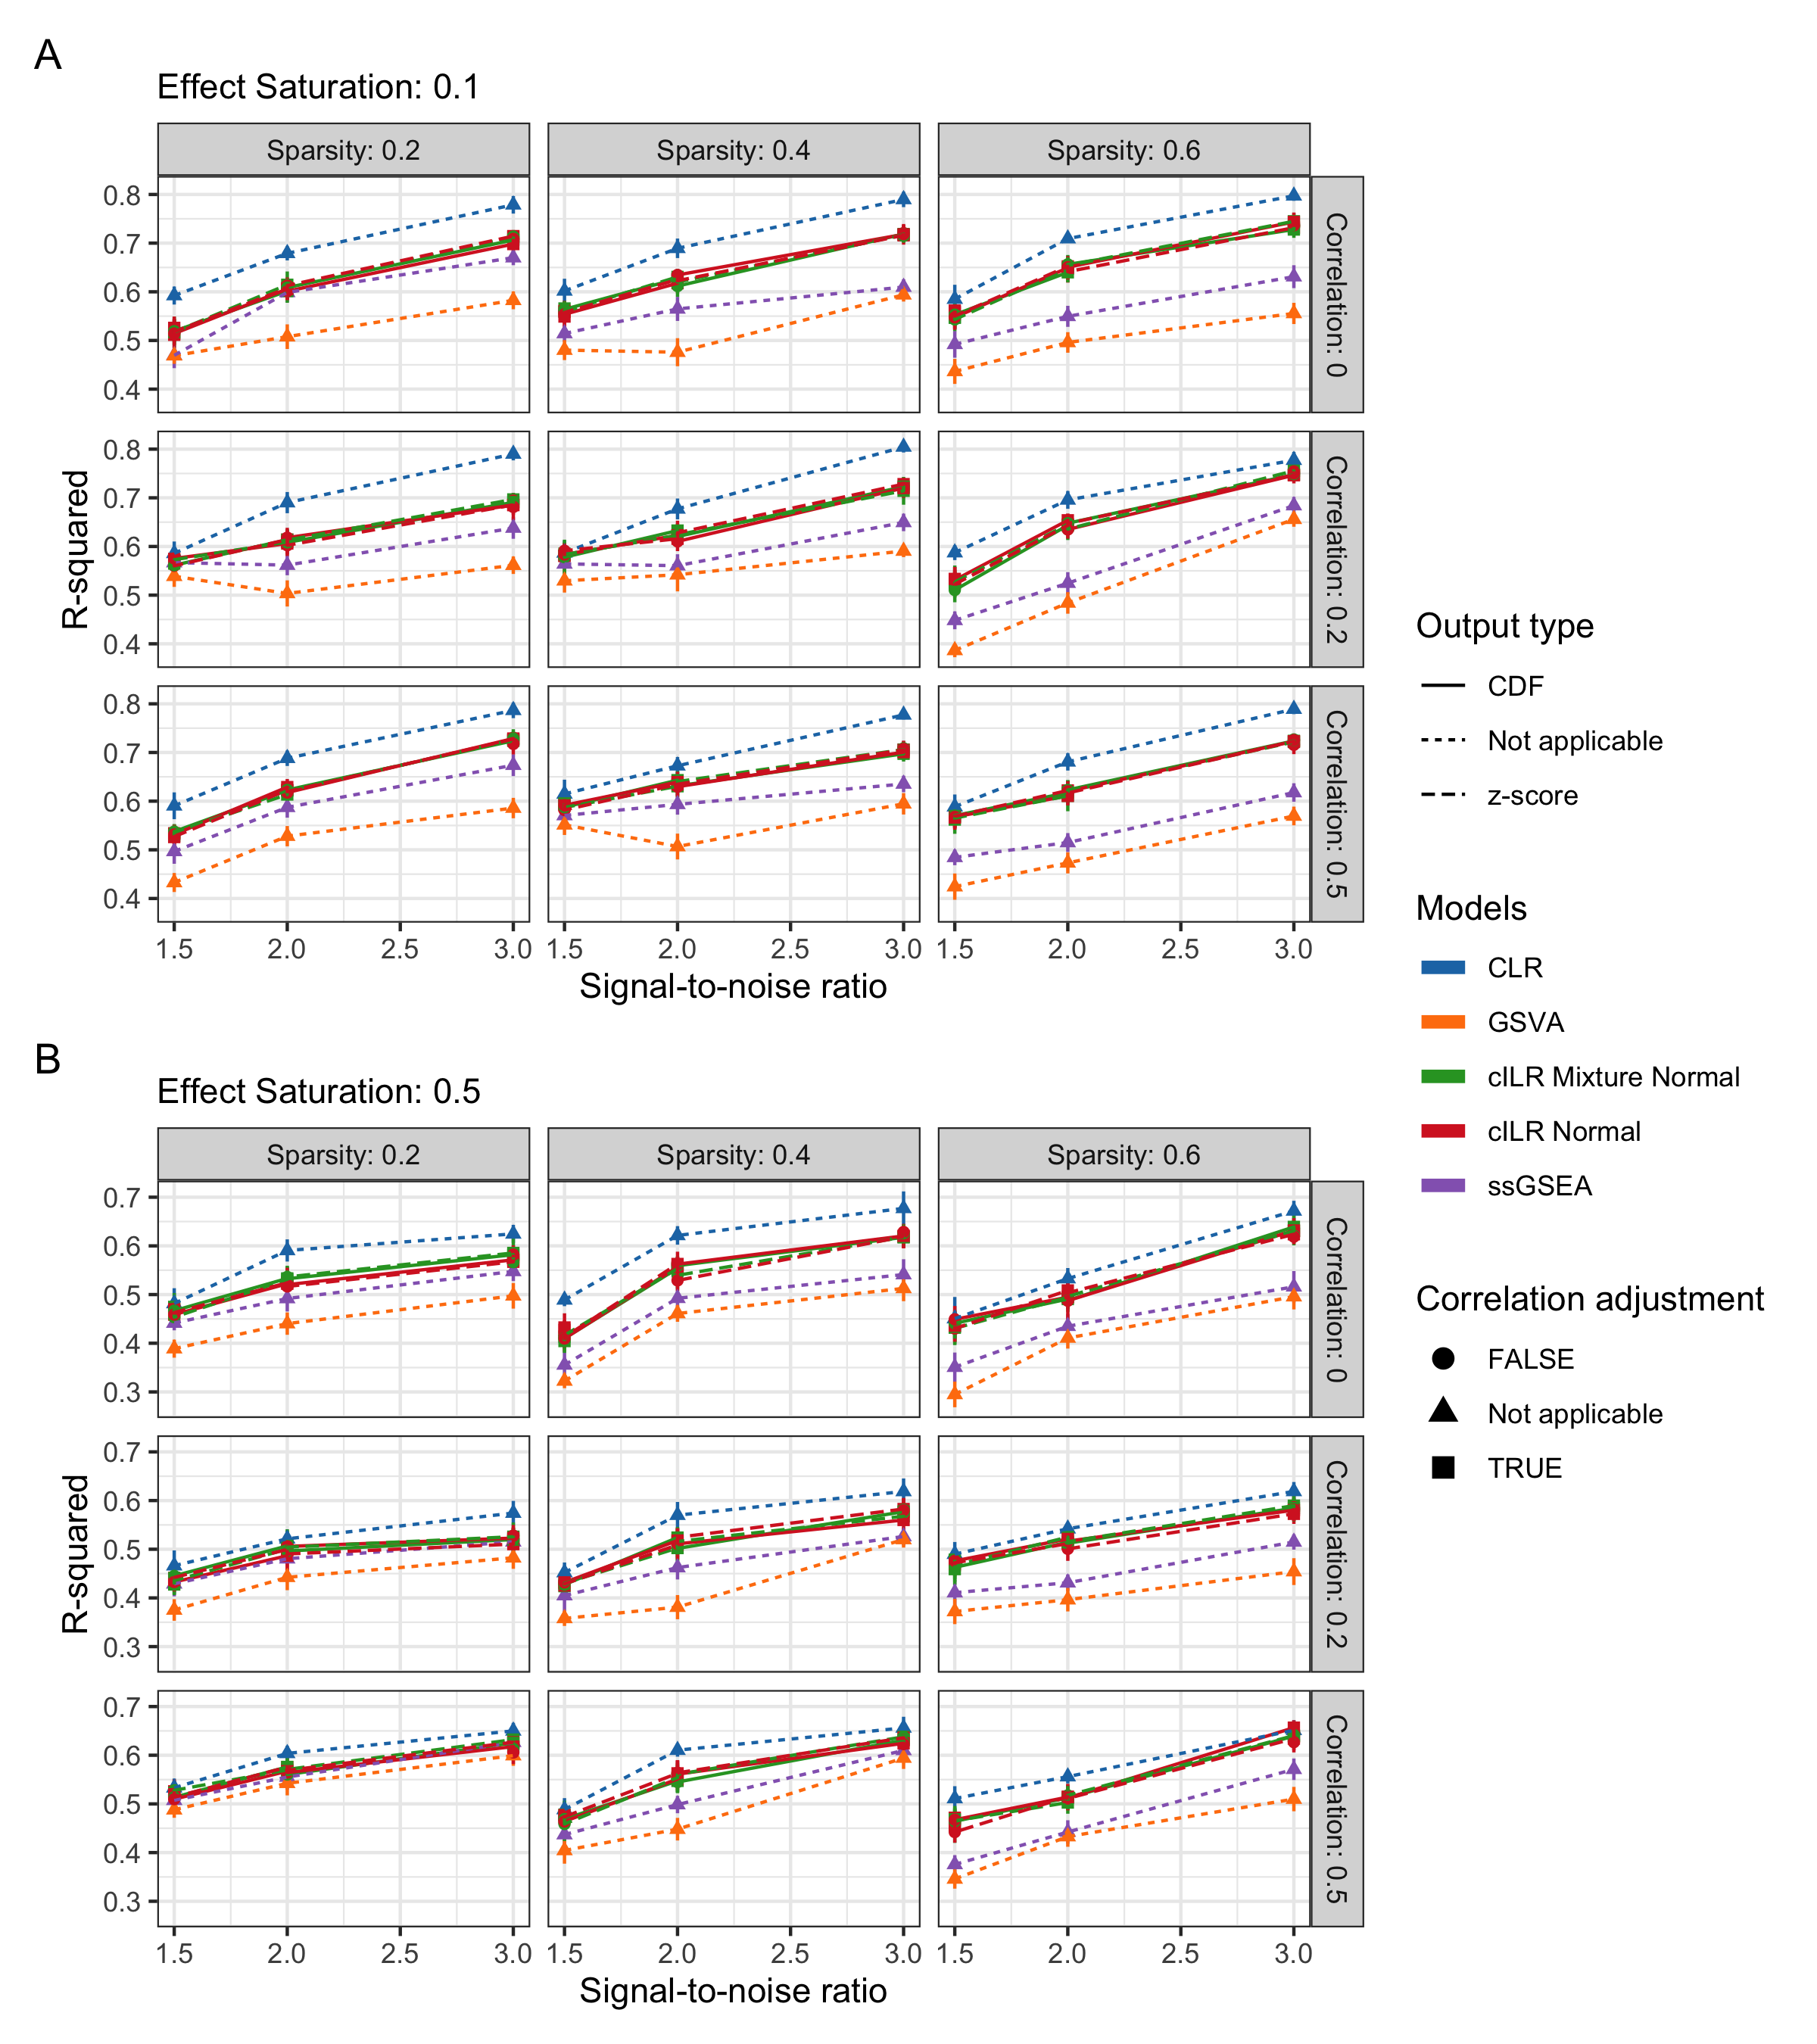
\includegraphics[width=\textwidth]{figures/sim_pred_rsq.png}
%DIF <     \caption{Predictive R-squared of a random forest model for a continuous outcome trained on cILR,     %ssGSEA, GSVA generated scores as well as on standard CLR transformed data evaluated on simulated data %across sparsity levels, correlation, and signal-to-noise ratio. Panel \textbf{(A)} and \textbf{(B)} %represent results across different levels of model saturation (proportion of sets associated with the %outcome). cILR approaches outperformed GSVA and ssGSEA but not standard CLR.}
%DIF >     \caption{Predictive R-squared of a random forest model for a continuous outcome trained on CBEA,     %ssGSEA, GSVA generated scores as well as on standard CLR transformed data evaluated on simulated data %across sparsity levels, correlation, and signal-to-noise ratio. Panel \textbf{(A)} and \textbf{(B)} %represent results across different levels of model saturation (proportion of sets associated with the %outcome). CBEA approaches outperformed GSVA and ssGSEA but not standard CLR.}
%    \label{fig:sim_pred_rsq}
%\end{figure}

\subsubsection*{Real data evaluations}
In addition to parametric simulations, we also assessed the performance of using \DIFdelbegin \DIFdel{cILR }\DIFdelend \DIFaddbegin \DIFadd{CBEA }\DIFaddend scores in predictive models with real data sets. Fig~\ref{fig:7} presents results for two data sets with a similar disease classification task of discriminating patients who are diagnosed with IBD (includes both Crohn's disease and ulcerative colitis) using only microbiome taxonomic composition. The two data sets represent different microbiome sequencing aprpaoches: the Gevers et al. \cite{gevers2014} data set uses 16S rRNA gene sequencing, while the Nielsen et al \cite{nielsen2014} data set uses whole genome shotgun sequencing. 

\begin{figure}[!h]
    \centering
    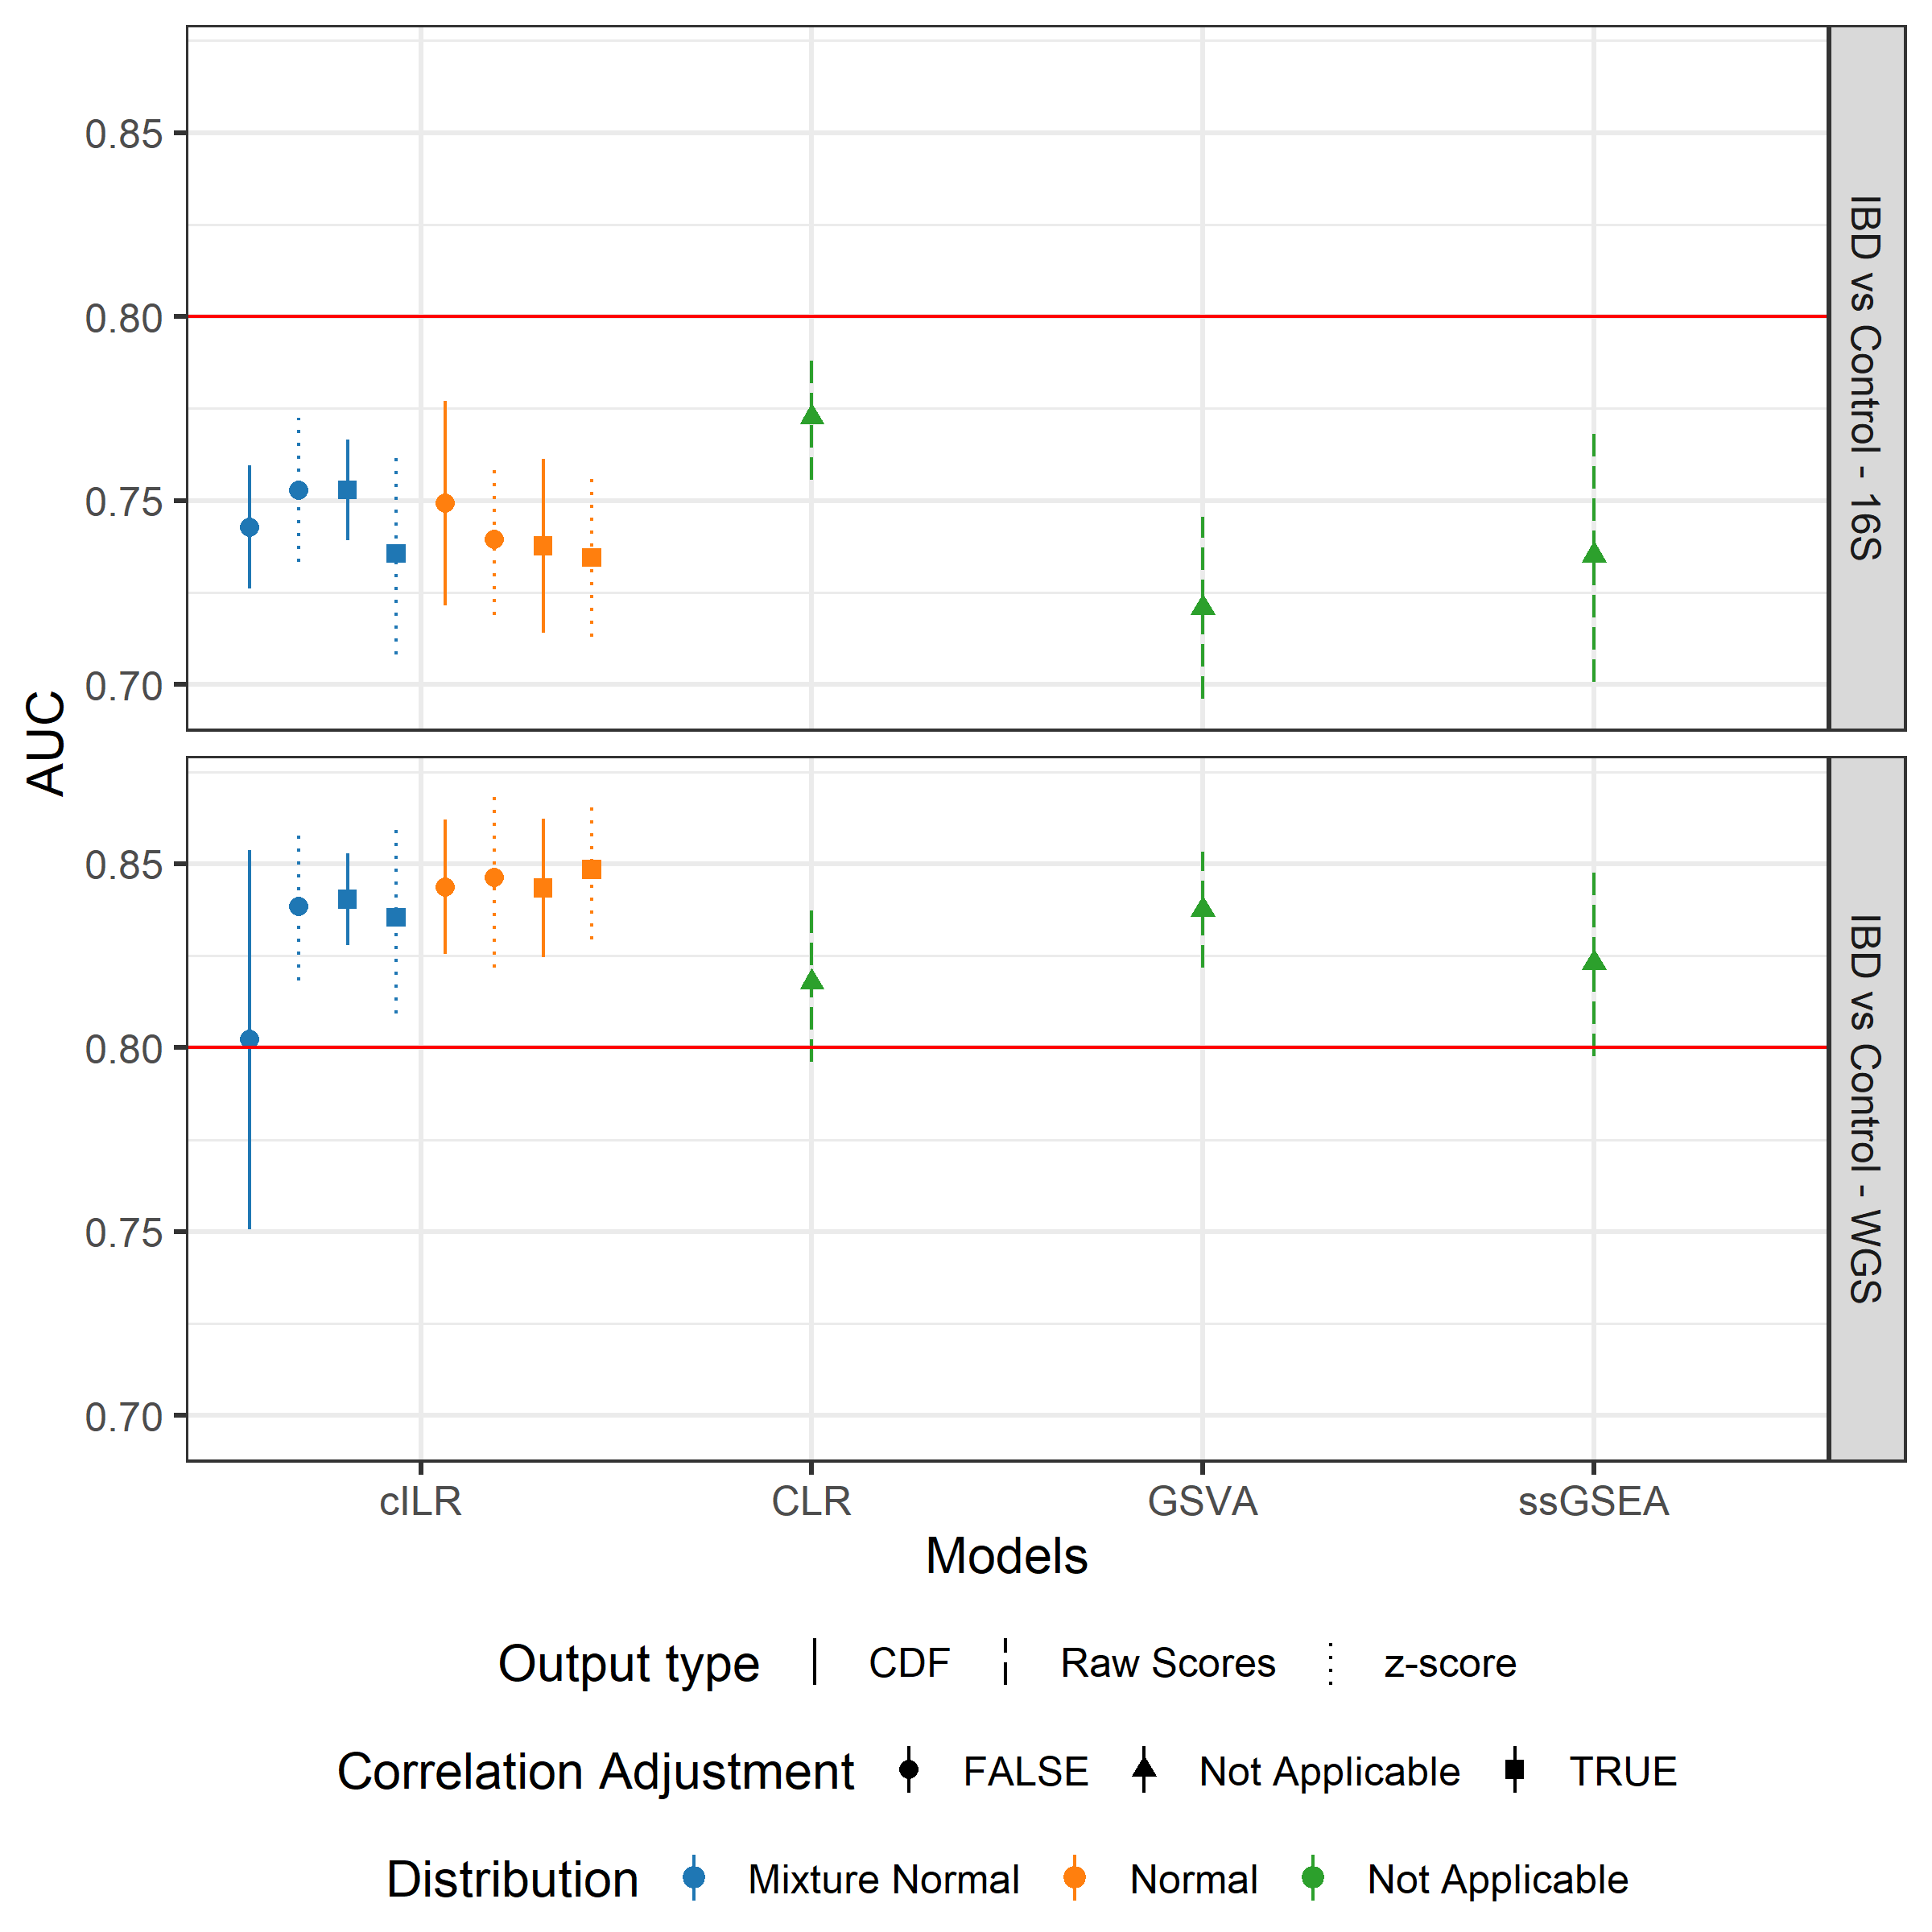
\includegraphics[width = \linewidth]{figures/data_prediction_plot.png}
    \caption{Predictive performance of a naive random forest model trained on \DIFdelbeginFL \DIFdelFL{cILR}\DIFdelendFL \DIFaddbeginFL \DIFaddFL{CBEA}\DIFaddendFL , ssGSEA, GSVA generated scores as well as the standard CLR approach on predicting patients with inflammatory bowel disease versus controls using genus level taxonomic profiles. Data sets used span both 16S rRNA gene sequencing (Gevers et al. \cite{gevers2014}) and whole-genome shotgun sequencing (Nielsen et al. \cite{nielsen2014}). \DIFdelbeginFL \DIFdelFL{cILR }\DIFdelendFL \DIFaddbeginFL \DIFaddFL{CBEA }\DIFaddendFL performs better than GSVA and ssGSEA but not as well as CLR, with the exception of the whole genome sequencing data set.}
    \label{fig:7}
\end{figure}

Similar to simulation experiments, we also fitted a naive random forest model using \DIFdelbegin \DIFdel{CILR}\DIFdelend \DIFaddbegin \DIFadd{CBEA}\DIFaddend , ssGSEA, GSVA, or CLR transformed variables as inputs, and use AUC as the performance criteria. Results also replicated that of the simulations, where across both data sets \DIFdelbegin \DIFdel{cILR }\DIFdelend \DIFaddbegin \DIFadd{CBEA }\DIFaddend and CLR methods provide much better performance than both GSVA or ssGSEA. Interestingly, the \DIFdelbegin \DIFdel{cILR }\DIFdelend \DIFaddbegin \DIFadd{CBEA }\DIFaddend approach performed better than CLR in the whole genome data set but did not perform as well in the 16S rRNA gene sequencing data set. However, these results indicate that \DIFdelbegin \DIFdel{cILR }\DIFdelend \DIFaddbegin \DIFadd{CBEA }\DIFaddend generated scores are informative, providing competitive performance when acting as inputs to disease predictive models. Most importantly, performance values are consistent across both simulated and real data sets. 

These results demonstrate that \DIFdelbegin \DIFdel{cILR }\DIFdelend \DIFaddbegin \DIFadd{CBEA }\DIFaddend generated scores are informative features in disease prediction tasks. Simulation results indicate that \DIFdelbegin \DIFdel{cILR }\DIFdelend \DIFaddbegin \DIFadd{CBEA }\DIFaddend methods perform much better than either GSVA or ssGSEA, but not as well as the standard CLR approach. Interestingly, however, \DIFdelbegin \DIFdel{cILR }\DIFdelend \DIFaddbegin \DIFadd{CBEA }\DIFaddend methods were much more competitive with CLR in either WGS data sets or data sets with higher sparsity levels. 


\section*{Discussion}

\subsection*{Inference with \DIFdelbegin \DIFdel{cILR}\DIFdelend \DIFaddbegin \DIFadd{CBEA}\DIFaddend }
The formulation of \DIFdelbegin \DIFdel{cILR }\DIFdelend \DIFaddbegin \DIFadd{CBEA }\DIFaddend as a comparison between taxa within the set and its complement corresponds to the competitive null hypothesis in the gene set testing literature \cite{tian2005}. This allows for conducting inference with \DIFdelbegin \DIFdel{cILR }\DIFdelend \DIFaddbegin \DIFadd{CBEA }\DIFaddend even at the sample-level. We assessed the usage of \DIFdelbegin \DIFdel{cILR }\DIFdelend \DIFaddbegin \DIFadd{CBEA }\DIFaddend in this type of analysis by evaluating type I error and power across both simulation studies and real data applications. Most importantly, we demonstrated that our adjusted \DIFdelbegin \DIFdel{cILR }\DIFdelend \DIFaddbegin \DIFadd{CBEA }\DIFaddend approach was able to address the issue of variance inflation due to correlation \cite{wu2012} by controlling for type I error at the appropriate $\alpha$ level across different levels of simulated inter-taxa correlation (Fig~\ref{fig:2}) while conversely unadjusted \DIFdelbegin \DIFdel{cILR }\DIFdelend \DIFaddbegin \DIFadd{CBEA }\DIFaddend and the naive Wilcoxon rank sum test showed much higher rates of error. This is further encouraged in real data analysis where the false discovery rate was around $0.05$ when a collection of true null and true alternate hypotheses were tested. Unfortunately the trade-off of good type I error control is lower power. The conservativeness of the test attenuates with higher sparsity and correlation, where power was not approaching even 50\% even at the highest effect sizes. However, when the degree of such data features are reasonable, \DIFdelbegin \DIFdel{cILR }\DIFdelend \DIFaddbegin \DIFadd{CBEA }\DIFaddend will still be able to detect a reasonable proportion of samples with inflated counts.  

We also observed that choosing different distributional forms did not alter performance values for \DIFdelbegin \DIFdel{cILR}\DIFdelend \DIFaddbegin \DIFadd{CBEA}\DIFaddend . This runs contrary to our comparison analysis in Fig~\ref{fig:1}, where we demonstrated that the mixture normal distribution had superior fit compared to the simple normal for raw \DIFdelbegin \DIFdel{cILR }\DIFdelend \DIFaddbegin \DIFadd{CBEA }\DIFaddend scores computed under the global null. We hypothesized that this might be due to the difficulty in fitting mixture distribution to data using the expectation maximization algorithm, as the convergence rate is slow when there is high overlap between the mixtures, resulting in a small mixing coefficient for one of the components \cite{naim2012}. As such, in our implementation of \DIFdelbegin \DIFdel{cILR}\DIFdelend \DIFaddbegin \DIFadd{CBEA}\DIFaddend , in order to ensure convergence for the estimating procedure we increased the number of iterations while relaxing the tolerance parameter. Furthermore, there are also possible problems with our adjustment procedure for the mixture distribution that might impact overall fit. In order to combine the scale and location estimate of two mixture distributions, we fixed the overall mean, standard deviation, mixing coefficient and component-wise means and used an optimization procedure to find the component-wise variances. However, this means that we have one equation for the overall variance but two possible parameters to estimate. As such, there is no guaranteed unique solution to component-wise variances. We hypothesized that the instability and degeneracy in component-wise variance estimates might impact the fidelity of estimates at the tails of the distribution, thereby affecting inference.  

Despite these concerns, empirical results still indicate that \DIFdelbegin \DIFdel{cILR }\DIFdelend \DIFaddbegin \DIFadd{CBEA }\DIFaddend can confidently identify samples with inflated counts. The conservativeness of the correlation adjustment procedure ensures that significant results can be trusted by practitioners, even if \DIFdelbegin \DIFdel{cILR }\DIFdelend \DIFaddbegin \DIFadd{CBEA }\DIFaddend might not be able to exhaustively identify all samples with inflated counts. In situations where either the data is less sparse (e.g. containing a lot of core taxa that are prevalent across all samples), there is less inter-taxa correlation within the set (e.g. taxa that do not participate in common pathways but have shared characteristics like pathogenicity), or if the effect size is large, then \DIFdelbegin \DIFdel{cILR }\DIFdelend \DIFaddbegin \DIFadd{CBEA }\DIFaddend will still be able to produce reasonable power. A practitioner can use \DIFdelbegin \DIFdel{cILR }\DIFdelend \DIFaddbegin \DIFadd{CBEA }\DIFaddend to screen for samples for subsequent analysis that might involve significant costs, or perform hypothesis generation using a less stringent criteria alongside a multiple testing adjustment procedure (such as Benjamini-Hochberg \cite{benjamini1995}). 

\subsection*{Downstream analysis}
The sample-level enrichment scores generated by the \DIFdelbegin \DIFdel{cILR }\DIFdelend \DIFaddbegin \DIFadd{CBEA }\DIFaddend method can be used in downstream analyses commonly performed in microbiome research: differential abundance testing and disease prediction.

\subsubsection*{Differential abundance analysis}
For differential abundance testing, we evaluated whether using \DIFdelbegin \DIFdel{cILR }\DIFdelend \DIFaddbegin \DIFadd{CBEA }\DIFaddend scores alongside a standard difference in means test (Welch's t-test and Wilcoxon rank sum test) is suitable to detect changes in abundance of a set of microbes. We compared \DIFdelbegin \DIFdel{cILR }\DIFdelend \DIFaddbegin \DIFadd{CBEA }\DIFaddend against two popular approaches: corncob \cite{martin2020} and DESeq2 \cite{love2014} applied on data where taxa were aggregated using the naive sum method. We chose DESeq2 because it is an older approach from the bulk RNA-seq literature that has strong support for usage in microbiome taxonomic data \cite{mcmurdie2014}. Conversely, corncob is a newer method developed specifically for microbiome taxonomic data sets, where taxonomic counts are modeled directly using a beta-binomial distribution instead of relying on normalization via size factor estimation like in DESeq2. 

Surprisingly, we found some conflicting results when evaluating comparisons across parametric simulations and real data analysis. The performance of \DIFdelbegin \DIFdel{cILR }\DIFdelend \DIFaddbegin \DIFadd{CBEA }\DIFaddend was consistent across two evaluation criteria, demonstrating good type I error and respectable power. However, corncob and DESeq2 showed opposite effects: in simulation experiments, both methods show good type I error control but low power, while in real data analyses, conversely both corncob and DESeq2 showed inflated type I error but comparable power with respect to \DIFdelbegin \DIFdel{cILR }\DIFdelend \DIFaddbegin \DIFadd{CBEA }\DIFaddend methods. Despite such discrepancy, results still indicate good performance of \DIFdelbegin \DIFdel{cILR }\DIFdelend \DIFaddbegin \DIFadd{CBEA }\DIFaddend scores when used as inputs to downstream differential abundance analysis compared to using aggregated raw counts, even in methods designed to handle that type of data such as corncob and DESeq2.

We hypothesized that the above behavior can arise due to issues with performing inference in the presence taxon-specific protocol biases \cite{mclaren2019}. According to McLaren et al., the observed relative abundance of taxa is different than the true relative abundance due to protocol bias, and importantly this bias is specific to each taxon \cite{mclaren2019}. This is especially true in the context of sum-based aggregations, where the resulting bias of the aggregated taxon are dependent on the relative abundances of the contributing taxa (Appendix I in \cite{mclaren2019}). Conceptually, this means that measurement error for a taxon aggregate is different across samples as relative abundance of contributing changes, leading to issues when attempting to perform inference. As such, we expect methods like corncob or DESeq2 when performed on such aggregates to have inflated type I error compared to our taxon-ratio based approach.  

The bias model also helps explain differences in performance of DESeq2 and corncob in simulation analyses compared to real data. Our simulation protocol does not explicitly include bias in our formulation, and all taxa were generated from the same underlying distribution with similar variances across all samples (the only difference is in the mean value where a taxa is expected to have inflated counts). As such, we do not expect our simulated taxa to have any taxon-specific biases, which is not the case in real data settings. Therefore, we can expect DESeq2 and corncob to retain their expected type I error control in simulation analyses compared to real data. It is still surprising to see lower power for both methods in simulation analyses, which might be due to the fact that the evaluation protocol only considers default settings for both methods and did not attempt to optimize performance. 

The fact that the performance of \DIFdelbegin \DIFdel{cILR }\DIFdelend \DIFaddbegin \DIFadd{CBEA }\DIFaddend remains consistent across both simulation and real data analysis shows that \DIFdelbegin \DIFdel{cILR }\DIFdelend \DIFaddbegin \DIFadd{CBEA }\DIFaddend is invariant to taxon-specific biases. Furthermore, our evaluation indicates that even a simple difference in means test when used in combination with \DIFdelbegin \DIFdel{cILR }\DIFdelend \DIFaddbegin \DIFadd{CBEA }\DIFaddend scores can preserve type I error while maintaining good power. As such, a practioner can use \DIFdelbegin \DIFdel{cILR }\DIFdelend \DIFaddbegin \DIFadd{CBEA }\DIFaddend as a pre-processing step prior to performing a differential abundance test.  

\subsubsection*{Predictive models}
For disease prediction, we fitted a basic random forest model \cite{breiman2001} to predict continuous and binary outcomes using \DIFdelbegin \DIFdel{cILR }\DIFdelend \DIFaddbegin \DIFadd{CBEA }\DIFaddend generated scores as inputs. Similar to our inference analysis, we compared \DIFdelbegin \DIFdel{cILR }\DIFdelend \DIFaddbegin \DIFadd{CBEA }\DIFaddend against both ssGSEA and GSVA. Additionally, we also evaluated \DIFdelbegin \DIFdel{cILR }\DIFdelend \DIFaddbegin \DIFadd{CBEA }\DIFaddend with the approach where counts of a set were aggregated using sums and then centered log-ratio transformed. This is because CLR is considered standard practice in using microbiome variables as predictors for a model \cite{gloor2017}. Results indicated that \DIFdelbegin \DIFdel{cILR }\DIFdelend \DIFaddbegin \DIFadd{CBEA }\DIFaddend produces good performance values across both real data analysis and simulation scenarios. Since predictive models consider the effect of variables jointly (and in the case of random forest, consider interactions as well), good performance indicates that \DIFdelbegin \DIFdel{cILR }\DIFdelend \DIFaddbegin \DIFadd{CBEA }\DIFaddend scores can capture joint distribution of sets, enabling both uniset and multi-set type analyses. Comparatively, \DIFdelbegin \DIFdel{cILR }\DIFdelend \DIFaddbegin \DIFadd{CBEA }\DIFaddend generated scores outperformed other enrichment score methods (GSVA and ssGSEA), suggesting that it is more tailored for microbiome taxonomic data sets. This is consistent with our sample ranking analysis (Fig~\ref{fig:3}), where \DIFdelbegin \DIFdel{cILR }\DIFdelend \DIFaddbegin \DIFadd{CBEA }\DIFaddend scores are on average more informative when used to rank samples based on their propensity to have inflated counts. However, \DIFdelbegin \DIFdel{cILR }\DIFdelend \DIFaddbegin \DIFadd{CBEA }\DIFaddend did not outperform the CLR approach across our simulation studies, and only marginally performed better in the real data analysis with WGS data. 

However, in simulation studies, this performance gap between CLR and \DIFdelbegin \DIFdel{cILR }\DIFdelend \DIFaddbegin \DIFadd{CBEA }\DIFaddend decreases with higher sparsity and correlation, especially in low effect saturation scenarios. Additionally, there are also downsides to applying CLR. First, the singular covariance matrix of CLR transformed variables is singular due to a sum to zero constraint \cite{gloor2017}, preventing the proper usage of approaches that rely on matrix decomposition. Second, the procedure still relies on using summation of counts prior to transformation, which means that we still can't compare across sets of different sizes, and any bias might still be propagated \cite{mclaren2019}. As such, despite benefits in performance for a naive random forest model, there is still space for using \DIFdelbegin \DIFdel{cILR }\DIFdelend \DIFaddbegin \DIFadd{CBEA }\DIFaddend as primary inputs into predictive models. 

Similar to other experiments in downstream usage of \DIFdelbegin \DIFdel{cILR}\DIFdelend \DIFaddbegin \DIFadd{CBEA}\DIFaddend , performance did not change with different underlying distributions, output types, or correlation status. This is surprising since we expect z-scores to perform better as they are able to capture the direction of an association. The fact that this effect persisted even onto our real data analysis suggests that this is not due to a deficiency of our simulation design. As such, practitioners who wish to use \DIFdelbegin \DIFdel{cILR }\DIFdelend \DIFaddbegin \DIFadd{CBEA }\DIFaddend in predictive models might be suited to use the settings that is the fastest to compute.  

Ultimately, results indicate that \DIFdelbegin \DIFdel{cILR }\DIFdelend \DIFaddbegin \DIFadd{CBEA }\DIFaddend can produce informative scores that contribute to competitive performance of prediction models even in low signal-to-noise ratios with high inter-taxa correlation and sparsity. Even though there exists situations where it might not provide maximum predictive values, the flexibility of \DIFdelbegin \DIFdel{cILR }\DIFdelend \DIFaddbegin \DIFadd{CBEA }\DIFaddend in various types of analyses enable even though in some scenarios it might not provide maximum predictive values. 

\subsection*{Limitations and future directions} 
There are various limitations to our evaluation of \DIFdelbegin \DIFdel{cILR}\DIFdelend \DIFaddbegin \DIFadd{CBEA}\DIFaddend . First, our simulation analysis might not capture the appropriate data-generating distributions underlying microbiome taxonomic data. There is strong evidence to suggest that our zero-inflated negative binomial distribution is representative \cite{calgaro2020}, however other distributions such as the Dirichlet multinomial distribution \cite{wu2016} have been used in the evaluation of prior studies. Second, the usage of the gingival data set similar to \cite{calgaro2020} to assess power in differential abundance testing and single sample inference is not perfect. This is because the oxygen usage label of each microbe in the data set is only available at the genus level, and the difference in counts for obligate aerobes and anaerobes across the supragingival and subgingival sites might not be as clear cut. As such, results from power analyses using this data set is only relative between the comparison methods. Finally, we assumed that taxa within a set are all equally associated with the outcome. This limits our ability to evaluate the performance of \DIFdelbegin \DIFdel{cILR }\DIFdelend \DIFaddbegin \DIFadd{CBEA }\DIFaddend when only a small number of taxa within the set is associated with the outcome, or if there are variability in effect sizes or association direction of taxa within a set. 

Our evaluation showed various drawbacks of the \DIFdelbegin \DIFdel{cILR }\DIFdelend \DIFaddbegin \DIFadd{CBEA }\DIFaddend method. First, inference with \DIFdelbegin \DIFdel{cILR }\DIFdelend \DIFaddbegin \DIFadd{CBEA }\DIFaddend is limited in being able to exhaustively detect all samples with significant inflated counts for a set in situations where there is a high degree of sparsity and inter-taxa correlation. Second, for downstream analyses, \DIFdelbegin \DIFdel{cILR }\DIFdelend \DIFaddbegin \DIFadd{CBEA }\DIFaddend might not always perform better than competing methods, especially when being used to generate inputs to predictive models. We hypothesized that this might be due to the lack of fit for the underlying null distribution in high correlation settings, especially the identifiability problem associated with adjusting the mixture normal distribution. As such, we hope to refine the null distribution estimating procedure by either choosing a better distributional form, or to further constrain the optimization procedure of the mixture normal distribution by fixing the third and fourth moments. 

In addition, there are possible extensions \DIFdelbegin \DIFdel{cILR }\DIFdelend \DIFaddbegin \DIFadd{CBEA }\DIFaddend can we can consider to provide more flexibility across different data analysis scenarios in data analysis. First, \DIFdelbegin \DIFdel{cILR }\DIFdelend \DIFaddbegin \DIFadd{CBEA }\DIFaddend did not address the sparsity of microbiome taxonomic data and relies on a pseudocount to ensure log operations are valid. We can address this by incorporating more sophisticated model-based zero-correction methods such as in \cite{martin-fernandez2012} or \cite{kaul2017a}. Second, \DIFdelbegin \DIFdel{cILR }\DIFdelend \DIFaddbegin \DIFadd{CBEA }\DIFaddend also treated all taxa within the set as equally contributing to the set. Incorporation of taxa-specific weights could reduce the influence of outliers, such as rare or highly invariant taxa. Finally, curating sets based on \emph{apriori} characteristics of microbes can allow for incorporating functional insights into microbiome-outcome analyses while also improving interpretability when compared to using taxonomic categories such as phylum or genus alone.  

\section*{Conclusion}
Gene set testing, or pathway analysis is an important tool in the analysis of high-dimensional genomics data sets. However, limited work has been done developing set based methods specifically for microbiome relative abundance data. We introduced a new microbiome-specific method to generate set-based enrichment scores at the sample level. We demonstrated that our method can control for type I error for significance testing at the sample level, while generated scores are also valid inputs in downstream analyses, including disease prediction and differential abundance.  

\section*{Acknowledgments}
The authors thank Becky Lebeaux, Modupe Coker, Erika Dade, Jie Zhou, and Weston Viles for insightful comments and suggestions that greatly improved the paper. 

\nolinenumbers
% Either type in your references using
% \begin{thebibliography}{}
% \bibitem{}
% Text
% \end{thebibliography}
%
% or
%
% Compile your BiBTeX database using our plos2015.bst
% style file and paste the contents of your .bbl file
% here. See http://journals.plos.org/plosone/s/latex for 
% step-by-step instructions.
% 

%DIF <  \bibliography{tax_agg}{}
\DIFaddbegin \bibliography{mac_taxagg}{}
\DIFaddend 



\DIFdelbegin %DIFDELCMD < \begin{thebibliography}{10}
%DIFDELCMD < 

%DIFDELCMD < \bibitem{proctor2019}
\DIFdel{Proctor LM, Creasy HH, Fettweis JM, }%DIFDELCMD < {%%%
\DIFdel{Lloyd-Price}%DIFDELCMD < } %%%
\DIFdel{J, Mahurkar A, Zhou W, et~al.
}%DIFDELCMD < \newblock %%%
\DIFdel{The }%DIFDELCMD < {{%%%
\DIFdel{Integrative Human Microbiome Project}%DIFDELCMD < }}%%%
\DIFdel{.
}%DIFDELCMD < \newblock %%%
\DIFdel{Nature. 2019;569(7758):641--648.
}%DIFDELCMD < \newblock %%%
\DIFdel{doi:}%DIFDELCMD < {%%%
\DIFdel{10.1038/s41586-019-1238-8}%DIFDELCMD < }%%%
\DIFdel{.
}%DIFDELCMD < 

%DIFDELCMD < \bibitem{sharma2019}
\DIFdel{Sharma S, Tripathi P.
}%DIFDELCMD < \newblock %%%
\DIFdel{Gut Microbiome and Type 2 Diabetes: Where We Are and Where to Go?
}%DIFDELCMD < \newblock %%%
\DIFdel{The Journal of Nutritional Biochemistry. 2019;63:101--108.
}%DIFDELCMD < \newblock %%%
\DIFdel{doi:}%DIFDELCMD < {%%%
\DIFdel{10.1016/j.jnutbio.2018.10.003}%DIFDELCMD < }%%%
\DIFdel{.
}%DIFDELCMD < 

%DIFDELCMD < \bibitem{aoun2020}
\DIFdel{Aoun A, Darwish F, Hamod N.
}%DIFDELCMD < \newblock %%%
\DIFdel{The }%DIFDELCMD < {{%%%
\DIFdel{Influence}%DIFDELCMD < }} %%%
\DIFdel{of the }%DIFDELCMD < {{%%%
\DIFdel{Gut Microbiome}%DIFDELCMD < }} %%%
\DIFdel{on }%DIFDELCMD < {{%%%
\DIFdel{Obesity}%DIFDELCMD < }} %%%
\DIFdel{in
  }%DIFDELCMD < {{%%%
\DIFdel{Adults}%DIFDELCMD < }} %%%
\DIFdel{and the }%DIFDELCMD < {{%%%
\DIFdel{Role}%DIFDELCMD < }} %%%
\DIFdel{of }%DIFDELCMD < {{%%%
\DIFdel{Probiotics}%DIFDELCMD < }}%%%
\DIFdel{, }%DIFDELCMD < {{%%%
\DIFdel{Prebiotics}%DIFDELCMD < }}%%%
\DIFdel{, and
  }%DIFDELCMD < {{%%%
\DIFdel{Synbiotics}%DIFDELCMD < }} %%%
\DIFdel{for }%DIFDELCMD < {{%%%
\DIFdel{Weight Loss}%DIFDELCMD < }}%%%
\DIFdel{.
}%DIFDELCMD < \newblock %%%
\DIFdel{Preventive Nutrition and Food Science. 2020;25(2):113--123.
}%DIFDELCMD < \newblock %%%
\DIFdel{doi:}%DIFDELCMD < {%%%
\DIFdel{10.3746/pnf.2020.25.2.113}%DIFDELCMD < }%%%
\DIFdel{.
}%DIFDELCMD < 

%DIFDELCMD < \bibitem{cho2012}
\DIFdel{Cho I, Blaser MJ.
}%DIFDELCMD < \newblock %%%
\DIFdel{The Human Microbiome: At the Interface of Health and Disease.
}%DIFDELCMD < \newblock %%%
\DIFdel{Nature Reviews Genetics. 2012;13(4):260--270.
}%DIFDELCMD < \newblock %%%
\DIFdel{doi:}%DIFDELCMD < {%%%
\DIFdel{10.1038/nrg3182}%DIFDELCMD < }%%%
\DIFdel{.
}%DIFDELCMD < 

%DIFDELCMD < \bibitem{callahan2016}
\DIFdel{Callahan BJ, McMurdie PJ, Rosen MJ, Han AW, Johnson AJA, Holmes SP.
}%DIFDELCMD < \newblock {{DADA2}}%%%
\DIFdel{: }%DIFDELCMD < {{%%%
\DIFdel{High}%DIFDELCMD < }}%%%
\DIFdel{-Resolution Sample Inference from }%DIFDELCMD < {{%%%
\DIFdel{Illumina}%DIFDELCMD < }}
%DIFDELCMD <   %%%
\DIFdel{Amplicon Data.
}%DIFDELCMD < \newblock %%%
\DIFdel{Nature Methods. 2016;13(7):581--583.
}%DIFDELCMD < \newblock %%%
\DIFdel{doi:}%DIFDELCMD < {%%%
\DIFdel{10.1038/nmeth.3869}%DIFDELCMD < }%%%
\DIFdel{.
}%DIFDELCMD < 

%DIFDELCMD < \bibitem{truong2015}
\DIFdel{Truong DT, Franzosa EA, Tickle TL, Scholz M, Weingart G, Pasolli E, et~al.
}%DIFDELCMD < \newblock {{MetaPhlAn2}} %%%
\DIFdel{for Enhanced Metagenomic Taxonomic Profiling.
}%DIFDELCMD < \newblock %%%
\DIFdel{Nature Methods. 2015;12(10):902--903.
}%DIFDELCMD < \newblock %%%
\DIFdel{doi:}%DIFDELCMD < {%%%
\DIFdel{10.1038/nmeth.3589}%DIFDELCMD < }%%%
\DIFdel{.
}%DIFDELCMD < 

%DIFDELCMD < \bibitem{li2019}
\DIFdel{Li H.
}%DIFDELCMD < \newblock %%%
\DIFdel{Statistical and }%DIFDELCMD < {{%%%
\DIFdel{Computational Methods}%DIFDELCMD < }} %%%
\DIFdel{in }%DIFDELCMD < {{%%%
\DIFdel{Microbiome}%DIFDELCMD < }} %%%
\DIFdel{and
  }%DIFDELCMD < {{%%%
\DIFdel{Metagenomics}%DIFDELCMD < }}%%%
\DIFdel{.
}%DIFDELCMD < \newblock %%%
\DIFdel{In: Handbook of }%DIFDELCMD < {{%%%
\DIFdel{Statistical Genomics}%DIFDELCMD < }}%%%
\DIFdel{. }%DIFDELCMD < {%%%
\DIFdel{John Wiley \& Sons, Ltd}%DIFDELCMD < }%%%
\DIFdel{;
  2019. p. 977--550.
}%DIFDELCMD < 

%DIFDELCMD < \bibitem{li2015}
\DIFdel{Li H.
}%DIFDELCMD < \newblock %%%
\DIFdel{Microbiome, }%DIFDELCMD < {{%%%
\DIFdel{Metagenomics}%DIFDELCMD < }}%%%
\DIFdel{, and }%DIFDELCMD < {{%%%
\DIFdel{High}%DIFDELCMD < }}%%%
\DIFdel{-}%DIFDELCMD < {{%%%
\DIFdel{Dimensional
  Compositional Data Analysis}%DIFDELCMD < }}%%%
\DIFdel{.
}%DIFDELCMD < \newblock %%%
\DIFdel{Annual Review of Statistics and Its Application. 2015;2(1):73--94.
}%DIFDELCMD < \newblock %%%
\DIFdel{doi:}%DIFDELCMD < {%%%
\DIFdel{10.1146/annurev-statistics-010814-020351}%DIFDELCMD < }%%%
\DIFdel{.
}%DIFDELCMD < 

%DIFDELCMD < \bibitem{shi2016}
\DIFdel{Shi P, Zhang A, Li H.
}%DIFDELCMD < \newblock %%%
\DIFdel{Regression Analysis for Microbiome Compositional Data.
}%DIFDELCMD < \newblock %%%
\DIFdel{The Annals of Applied Statistics. 2016;10(2):1019--1040.
}%DIFDELCMD < \newblock %%%
\DIFdel{doi:}%DIFDELCMD < {%%%
\DIFdel{10.1214/16-AOAS928}%DIFDELCMD < }%%%
\DIFdel{.
}%DIFDELCMD < 

%DIFDELCMD < \bibitem{sankaran2014}
\DIFdel{Sankaran K, Holmes S.
}%DIFDELCMD < \newblock {{structSSI}}%%%
\DIFdel{: }%DIFDELCMD < {{%%%
\DIFdel{Simultaneous}%DIFDELCMD < }} %%%
\DIFdel{and }%DIFDELCMD < {{%%%
\DIFdel{Selective Inference}%DIFDELCMD < }} %%%
\DIFdel{for
  }%DIFDELCMD < {{%%%
\DIFdel{Grouped}%DIFDELCMD < }} %%%
\DIFdel{or }%DIFDELCMD < {{%%%
\DIFdel{Hierarchically Structured Data}%DIFDELCMD < }}%%%
\DIFdel{.
}%DIFDELCMD < \newblock %%%
\DIFdel{Journal of statistical software. 2014;59(13):1--21.
}%DIFDELCMD < \newblock %%%
\DIFdel{doi:}%DIFDELCMD < {%%%
\DIFdel{10.18637/jss.v059.i13}%DIFDELCMD < }%%%
\DIFdel{.
}%DIFDELCMD < 

%DIFDELCMD < \bibitem{benjamini1995}
\DIFdel{Benjamini Y, Hochberg Y.
}%DIFDELCMD < \newblock %%%
\DIFdel{Controlling the }%DIFDELCMD < {{%%%
\DIFdel{False Discovery Rate}%DIFDELCMD < }}%%%
\DIFdel{: }%DIFDELCMD < {{%%%
\DIFdel{A Practical}%DIFDELCMD < }} %%%
\DIFdel{and
  }%DIFDELCMD < {{%%%
\DIFdel{Powerful Approach}%DIFDELCMD < }} %%%
\DIFdel{to }%DIFDELCMD < {{%%%
\DIFdel{Multiple Testing}%DIFDELCMD < }}%%%
\DIFdel{.
}%DIFDELCMD < \newblock %%%
\DIFdel{Journal of the Royal Statistical Society Series B (Methodological).
  1995;57(1):289--300.
}%DIFDELCMD < 

%DIFDELCMD < \bibitem{chen2018}
\DIFdel{Chen J, King E, Deek R, Wei Z, Yu Y, Grill D, et~al.
}%DIFDELCMD < \newblock %%%
\DIFdel{An Omnibus Test for Differential Distribution Analysis of Microbiome
  Sequencing Data.
}%DIFDELCMD < \newblock %%%
\DIFdel{Bioinformatics. 2018;34(4):643--651.
}%DIFDELCMD < \newblock %%%
\DIFdel{doi:}%DIFDELCMD < {%%%
\DIFdel{10.1093/bioinformatics/btx650}%DIFDELCMD < }%%%
\DIFdel{.
}%DIFDELCMD < 

%DIFDELCMD < \bibitem{weiss2017}
\DIFdel{Weiss S, Xu ZZ, Peddada S, Amir A, Bittinger K, Gonzalez A, et~al.
}%DIFDELCMD < \newblock %%%
\DIFdel{Normalization and Microbial Differential Abundance Strategies Depend
  upon Data Characteristics.
}%DIFDELCMD < \newblock %%%
\DIFdel{Microbiome. 2017;5(1).
}%DIFDELCMD < \newblock %%%
\DIFdel{doi:}%DIFDELCMD < {%%%
\DIFdel{10.1186/s40168-017-0237-y}%DIFDELCMD < }%%%
\DIFdel{.
}%DIFDELCMD < 

%DIFDELCMD < \bibitem{mcmurdie2014}
\DIFdel{McMurdie PJ, Holmes S.
}%DIFDELCMD < \newblock %%%
\DIFdel{Waste }%DIFDELCMD < {{%%%
\DIFdel{Not}%DIFDELCMD < }}%%%
\DIFdel{, }%DIFDELCMD < {{%%%
\DIFdel{Want Not}%DIFDELCMD < }}%%%
\DIFdel{: }%DIFDELCMD < {{%%%
\DIFdel{Why Rarefying Microbiome Data Is
  Inadmissible}%DIFDELCMD < }}%%%
\DIFdel{.
}%DIFDELCMD < \newblock %%%
\DIFdel{PLOS Computational Biology. 2014;10(4):e1003531.
}%DIFDELCMD < \newblock %%%
\DIFdel{doi:}%DIFDELCMD < {%%%
\DIFdel{10.1371/journal.pcbi.1003531}%DIFDELCMD < }%%%
\DIFdel{.
}%DIFDELCMD < 

%DIFDELCMD < \bibitem{love2014}
\DIFdel{Love MI, Huber W, Anders S.
}%DIFDELCMD < \newblock %%%
\DIFdel{Moderated Estimation of Fold Change and Dispersion for }%DIFDELCMD < {{%%%
\DIFdel{RNA}%DIFDELCMD < }}%%%
\DIFdel{-Seq
  Data with }%DIFDELCMD < {{%%%
\DIFdel{DESeq2}%DIFDELCMD < }}%%%
\DIFdel{.
}%DIFDELCMD < \newblock %%%
\DIFdel{Genome Biology. 2014;15(12):550.
}%DIFDELCMD < \newblock %%%
\DIFdel{doi:}%DIFDELCMD < {%%%
\DIFdel{10.1186/s13059-014-0550-8}%DIFDELCMD < }%%%
\DIFdel{.
}%DIFDELCMD < 

%DIFDELCMD < \bibitem{quinn2019}
\DIFdel{Quinn TP, Erb I, Gloor G, Notredame C, Richardson MF, Crowley TM.
}%DIFDELCMD < \newblock %%%
\DIFdel{A Field Guide for the Compositional Analysis of Any-Omics Data.
}%DIFDELCMD < \newblock %%%
\DIFdel{GigaScience. 2019;8(giz107).
}%DIFDELCMD < \newblock %%%
\DIFdel{doi:}%DIFDELCMD < {%%%
\DIFdel{10.1093/gigascience/giz107}%DIFDELCMD < }%%%
\DIFdel{.
}%DIFDELCMD < 

%DIFDELCMD < \bibitem{quinn2018b}
\DIFdel{Quinn TP, Erb I, Richardson MF, Crowley TM.
}%DIFDELCMD < \newblock %%%
\DIFdel{Understanding Sequencing Data as Compositions: An Outlook and Review.
}%DIFDELCMD < \newblock %%%
\DIFdel{Bioinformatics. 2018;34(16):2870--2878.
}%DIFDELCMD < \newblock %%%
\DIFdel{doi:}%DIFDELCMD < {%%%
\DIFdel{10.1093/bioinformatics/bty175}%DIFDELCMD < }%%%
\DIFdel{.
}%DIFDELCMD < 

%DIFDELCMD < \bibitem{gloor2017}
\DIFdel{Gloor GB, Macklaim JM, }%DIFDELCMD < {%%%
\DIFdel{Pawlowsky-Glahn}%DIFDELCMD < } %%%
\DIFdel{V, Egozcue JJ.
}%DIFDELCMD < \newblock %%%
\DIFdel{Microbiome }%DIFDELCMD < {{%%%
\DIFdel{Datasets Are Compositional}%DIFDELCMD < }}%%%
\DIFdel{: }%DIFDELCMD < {{%%%
\DIFdel{And This Is Not
  Optional}%DIFDELCMD < }}%%%
\DIFdel{.
}%DIFDELCMD < \newblock %%%
\DIFdel{Frontiers in Microbiology. 2017;8.
}%DIFDELCMD < \newblock %%%
\DIFdel{doi:}%DIFDELCMD < {%%%
\DIFdel{10.3389/fmicb.2017.02224}%DIFDELCMD < }%%%
\DIFdel{.
}%DIFDELCMD < 

%DIFDELCMD < \bibitem{aitchison1999}
\DIFdel{Aitchison J.
}%DIFDELCMD < \newblock %%%
\DIFdel{A }%DIFDELCMD < {{%%%
\DIFdel{Concise Guide}%DIFDELCMD < }} %%%
\DIFdel{to }%DIFDELCMD < {{%%%
\DIFdel{Compositional Data Analysis}%DIFDELCMD < }}%%%
\DIFdel{. 1999; p. 134.
}%DIFDELCMD < 

%DIFDELCMD < \bibitem{kurtz2015}
\DIFdel{Kurtz ZD, M}%DIFDELCMD < {%%%
\DIFdel{\"u}%DIFDELCMD < }%%%
\DIFdel{ller CL, Miraldi ER, Littman DR, Blaser MJ, Bonneau RA.
}%DIFDELCMD < \newblock %%%
\DIFdel{Sparse and }%DIFDELCMD < {{%%%
\DIFdel{Compositionally Robust Inference}%DIFDELCMD < }} %%%
\DIFdel{of }%DIFDELCMD < {{%%%
\DIFdel{Microbial
  Ecological Networks}%DIFDELCMD < }}%%%
\DIFdel{.
}%DIFDELCMD < \newblock %%%
\DIFdel{PLOS Computational Biology. 2015;11(5):e1004226.
}%DIFDELCMD < \newblock %%%
\DIFdel{doi:}%DIFDELCMD < {%%%
\DIFdel{10.1371/journal.pcbi.1004226}%DIFDELCMD < }%%%
\DIFdel{.
}%DIFDELCMD < 

%DIFDELCMD < \bibitem{kaul2017}
\DIFdel{Kaul A, Davidov O, Peddada SD.
}%DIFDELCMD < \newblock %%%
\DIFdel{Structural Zeros in High-Dimensional Data with Applications to
  Microbiome Studies.
}%DIFDELCMD < \newblock %%%
\DIFdel{Biostatistics. 2017;18(3):422--433.
}%DIFDELCMD < \newblock %%%
\DIFdel{doi:}%DIFDELCMD < {%%%
\DIFdel{10.1093/biostatistics/kxw053}%DIFDELCMD < }%%%
\DIFdel{.
}%DIFDELCMD < 

%DIFDELCMD < \bibitem{kaul2017a}
\DIFdel{Kaul A, Mandal S, Davidov O, Peddada SD.
}%DIFDELCMD < \newblock %%%
\DIFdel{Analysis of }%DIFDELCMD < {{%%%
\DIFdel{Microbiome Data}%DIFDELCMD < }} %%%
\DIFdel{in the }%DIFDELCMD < {{%%%
\DIFdel{Presence}%DIFDELCMD < }} %%%
\DIFdel{of }%DIFDELCMD < {{%%%
\DIFdel{Excess
  Zeros}%DIFDELCMD < }}%%%
\DIFdel{.
}%DIFDELCMD < \newblock %%%
\DIFdel{Frontiers in Microbiology. 2017;8.
}%DIFDELCMD < \newblock %%%
\DIFdel{doi:}%DIFDELCMD < {%%%
\DIFdel{10.3389/fmicb.2017.02114}%DIFDELCMD < }%%%
\DIFdel{.
}%DIFDELCMD < 

%DIFDELCMD < \bibitem{khatri2012}
\DIFdel{Khatri P, Sirota M, Butte AJ.
}%DIFDELCMD < \newblock %%%
\DIFdel{Ten }%DIFDELCMD < {{%%%
\DIFdel{Years}%DIFDELCMD < }} %%%
\DIFdel{of }%DIFDELCMD < {{%%%
\DIFdel{Pathway Analysis}%DIFDELCMD < }}%%%
\DIFdel{: }%DIFDELCMD < {{%%%
\DIFdel{Current Approaches}%DIFDELCMD < }} %%%
\DIFdel{and
  }%DIFDELCMD < {{%%%
\DIFdel{Outstanding Challenges}%DIFDELCMD < }}%%%
\DIFdel{.
}%DIFDELCMD < \newblock %%%
\DIFdel{PLOS Computational Biology. 2012;8(2):e1002375.
}%DIFDELCMD < \newblock %%%
\DIFdel{doi:}%DIFDELCMD < {%%%
\DIFdel{10.1371/journal.pcbi.1002375}%DIFDELCMD < }%%%
\DIFdel{.
}%DIFDELCMD < 

%DIFDELCMD < \bibitem{goeman2007}
\DIFdel{Goeman JJ, B}%DIFDELCMD < {%%%
\DIFdel{\"u}%DIFDELCMD < }%%%
\DIFdel{hlmann P.
}%DIFDELCMD < \newblock %%%
\DIFdel{Analyzing Gene Expression Data in Terms of Gene Sets: Methodological
  Issues.
}%DIFDELCMD < \newblock %%%
\DIFdel{Bioinformatics. 2007;23(8):980--987.
}%DIFDELCMD < \newblock %%%
\DIFdel{doi:}%DIFDELCMD < {%%%
\DIFdel{10.1093/bioinformatics/btm051}%DIFDELCMD < }%%%
\DIFdel{.
}%DIFDELCMD < 

%DIFDELCMD < \bibitem{subramanian2005}
\DIFdel{Subramanian A, Tamayo P, Mootha VK, Mukherjee S, Ebert BL, Gillette MA, et~al.
}%DIFDELCMD < \newblock %%%
\DIFdel{Gene Set Enrichment Analysis: }%DIFDELCMD < {{%%%
\DIFdel{A}%DIFDELCMD < }} %%%
\DIFdel{Knowledge-Based Approach for
  Interpreting Genome-Wide Expression Profiles.
}%DIFDELCMD < \newblock %%%
\DIFdel{Proceedings of the National Academy of Sciences.
  2005;102(43):15545--15550.
}%DIFDELCMD < \newblock %%%
\DIFdel{doi:}%DIFDELCMD < {%%%
\DIFdel{10.1073/pnas.0506580102}%DIFDELCMD < }%%%
\DIFdel{.
}%DIFDELCMD < 

%DIFDELCMD < \bibitem{ashburner2000}
\DIFdel{Ashburner M, Ball CA, Blake JA, Botstein D, Butler H, Cherry JM, et~al.
}%DIFDELCMD < \newblock %%%
\DIFdel{Gene }%DIFDELCMD < {{%%%
\DIFdel{Ontology}%DIFDELCMD < }}%%%
\DIFdel{: Tool for the Unification of Biology.
}%DIFDELCMD < \newblock %%%
\DIFdel{Nature genetics. 2000;25(1):25--29.
}%DIFDELCMD < \newblock %%%
\DIFdel{doi:}%DIFDELCMD < {%%%
\DIFdel{10.1038/75556}%DIFDELCMD < }%%%
\DIFdel{.
}%DIFDELCMD < 

%DIFDELCMD < \bibitem{hanzelmann2013}
\DIFdel{H}%DIFDELCMD < {%%%
\DIFdel{\"a}%DIFDELCMD < }%%%
\DIFdel{nzelmann S, Castelo R, Guinney J.
}%DIFDELCMD < \newblock {{GSVA}}%%%
\DIFdel{: Gene Set Variation Analysis for Microarray and
  }%DIFDELCMD < {{%%%
\DIFdel{RNA}%DIFDELCMD < }}%%%
\DIFdel{-}%DIFDELCMD < {{%%%
\DIFdel{Seq}%DIFDELCMD < }} %%%
\DIFdel{Data.
}%DIFDELCMD < \newblock %%%
\DIFdel{BMC Bioinformatics. 2013;14(1):7.
}%DIFDELCMD < \newblock %%%
\DIFdel{doi:}%DIFDELCMD < {%%%
\DIFdel{10.1186/1471-2105-14-7}%DIFDELCMD < }%%%
\DIFdel{.
}%DIFDELCMD < 

%DIFDELCMD < \bibitem{frost2020a}
\DIFdel{Frost HR.
}%DIFDELCMD < \newblock %%%
\DIFdel{Variance-Adjusted }%DIFDELCMD < {{%%%
\DIFdel{Mahalanobis}%DIFDELCMD < }} %%%
\DIFdel{(}%DIFDELCMD < {{%%%
\DIFdel{VAM}%DIFDELCMD < }}%%%
\DIFdel{): A Fast and Accurate
  Method for Cell-Specific Gene Set Scoring.
}%DIFDELCMD < \newblock %%%
\DIFdel{Nucleic Acids Research. 2020;48(16):e94--e94.
}%DIFDELCMD < \newblock %%%
\DIFdel{doi:}%DIFDELCMD < {%%%
\DIFdel{10.1093/nar/gkaa582}%DIFDELCMD < }%%%
\DIFdel{.
}%DIFDELCMD < 

%DIFDELCMD < \bibitem{mclaren2019}
\DIFdel{McLaren MR, Willis AD, Callahan BJ.
}%DIFDELCMD < \newblock %%%
\DIFdel{Consistent and Correctable Bias in Metagenomic Sequencing
  Experiments.
}%DIFDELCMD < \newblock %%%
\DIFdel{eLife. 2019;8:e46923.
}%DIFDELCMD < \newblock %%%
\DIFdel{doi:}%DIFDELCMD < {%%%
\DIFdel{10.7554/eLife.46923}%DIFDELCMD < }%%%
\DIFdel{.
}%DIFDELCMD < 

%DIFDELCMD < \bibitem{egozcue2005}
\DIFdel{Egozcue JJ, }%DIFDELCMD < {%%%
\DIFdel{Pawlowsky-Glahn}%DIFDELCMD < } %%%
\DIFdel{V.
}%DIFDELCMD < \newblock %%%
\DIFdel{Groups of }%DIFDELCMD < {{%%%
\DIFdel{Parts}%DIFDELCMD < }} %%%
\DIFdel{and }%DIFDELCMD < {{%%%
\DIFdel{Their Balances}%DIFDELCMD < }} %%%
\DIFdel{in }%DIFDELCMD < {{%%%
\DIFdel{Compositional Data
  Analysis}%DIFDELCMD < }}%%%
\DIFdel{.
}%DIFDELCMD < \newblock %%%
\DIFdel{Mathematical Geology. 2005;37(7):795--828.
}%DIFDELCMD < \newblock %%%
\DIFdel{doi:}%DIFDELCMD < {%%%
\DIFdel{10.1007/s11004-005-7381-9}%DIFDELCMD < }%%%
\DIFdel{.
}%DIFDELCMD < 

%DIFDELCMD < \bibitem{chong2020}
\DIFdel{Chong J, Liu P, Zhou G, Xia J.
}%DIFDELCMD < \newblock %%%
\DIFdel{Using }%DIFDELCMD < {{%%%
\DIFdel{MicrobiomeAnalyst}%DIFDELCMD < }} %%%
\DIFdel{for Comprehensive Statistical,
  Functional, and Meta-Analysis of Microbiome Data.
}%DIFDELCMD < \newblock %%%
\DIFdel{Nature Protocols. 2020;15(3):799--821.
}%DIFDELCMD < \newblock %%%
\DIFdel{doi:}%DIFDELCMD < {%%%
\DIFdel{10.1038/s41596-019-0264-1}%DIFDELCMD < }%%%
\DIFdel{.
}%DIFDELCMD < 

%DIFDELCMD < \bibitem{tian2005}
\DIFdel{Tian L, Greenberg SA, Kong SW, Altschuler J, Kohane IS, Park PJ.
}%DIFDELCMD < \newblock %%%
\DIFdel{Discovering Statistically Significant Pathways in Expression
  Profiling Studies.
}%DIFDELCMD < \newblock %%%
\DIFdel{Proceedings of the National Academy of Sciences.
  2005;102(38):13544--13549.
}%DIFDELCMD < \newblock %%%
\DIFdel{doi:}%DIFDELCMD < {%%%
\DIFdel{10.1073/pnas.0506577102}%DIFDELCMD < }%%%
\DIFdel{.
}%DIFDELCMD < 

%DIFDELCMD < \bibitem{egozcue2003}
\DIFdel{Egozcue JJ, }%DIFDELCMD < {%%%
\DIFdel{Pawlowsky-Glahn}%DIFDELCMD < } %%%
\DIFdel{V, }%DIFDELCMD < {%%%
\DIFdel{Mateu-Figueras}%DIFDELCMD < } %%%
\DIFdel{G, }%DIFDELCMD < {%%%
\DIFdel{Barcelo-Vidal}%DIFDELCMD < } %%%
\DIFdel{C.
}%DIFDELCMD < \newblock %%%
\DIFdel{Isometric }%DIFDELCMD < {{%%%
\DIFdel{Logratio Transformations}%DIFDELCMD < }} %%%
\DIFdel{for }%DIFDELCMD < {{%%%
\DIFdel{Compositional Data
  Analysis}%DIFDELCMD < }}%%%
\DIFdel{.
}%DIFDELCMD < \newblock %%%
\DIFdel{Mathematical Geology. 2003; p.~22.
}%DIFDELCMD < 

%DIFDELCMD < \bibitem{silverman2017}
\DIFdel{Silverman JD, Washburne AD, Mukherjee S, David LA.
}%DIFDELCMD < \newblock %%%
\DIFdel{A Phylogenetic Transform Enhances Analysis of Compositional
  Microbiota Data.
}%DIFDELCMD < \newblock %%%
\DIFdel{eLife. 2017;6:e21887.
}%DIFDELCMD < \newblock %%%
\DIFdel{doi:}%DIFDELCMD < {%%%
\DIFdel{10.7554/eLife.21887}%DIFDELCMD < }%%%
\DIFdel{.
}%DIFDELCMD < 

%DIFDELCMD < \bibitem{barbie2009}
\DIFdel{Barbie DA, Tamayo P, Boehm JS, Kim SY, Moody SE, Dunn IF, et~al.
}%DIFDELCMD < \newblock %%%
\DIFdel{Systematic }%DIFDELCMD < {{%%%
\DIFdel{RNA}%DIFDELCMD < }} %%%
\DIFdel{Interference Reveals That Oncogenic
  }%DIFDELCMD < {{{%%%
\emph{\DIFdel{KRAS}}%DIFAUXCMD
%DIFDELCMD < }}}%%%
\DIFdel{-Driven Cancers Require }%DIFDELCMD < {{%%%
\DIFdel{TBK1}%DIFDELCMD < }}%%%
\DIFdel{.
}%DIFDELCMD < \newblock %%%
\DIFdel{Nature. 2009;462(7269):108--112.
}%DIFDELCMD < \newblock %%%
\DIFdel{doi:}%DIFDELCMD < {%%%
\DIFdel{10.1038/nature08460}%DIFDELCMD < }%%%
\DIFdel{.
}%DIFDELCMD < 

%DIFDELCMD < \bibitem{quast2013}
\DIFdel{Quast C, Pruesse E, Yilmaz P, Gerken J, Schweer T, Yarza P, et~al.
}%DIFDELCMD < \newblock %%%
\DIFdel{The }%DIFDELCMD < {{%%%
\DIFdel{SILVA}%DIFDELCMD < }} %%%
\DIFdel{Ribosomal }%DIFDELCMD < {{%%%
\DIFdel{RNA}%DIFDELCMD < }} %%%
\DIFdel{Gene Database Project: Improved Data
  Processing and Web-Based Tools.
}%DIFDELCMD < \newblock %%%
\DIFdel{Nucleic Acids Research. 2013;41(D1):D590--D596.
}%DIFDELCMD < \newblock %%%
\DIFdel{doi:}%DIFDELCMD < {%%%
\DIFdel{10.1093/nar/gks1219}%DIFDELCMD < }%%%
\DIFdel{.
}%DIFDELCMD < 

%DIFDELCMD < \bibitem{delignette-muller2015}
%DIFDELCMD < {%%%
\DIFdel{Delignette-Muller}%DIFDELCMD < } %%%
\DIFdel{ML, Dutang C.
}%DIFDELCMD < \newblock %%%
\DIFdel{Fitdistrplus: }%DIFDELCMD < {{%%%
\DIFdel{An R}%DIFDELCMD < }} %%%
\DIFdel{Package for Fitting Distributions.
}%DIFDELCMD < \newblock %%%
\DIFdel{Journal of Statistical Software. 2015;64(4):1--34.
}%DIFDELCMD < 

%DIFDELCMD < \bibitem{benaglia2009}
\DIFdel{Benaglia T, Chauveau D, Hunter DR, Young D.
}%DIFDELCMD < \newblock %%%
\DIFdel{Mixtools: }%DIFDELCMD < {{%%%
\DIFdel{An R}%DIFDELCMD < }} %%%
\DIFdel{Package for Analyzing Finite Mixture Models.
}%DIFDELCMD < \newblock %%%
\DIFdel{Journal of Statistical Software. 2009;32(6):1--29.
}%DIFDELCMD < 

%DIFDELCMD < \bibitem{washburne2017}
\DIFdel{Washburne AD, Silverman JD, Leff JW, Bennett DJ, Darcy JL, Mukherjee S, et~al.
}%DIFDELCMD < \newblock %%%
\DIFdel{Phylogenetic Factorization of Compositional Data Yields Lineage-Level
  Associations in Microbiome Datasets.
}%DIFDELCMD < \newblock %%%
\DIFdel{PeerJ. 2017;5:e2969.
}%DIFDELCMD < \newblock %%%
\DIFdel{doi:}%DIFDELCMD < {%%%
\DIFdel{10.7717/peerj.2969}%DIFDELCMD < }%%%
\DIFdel{.
}%DIFDELCMD < 

%DIFDELCMD < \bibitem{morton2017}
\DIFdel{Morton JT, Sanders J, Quinn RA, McDonald D, Gonzalez A, }%DIFDELCMD < {%%%
\DIFdel{V}%DIFDELCMD < {%%%
\DIFdel{\'a}%DIFDELCMD < }%%%
\DIFdel{zquez-Baeza}%DIFDELCMD < } %%%
\DIFdel{Y,
  et~al.
}%DIFDELCMD < \newblock %%%
\DIFdel{Balance }%DIFDELCMD < {{%%%
\DIFdel{Trees Reveal Microbial Niche Differentiation}%DIFDELCMD < }}%%%
\DIFdel{.
}%DIFDELCMD < \newblock %%%
\DIFdel{mSystems. 2017;2(1).
}%DIFDELCMD < \newblock %%%
\DIFdel{doi:}%DIFDELCMD < {%%%
\DIFdel{10.1128/mSystems.00162-16}%DIFDELCMD < }%%%
\DIFdel{.
}%DIFDELCMD < 

%DIFDELCMD < \bibitem{efron2004}
\DIFdel{Efron B.
}%DIFDELCMD < \newblock %%%
\DIFdel{Large-}%DIFDELCMD < {{%%%
\DIFdel{Scale Simultaneous Hypothesis Testing}%DIFDELCMD < }}%%%
\DIFdel{.
}%DIFDELCMD < \newblock %%%
\DIFdel{Journal of the American Statistical Association.
  2004;99(465):96--104.
}%DIFDELCMD < \newblock %%%
\DIFdel{doi:}%DIFDELCMD < {%%%
\DIFdel{10.1198/016214504000000089}%DIFDELCMD < }%%%
\DIFdel{.
}%DIFDELCMD < 

%DIFDELCMD < \bibitem{wu2012}
\DIFdel{Wu D, Smyth GK.
}%DIFDELCMD < \newblock %%%
\DIFdel{Camera: A Competitive Gene Set Test Accounting for Inter-Gene
  Correlation.
}%DIFDELCMD < \newblock %%%
\DIFdel{Nucleic Acids Research. 2012;40(17):e133.
}%DIFDELCMD < \newblock %%%
\DIFdel{doi:}%DIFDELCMD < {%%%
\DIFdel{10.1093/nar/gks461}%DIFDELCMD < }%%%
\DIFdel{.
}%DIFDELCMD < 

%DIFDELCMD < \bibitem{calgaro2020}
\DIFdel{Calgaro M, Romualdi C, Waldron L, Risso D, Vitulo N.
}%DIFDELCMD < \newblock %%%
\DIFdel{Assessment of Statistical Methods from Single Cell, Bulk }%DIFDELCMD < {{%%%
\DIFdel{RNA}%DIFDELCMD < }}%%%
\DIFdel{-Seq,
  and Metagenomics Applied to Microbiome Data.
}%DIFDELCMD < \newblock %%%
\DIFdel{Genome Biology. 2020;21(1):191.
}%DIFDELCMD < \newblock %%%
\DIFdel{doi:}%DIFDELCMD < {%%%
\DIFdel{10.1186/s13059-020-02104-1}%DIFDELCMD < }%%%
\DIFdel{.
}%DIFDELCMD < 

%DIFDELCMD < \bibitem{cario1997}
\DIFdel{Cario MC.
}%DIFDELCMD < \newblock %%%
\DIFdel{Modeling and }%DIFDELCMD < {{%%%
\DIFdel{Generating Random Vectors}%DIFDELCMD < }} %%%
\DIFdel{with }%DIFDELCMD < {{%%%
\DIFdel{Arbitrary Marginal
  Distributions}%DIFDELCMD < }} %%%
\DIFdel{and }%DIFDELCMD < {{%%%
\DIFdel{Correlation Matrix}%DIFDELCMD < }}%%%
\DIFdel{. 1997; p.~19.
}%DIFDELCMD < 

%DIFDELCMD < \bibitem{agresti1998}
\DIFdel{Agresti A, Coull BA.
}%DIFDELCMD < \newblock %%%
\DIFdel{Approximate }%DIFDELCMD < {{%%%
\DIFdel{Is Better}%DIFDELCMD < }} %%%
\DIFdel{than "}%DIFDELCMD < {{%%%
\DIFdel{Exact}%DIFDELCMD < }}%%%
\DIFdel{" for }%DIFDELCMD < {{%%%
\DIFdel{Interval
  Estimation}%DIFDELCMD < }} %%%
\DIFdel{of }%DIFDELCMD < {{%%%
\DIFdel{Binomial Proportions}%DIFDELCMD < }}%%%
\DIFdel{.
}%DIFDELCMD < \newblock %%%
\DIFdel{The American Statistician. 1998;52(2):119--126.
}%DIFDELCMD < \newblock %%%
\DIFdel{doi:}%DIFDELCMD < {%%%
\DIFdel{10.2307/2685469}%DIFDELCMD < }%%%
\DIFdel{.
}%DIFDELCMD < 

%DIFDELCMD < \bibitem{delong1988}
\DIFdel{DeLong ER, DeLong DM, }%DIFDELCMD < {%%%
\DIFdel{Clarke-Pearson}%DIFDELCMD < } %%%
\DIFdel{DL.
}%DIFDELCMD < \newblock %%%
\DIFdel{Comparing the Areas under Two or More Correlated Receiver Operating
  Characteristic Curves: A Nonparametric Approach.
}%DIFDELCMD < \newblock %%%
\DIFdel{Biometrics. 1988;44(3):837--845.
}%DIFDELCMD < 

%DIFDELCMD < \bibitem{hawinkel2019}
\DIFdel{Hawinkel S, Mattiello F, Bijnens L, Thas O.
}%DIFDELCMD < \newblock %%%
\DIFdel{A Broken Promise: Microbiome Differential Abundance Methods Do Not
  Control the False Discovery Rate.
}%DIFDELCMD < \newblock %%%
\DIFdel{Briefings in Bioinformatics. 2019;20(1):210--221.
}%DIFDELCMD < \newblock %%%
\DIFdel{doi:}%DIFDELCMD < {%%%
\DIFdel{10.1093/bib/bbx104}%DIFDELCMD < }%%%
\DIFdel{.
}%DIFDELCMD < 

%DIFDELCMD < \bibitem{breiman2001}
\DIFdel{Breiman L.
}%DIFDELCMD < \newblock %%%
\DIFdel{Random }%DIFDELCMD < {{%%%
\DIFdel{Forests}%DIFDELCMD < }}%%%
\DIFdel{.
}%DIFDELCMD < \newblock %%%
\DIFdel{Machine Learning. 2001;45(1):5--32.
}%DIFDELCMD < \newblock %%%
\DIFdel{doi:}%DIFDELCMD < {%%%
\DIFdel{10.1023/A:1010933404324}%DIFDELCMD < }%%%
\DIFdel{.
}%DIFDELCMD < 

%DIFDELCMD < \bibitem{kuhn2020}
\DIFdel{Kuhn M, Wickham H.
}%DIFDELCMD < \newblock %%%
\DIFdel{Tidymodels: }%DIFDELCMD < {{%%%
\DIFdel{Easily}%DIFDELCMD < }} %%%
\DIFdel{Install and Load the 'tidymodels' Packages;
  2020.
}%DIFDELCMD < 

%DIFDELCMD < \bibitem{xiao2018}
\DIFdel{Xiao J, Chen L, Yu Y, Zhang X, Chen J.
}%DIFDELCMD < \newblock %%%
\DIFdel{A }%DIFDELCMD < {{%%%
\DIFdel{Phylogeny}%DIFDELCMD < }}%%%
\DIFdel{-}%DIFDELCMD < {{%%%
\DIFdel{Regularized Sparse Regression Model}%DIFDELCMD < }} %%%
\DIFdel{for
  }%DIFDELCMD < {{%%%
\DIFdel{Predictive Modeling}%DIFDELCMD < }} %%%
\DIFdel{of }%DIFDELCMD < {{%%%
\DIFdel{Microbial Community Data}%DIFDELCMD < }}%%%
\DIFdel{.
}%DIFDELCMD < \newblock %%%
\DIFdel{Frontiers in Microbiology. 2018;9.
}%DIFDELCMD < \newblock %%%
\DIFdel{doi:}%DIFDELCMD < {%%%
\DIFdel{10.3389/fmicb.2018.03112}%DIFDELCMD < }%%%
\DIFdel{.
}%DIFDELCMD < 

%DIFDELCMD < \bibitem{dong2020}
\DIFdel{Dong M, Li L, Chen M, Kusalik A, Xu W.
}%DIFDELCMD < \newblock %%%
\DIFdel{Predictive Analysis Methods for Human Microbiome Data with
  Application to }%DIFDELCMD < {{%%%
\DIFdel{Parkinson}%DIFDELCMD < }}%%%
\DIFdel{'s Disease.
}%DIFDELCMD < \newblock %%%
\DIFdel{PLOS ONE. 2020;15(8):e0237779.
}%DIFDELCMD < \newblock %%%
\DIFdel{doi:}%DIFDELCMD < {%%%
\DIFdel{10.1371/journal.pone.0237779}%DIFDELCMD < }%%%
\DIFdel{.
}%DIFDELCMD < 

%DIFDELCMD < \bibitem{pasolli2017}
\DIFdel{Pasolli E, Schiffer L, Manghi P, Renson A, Obenchain V, Truong DT, et~al.
}%DIFDELCMD < \newblock %%%
\DIFdel{Accessible, Curated Metagenomic Data through }%DIFDELCMD < {{%%%
\DIFdel{ExperimentHub}%DIFDELCMD < }}%%%
\DIFdel{.
}%DIFDELCMD < \newblock %%%
\DIFdel{Nature Methods. 2017;14(11):1023--1024.
}%DIFDELCMD < \newblock %%%
\DIFdel{doi:}%DIFDELCMD < {%%%
\DIFdel{10.1038/nmeth.4468}%DIFDELCMD < }%%%
\DIFdel{.
}%DIFDELCMD < 

%DIFDELCMD < \bibitem{schiffer2019}
\DIFdel{Schiffer L, Azhar R, Shepherd L, Ramos M, Geistlinger L, Huttenhower C, et~al.
}%DIFDELCMD < \newblock {{HMP16SData}}%%%
\DIFdel{: }%DIFDELCMD < {{%%%
\DIFdel{Efficient}%DIFDELCMD < }} %%%
\DIFdel{Access to the Human Microbiome Project
  through Bioconductor.
}%DIFDELCMD < \newblock %%%
\DIFdel{American Journal of Epidemiology. 2019;doi:}%DIFDELCMD < {%%%
\DIFdel{10.1093/aje/kwz006}%DIFDELCMD < }%%%
\DIFdel{.
}%DIFDELCMD < 

%DIFDELCMD < \bibitem{gonzalez2018}
\DIFdel{Gonzalez A, }%DIFDELCMD < {%%%
\DIFdel{Navas-Molina}%DIFDELCMD < } %%%
\DIFdel{JA, Kosciolek T, McDonald D, }%DIFDELCMD < {%%%
\DIFdel{V}%DIFDELCMD < {%%%
\DIFdel{\'a}%DIFDELCMD < }%%%
\DIFdel{zquez-Baeza}%DIFDELCMD < } %%%
\DIFdel{Y,
  Ackermann G, et~al.
}%DIFDELCMD < \newblock %%%
\DIFdel{Qiita: Rapid, Web-Enabled Microbiome Meta-Analysis.
}%DIFDELCMD < \newblock %%%
\DIFdel{Nature Methods. 2018;15(10):796--798.
}%DIFDELCMD < \newblock %%%
\DIFdel{doi:}%DIFDELCMD < {%%%
\DIFdel{10.1038/s41592-018-0141-9}%DIFDELCMD < }%%%
\DIFdel{.
}%DIFDELCMD < 

%DIFDELCMD < \bibitem{consortium2012}
\DIFdel{Consortium THMP, Huttenhower C, Gevers D, Knight R, Abubucker S, Badger JH,
  et~al.
}%DIFDELCMD < \newblock %%%
\DIFdel{Structure, Function and Diversity of the Healthy Human Microbiome.
}%DIFDELCMD < \newblock %%%
\DIFdel{Nature. 2012;486(7402):207--214.
}%DIFDELCMD < \newblock %%%
\DIFdel{doi:}%DIFDELCMD < {%%%
\DIFdel{10.1038/nature11234}%DIFDELCMD < }%%%
\DIFdel{.
}%DIFDELCMD < 

%DIFDELCMD < \bibitem{thurnheer2016}
\DIFdel{Thurnheer T, Bostanci N, Belibasakis GN.
}%DIFDELCMD < \newblock %%%
\DIFdel{Microbial Dynamics during Conversion from Supragingival to
  Subgingival Biofilms in an in Vitro Model.
}%DIFDELCMD < \newblock %%%
\DIFdel{Molecular Oral Microbiology. 2016;31(2):125--135.
}%DIFDELCMD < \newblock %%%
\DIFdel{doi:}%DIFDELCMD < {%%%
\DIFdel{10.1111/omi.12108}%DIFDELCMD < }%%%
\DIFdel{.
}%DIFDELCMD < 

%DIFDELCMD < \bibitem{beghini2019}
\DIFdel{Beghini F, Renson A, Zolnik CP, Geistlinger L, Usyk M, Moody TU, et~al.
}%DIFDELCMD < \newblock %%%
\DIFdel{Tobacco Exposure Associated with Oral Microbiota Oxygen Utilization
  in the }%DIFDELCMD < {{%%%
\DIFdel{New York City Health}%DIFDELCMD < }} %%%
\DIFdel{and }%DIFDELCMD < {{%%%
\DIFdel{Nutrition Examination Study}%DIFDELCMD < }}%%%
\DIFdel{.
}%DIFDELCMD < \newblock %%%
\DIFdel{Annals of Epidemiology. 2019;34:18--25.e3.
}%DIFDELCMD < \newblock %%%
\DIFdel{doi:}%DIFDELCMD < {%%%
\DIFdel{10.1016/j.annepidem.2019.03.005}%DIFDELCMD < }%%%
\DIFdel{.
}%DIFDELCMD < 

%DIFDELCMD < \bibitem{matteocalgaro2020}
\DIFdel{Calgaro M. Mcalgaro93/Sc2meta: }%DIFDELCMD < {{%%%
\DIFdel{Paper Release}%DIFDELCMD < }}%%%
\DIFdel{; 2020.
}%DIFDELCMD < \newblock %%%
\DIFdel{Zenodo.
}%DIFDELCMD < 

%DIFDELCMD < \bibitem{nielsen2014}
\DIFdel{Nielsen HB, Almeida M, Juncker AS, Rasmussen S, Li J, Sunagawa S, et~al.
}%DIFDELCMD < \newblock %%%
\DIFdel{Identification and Assembly of Genomes and Genetic Elements in
  Complex Metagenomic Samples without Using Reference Genomes.
}%DIFDELCMD < \newblock %%%
\DIFdel{Nature Biotechnology. 2014;32(8):822--828.
}%DIFDELCMD < \newblock %%%
\DIFdel{doi:}%DIFDELCMD < {%%%
\DIFdel{10.1038/nbt.2939}%DIFDELCMD < }%%%
\DIFdel{.
}%DIFDELCMD < 

%DIFDELCMD < \bibitem{gevers2014}
\DIFdel{Gevers D, Kugathasan S, Denson LA, }%DIFDELCMD < {%%%
\DIFdel{V}%DIFDELCMD < {%%%
\DIFdel{\'a}%DIFDELCMD < }%%%
\DIFdel{zquez-Baeza}%DIFDELCMD < } %%%
\DIFdel{Y, Van~Treuren W, Ren B,
  et~al.
}%DIFDELCMD < \newblock %%%
\DIFdel{The }%DIFDELCMD < {{%%%
\DIFdel{Treatment}%DIFDELCMD < }}%%%
\DIFdel{-}%DIFDELCMD < {{%%%
\DIFdel{Naive Microbiome}%DIFDELCMD < }} %%%
\DIFdel{in }%DIFDELCMD < {{%%%
\DIFdel{New}%DIFDELCMD < }}%%%
\DIFdel{-}%DIFDELCMD < {{%%%
\DIFdel{Onset Crohn}%DIFDELCMD < }}%%%
\DIFdel{'s
  }%DIFDELCMD < {{%%%
\DIFdel{Disease}%DIFDELCMD < }}%%%
\DIFdel{.
}%DIFDELCMD < \newblock %%%
\DIFdel{Cell Host \& Microbe. 2014;15(3):382--392.
}%DIFDELCMD < \newblock %%%
\DIFdel{doi:}%DIFDELCMD < {%%%
\DIFdel{10.1016/j.chom.2014.02.005}%DIFDELCMD < }%%%
\DIFdel{.
}%DIFDELCMD < 

%DIFDELCMD < \bibitem{martin2020}
\DIFdel{Martin BD, Witten D, Willis AD.
}%DIFDELCMD < \newblock %%%
\DIFdel{Modeling Microbial Abundances and Dysbiosis with Beta-Binomial
  Regression.
}%DIFDELCMD < \newblock %%%
\DIFdel{The Annals of Applied Statistics. 2020;14(1):94--115.
}%DIFDELCMD < \newblock %%%
\DIFdel{doi:}%DIFDELCMD < {%%%
\DIFdel{10.1214/19-AOAS1283}%DIFDELCMD < }%%%
\DIFdel{.
}%DIFDELCMD < 

%DIFDELCMD < \bibitem{naim2012}
\DIFdel{Naim I, Gildea D.
}%DIFDELCMD < \newblock %%%
\DIFdel{Convergence of the }%DIFDELCMD < {{%%%
\DIFdel{EM Algorithm}%DIFDELCMD < }} %%%
\DIFdel{for }%DIFDELCMD < {{%%%
\DIFdel{Gaussian Mixtures}%DIFDELCMD < }} %%%
\DIFdel{with
  }%DIFDELCMD < {{%%%
\DIFdel{Unbalanced Mixing Coefficients}%DIFDELCMD < }}%%%
\DIFdel{.
}%DIFDELCMD < \newblock %%%
\DIFdel{Proceedings of the 29th International Coference on International
  Conference on Machine Learning. 2012; p.~8.
}%DIFDELCMD < \newblock %%%
\DIFdel{doi:}%DIFDELCMD < {%%%
\DIFdel{10.5555/3042573.3042756}%DIFDELCMD < }%%%
\DIFdel{.
}%DIFDELCMD < 

%DIFDELCMD < \bibitem{wu2016}
\DIFdel{Wu C, Chen J, Kim J, Pan W.
}%DIFDELCMD < \newblock %%%
\DIFdel{An Adaptive Association Test for Microbiome Data.
}%DIFDELCMD < \newblock %%%
\DIFdel{Genome Medicine. 2016;8(1):56.
}%DIFDELCMD < \newblock %%%
\DIFdel{doi:}%DIFDELCMD < {%%%
\DIFdel{10.1186/s13073-016-0302-3}%DIFDELCMD < }%%%
\DIFdel{.
}%DIFDELCMD < 

%DIFDELCMD < \bibitem{martin-fernandez2012}
%DIFDELCMD < {%%%
\DIFdel{Mart}%DIFDELCMD < {%%%
\DIFdel{\'i}%DIFDELCMD < }%%%
\DIFdel{n-Fern}%DIFDELCMD < {%%%
\DIFdel{\'a}%DIFDELCMD < }%%%
\DIFdel{ndez}%DIFDELCMD < } %%%
\DIFdel{JA, Hron K, Templ M, Filzmoser P,
  }%DIFDELCMD < {%%%
\DIFdel{Palarea-Albaladejo}%DIFDELCMD < } %%%
\DIFdel{J.
}%DIFDELCMD < \newblock %%%
\DIFdel{Model-Based Replacement of Rounded Zeros in Compositional Data:
  }%DIFDELCMD < {{%%%
\DIFdel{Classical}%DIFDELCMD < }} %%%
\DIFdel{and Robust Approaches.
}%DIFDELCMD < \newblock %%%
\DIFdel{Computational Statistics \& Data Analysis. 2012;56(9):2688--2704.
}%DIFDELCMD < \newblock %%%
\DIFdel{doi:}%DIFDELCMD < {%%%
\DIFdel{10.1016/j.csda.2012.02.012}%DIFDELCMD < }%%%
\DIFdel{.
}%DIFDELCMD < 

%DIFDELCMD < \end{thebibliography}
%DIFDELCMD < 

%DIFDELCMD < %%%
\DIFdelend \section*{Supporting information}

% Include only the SI item label in the paragraph heading. Use the \nameref{label} command to cite SI items in the text.
\paragraph*{S1 Fig.}
\DIFdelbegin %DIFDELCMD < \label{S1_Fig}
%DIFDELCMD < {\bf Computational performance of cILR.} %%%
\DIFdelend \DIFaddbegin \label{S1_Fig}
{\bf Computational performance of CBEA.} \DIFaddend Computational time (in seconds) as a function of sample size (left panel) and number of taxa sets evaluated (right panel). Evaluation was performed on simulated data sets. For sample size analysis, only 10 sets were evaluated. For taxa set analysis, sample size was fixed at 1,000. Across all evaluations, the size of each taxa set was also fixed at 50. 

\paragraph*{S2 Fig.}
\label{S2_Fig}
{\bf Distribution of p-values.} Q-Q plot of 10,000 p-values compared against a uniform distribution bounded between 0 and 1. Evaluation was performed on simulated null data sets of 10,000 samples testing for enrichment of a set of size 50. For correlation of 0.5, p-values represent correlation adjusted \DIFdelbegin \DIFdel{cILR }\DIFdelend \DIFaddbegin \DIFadd{CBEA }\DIFaddend while for correlation of 0, p-values represent unadjusted \DIFdelbegin \DIFdel{cILR}\DIFdelend \DIFaddbegin \DIFadd{CBEA}\DIFaddend . 

\paragraph*{S1 File.}
\label{S1_File}
{\bf Supplemental derivations.} Includes additional details on addressing variance inflation due to correlation in \DIFdelbegin \DIFdel{cILR}\DIFdelend \DIFaddbegin \DIFadd{CBEA}\DIFaddend , as well as computational performance and p-value distribution of the method.   

\end{document}

